%%%%%%%%%%%%%%%%%%%%%%%%%%%%%%%%%%%%%%%%%
%  My documentation report
%  Objetive: Explain what I did and how, so someone can continue with the investigation
%
% Important note:
% Chapter heading images should have a 2:1 width:height ratio,
% e.g. 920px width and 460px height.
%
%%%%%%%%%%%%%%%%%%%%%%%%%%%%%%%%%%%%%%%%%

%----------------------------------------------------------------------------------------
%	PACKAGES AND OTHER DOCUMENT CONFIGURATIONS
%----------------------------------------------------------------------------------------

\documentclass[11pt,fleqn]{book} % Default font size and left-justified equations
\usepackage{hyperref}

\usepackage[top=3cm,bottom=3cm,left=3.2cm,right=3.2cm,headsep=10pt,letterpaper]{geometry} % Page margins

\usepackage{xcolor} % Required for specifying colors by name
\definecolor{ocre}{RGB}{52,177,201} % Define the orange color used for highlighting throughout the book
%cores
\definecolor{cinza}{rgb}{0.8,0.8,0.8} % fundo do codigo


% Font Settings
\usepackage{avant} % Use the Avantgarde font for headings
%\usepackage{times} % Use the Times font for headings
\usepackage{mathptmx} % Use the Adobe Times Roman as the default text font together with math symbols from the Sym­bol, Chancery and Com­puter Modern fonts

\usepackage{microtype} % Slightly tweak font spacing for aesthetics
\usepackage[utf8]{inputenc} % Required for including letters with accents
\usepackage[T1]{fontenc} % Use 8-bit encoding that has 256 glyphs

\usepackage{listings}
\lstset{
     literate=%
         {á}{{\'a}}1
         {à}{{\`a}}1
         {â}{{\^a}}1
         {é}{{\'e}}1
         {ê}{{\^e}}1
         {í}{{\'i}}1
         {ó}{{\'o}}1
         {õ}{{\~o}}1
         {ã}{{\~a}}1
         {ç}{{\c{c}}}1
         {ú}{{\'u}}1
}

\lstset{language=java, basicstyle=\small\ttfamily, breaklines=true, numbers=left, backgroundcolor=\color{cinza}}
%\lstset{language=Java,basicstyle=\footnotesize\ttfamily, breaklines=true, numbers=left}
\lstset{moredelim=[is][\itshape\bfseries]{/**/}{/**/}}%
%\lstset{inputencoding=utf8/latin1}
\renewcommand{\lstlistingname}{Exemplo}


% Bibliography
\usepackage[style=alphabetic,sorting=nyt,sortcites=true,autopunct=true,babel=hyphen,hyperref=true,abbreviate=false,backref=true,backend=biber]{biblatex}
\addbibresource{bibliography.bib} % BibTeX bibliography file
\defbibheading{bibempty}{}

%----------------------------------------------------------------------------------------
%	VARIOUS REQUIRED PACKAGES
%----------------------------------------------------------------------------------------

\usepackage{titlesec} % Allows customization of titles

\usepackage{graphicx} % Required for including pictures
\graphicspath{{Pictures/}} % Specifies the directory where pictures are stored

\usepackage{lipsum} % Inserts dummy text

\usepackage{tikz} % Required for drawing custom shapes

\usepackage[portuguese]{babel} % English language/hyphenation

\usepackage{enumitem} % Customize lists
\setlist{nolistsep} % Reduce spacing between bullet points and numbered lists

\usepackage{booktabs} % Required for nicer horizontal rules in tables

\usepackage{eso-pic} % Required for specifying an image background in the title page

%----------------------------------------------------------------------------------------
%	MAIN TABLE OF CONTENTS
%----------------------------------------------------------------------------------------

\usepackage{titletoc} % Required for manipulating the table of contents

\contentsmargin{0cm} % Removes the default margin
% Chapter text styling
\titlecontents{chapter}[1.25cm] % Indentation
{\addvspace{15pt}\large\sffamily\bfseries} % Spacing and font options for chapters
{\color{ocre!60}\contentslabel[\Large\thecontentslabel]{1.25cm}\color{ocre}} % Chapter number
{}  
{\color{ocre!60}\normalsize\sffamily\bfseries\;\titlerule*[.5pc]{.}\;\thecontentspage} % Page number
% Section text styling
\titlecontents{section}[1.25cm] % Indentation
{\addvspace{5pt}\sffamily\bfseries} % Spacing and font options for sections
{\contentslabel[\thecontentslabel]{1.25cm}} % Section number
{}
{\sffamily\hfill\color{black}\thecontentspage} % Page number
[]
% Subsection text styling
\titlecontents{subsection}[1.25cm] % Indentation
{\addvspace{1pt}\sffamily\small} % Spacing and font options for subsections
{\contentslabel[\thecontentslabel]{1.25cm}} % Subsection number
{}
{\sffamily\;\titlerule*[.5pc]{.}\;\thecontentspage} % Page number
[] 

%----------------------------------------------------------------------------------------
%	MINI TABLE OF CONTENTS IN CHAPTER HEADS
%----------------------------------------------------------------------------------------

% Section text styling
\titlecontents{lsection}[0em] % Indendating
{\footnotesize\sffamily} % Font settings
{}
{}
{}

% Subsection text styling
\titlecontents{lsubsection}[.5em] % Indentation
{\normalfont\footnotesize\sffamily} % Font settings
{}
{}
{}
 
%----------------------------------------------------------------------------------------
%	PAGE HEADERS
%----------------------------------------------------------------------------------------

\usepackage{fancyhdr} % Required for header and footer configuration

\pagestyle{fancy}
\renewcommand{\chaptermark}[1]{\markboth{\sffamily\normalsize\bfseries\chaptername\ \thechapter.\ #1}{}} % Chapter text font settings
\renewcommand{\sectionmark}[1]{\markright{\sffamily\normalsize\thesection\hspace{5pt}#1}{}} % Section text font settings
\fancyhf{} \fancyhead[LE,RO]{\sffamily\normalsize\thepage} % Font setting for the page number in the header
\fancyhead[LO]{\rightmark} % Print the nearest section name on the left side of odd pages
\fancyhead[RE]{\leftmark} % Print the current chapter name on the right side of even pages
\renewcommand{\headrulewidth}{0.5pt} % Width of the rule under the header
\addtolength{\headheight}{2.5pt} % Increase the spacing around the header slightly
\renewcommand{\footrulewidth}{0pt} % Removes the rule in the footer
\fancypagestyle{plain}{\fancyhead{}\renewcommand{\headrulewidth}{0pt}} % Style for when a plain pagestyle is specified

% Removes the header from odd empty pages at the end of chapters
\makeatletter
\renewcommand{\cleardoublepage}{
\clearpage\ifodd\c@page\else
\hbox{}
\vspace*{\fill}
\thispagestyle{empty}
\newpage
\fi}

%----------------------------------------------------------------------------------------
%	THEOREM STYLES
%----------------------------------------------------------------------------------------

\usepackage{amsmath,amsfonts,amssymb,amsthm} % For math equations, theorems, symbols, etc

\newcommand{\intoo}[2]{\mathopen{]}#1\,;#2\mathclose{[}}
\newcommand{\ud}{\mathop{\mathrm{{}d}}\mathopen{}}
\newcommand{\intff}[2]{\mathopen{[}#1\,;#2\mathclose{]}}
\newtheorem{notation}{Notation}[chapter]

%%%%%%%%%%%%%%%%%%%%%%%%%%%%%%%%%%%%%%%%%%%%%%%%%%%%%%%%%%%%%%%%%%%%%%%%%%%
%%%%%%%%%%%%%%%%%%%% dedicated to boxed/framed environements %%%%%%%%%%%%%%
%%%%%%%%%%%%%%%%%%%%%%%%%%%%%%%%%%%%%%%%%%%%%%%%%%%%%%%%%%%%%%%%%%%%%%%%%%%
\newtheoremstyle{ocrenumbox}% % Theorem style name
{0pt}% Space above
{0pt}% Space below
{\normalfont}% % Body font
{}% Indent amount
{\small\bf\sffamily\color{ocre}}% % Theorem head font
{\;}% Punctuation after theorem head
{0.25em}% Space after theorem head
{\small\sffamily\color{ocre}\thmname{#1}\nobreakspace\thmnumber{\@ifnotempty{#1}{}\@upn{#2}}% Theorem text (e.g. Theorem 2.1)
\thmnote{\nobreakspace\the\thm@notefont\sffamily\bfseries\color{black}---\nobreakspace#3.}} % Optional theorem note
\renewcommand{\qedsymbol}{$\blacksquare$}% Optional qed square

\newtheoremstyle{blacknumex}% Theorem style name
{5pt}% Space above
{5pt}% Space below
{\normalfont}% Body font
{} % Indent amount
{\small\bf\sffamily}% Theorem head font
{\;}% Punctuation after theorem head
{0.25em}% Space after theorem head
{\small\sffamily{\tiny\ensuremath{\blacksquare}}\nobreakspace\thmname{#1}\nobreakspace\thmnumber{\@ifnotempty{#1}{}\@upn{#2}}% Theorem text (e.g. Theorem 2.1)
\thmnote{\nobreakspace\the\thm@notefont\sffamily\bfseries---\nobreakspace#3.}}% Optional theorem note

\newtheoremstyle{blacknumbox} % Theorem style name
{0pt}% Space above
{0pt}% Space below
{\normalfont}% Body font
{}% Indent amount
{\small\bf\sffamily}% Theorem head font
{\;}% Punctuation after theorem head
{0.25em}% Space after theorem head
{\small\sffamily\thmname{#1}\nobreakspace\thmnumber{\@ifnotempty{#1}{}\@upn{#2}}% Theorem text (e.g. Theorem 2.1)
\thmnote{\nobreakspace\the\thm@notefont\sffamily\bfseries---\nobreakspace#3.}}% Optional theorem note

%%%%%%%%%%%%%%%%%%%%%%%%%%%%%%%%%%%%%%%%%%%%%%%%%%%%%%%%%%%%%%%%%%%%%%%%%%%
%%%%%%%%%%%%% dedicated to non-boxed/non-framed environements %%%%%%%%%%%%%
%%%%%%%%%%%%%%%%%%%%%%%%%%%%%%%%%%%%%%%%%%%%%%%%%%%%%%%%%%%%%%%%%%%%%%%%%%%
\newtheoremstyle{ocrenum}% % Theorem style name
{5pt}% Space above
{5pt}% Space below
{\normalfont}% % Body font
{}% Indent amount
{\small\bf\sffamily\color{ocre}}% % Theorem head font
{\;}% Punctuation after theorem head
{0.25em}% Space after theorem head
{\small\sffamily\color{ocre}\thmname{#1}\nobreakspace\thmnumber{\@ifnotempty{#1}{}\@upn{#2}}% Theorem text (e.g. Theorem 2.1)
\thmnote{\nobreakspace\the\thm@notefont\sffamily\bfseries\color{black}---\nobreakspace#3.}} % Optional theorem note
\renewcommand{\qedsymbol}{$\blacksquare$}% Optional qed square
\makeatother

% Defines the theorem text style for each type of theorem to one of the three styles above
\newcounter{dummy} 
\numberwithin{dummy}{section}
\theoremstyle{ocrenumbox}
\newtheorem{theoremeT}[dummy]{Theorem}
\newtheorem{problem}{Problem}[chapter]
\newtheorem{exerciseT}{Exercise}[chapter]
\theoremstyle{blacknumex}
\newtheorem{exampleT}{Example}[chapter]
\theoremstyle{blacknumbox}
\newtheorem{vocabulary}{Vocabulary}[chapter]
\newtheorem{definitionT}{Definition}[section]
\newtheorem{corollaryT}[dummy]{Corollary}
\theoremstyle{ocrenum}
\newtheorem{proposition}[dummy]{Proposition}

%----------------------------------------------------------------------------------------
%	DEFINITION OF COLORED BOXES
%----------------------------------------------------------------------------------------

\RequirePackage[framemethod=default]{mdframed} % Required for creating the theorem, definition, exercise and corollary boxes

% Theorem box
\newmdenv[skipabove=7pt,
skipbelow=7pt,
backgroundcolor=black!5,
linecolor=ocre,
innerleftmargin=5pt,
innerrightmargin=5pt,
innertopmargin=5pt,
leftmargin=0cm,
rightmargin=0cm,
innerbottommargin=5pt]{tBox}

% Exercise box	  
\newmdenv[skipabove=7pt,
skipbelow=7pt,
rightline=false,
leftline=true,
topline=false,
bottomline=false,
backgroundcolor=ocre!10,
linecolor=ocre,
innerleftmargin=5pt,
innerrightmargin=5pt,
innertopmargin=5pt,
innerbottommargin=5pt,
leftmargin=0cm,
rightmargin=0cm,
linewidth=4pt]{eBox}	

% Definition box
\newmdenv[skipabove=7pt,
skipbelow=7pt,
rightline=false,
leftline=true,
topline=false,
bottomline=false,
linecolor=ocre,
innerleftmargin=5pt,
innerrightmargin=5pt,
innertopmargin=0pt,
leftmargin=0cm,
rightmargin=0cm,
linewidth=4pt,
innerbottommargin=0pt]{dBox}	

% Corollary box
\newmdenv[skipabove=7pt,
skipbelow=7pt,
rightline=false,
leftline=true,
topline=false,
bottomline=false,
linecolor=gray,
backgroundcolor=black!5,
innerleftmargin=5pt,
innerrightmargin=5pt,
innertopmargin=5pt,
leftmargin=0cm,
rightmargin=0cm,
linewidth=4pt,
innerbottommargin=5pt]{cBox}

% Creates an environment for each type of theorem and assigns it a theorem text style from the "Theorem Styles" section above and a colored box from above
\newenvironment{theorem}{\begin{tBox}\begin{theoremeT}}{\end{theoremeT}\end{tBox}}
\newenvironment{exercise}{\begin{eBox}\begin{exerciseT}}{\hfill{\color{ocre}\tiny\ensuremath{\blacksquare}}\end{exerciseT}\end{eBox}}				  
\newenvironment{definition}{\begin{dBox}\begin{definitionT}}{\end{definitionT}\end{dBox}}	
\newenvironment{example}{\begin{exampleT}}{\hfill{\tiny\ensuremath{\blacksquare}}\end{exampleT}}		
\newenvironment{corollary}{\begin{cBox}\begin{corollaryT}}{\end{corollaryT}\end{cBox}}	

%----------------------------------------------------------------------------------------
%	REMARK ENVIRONMENT
%----------------------------------------------------------------------------------------

\newenvironment{remark}{\par\vspace{10pt}\small % Vertical white space above the remark and smaller font size
\begin{list}{}{
\leftmargin=35pt % Indentation on the left
\rightmargin=25pt}\item\ignorespaces % Indentation on the right
\makebox[-2.5pt]{\begin{tikzpicture}[overlay]
\node[draw=ocre!60,line width=1pt,circle,fill=ocre!25,font=\sffamily\bfseries,inner sep=2pt,outer sep=0pt] at (-15pt,0pt){\textcolor{ocre}{R}};\end{tikzpicture}} % Orange R in a circle
\advance\baselineskip -1pt}{\end{list}\vskip5pt} % Tighter line spacing and white space after remark

%----------------------------------------------------------------------------------------
%	SECTION NUMBERING IN THE MARGIN
%----------------------------------------------------------------------------------------

\makeatletter
\renewcommand{\@seccntformat}[1]{\llap{\textcolor{ocre}{\csname the#1\endcsname}\hspace{1em}}}                    
\renewcommand{\section}{\@startsection{section}{1}{\z@}
{-4ex \@plus -1ex \@minus -.4ex}
{1ex \@plus.2ex }
{\normalfont\large\sffamily\bfseries}}
\renewcommand{\subsection}{\@startsection {subsection}{2}{\z@}
{-3ex \@plus -0.1ex \@minus -.4ex}
{0.5ex \@plus.2ex }
{\normalfont\sffamily\bfseries}}
\renewcommand{\subsubsection}{\@startsection {subsubsection}{3}{\z@}
{-2ex \@plus -0.1ex \@minus -.2ex}
{.2ex \@plus.2ex }
{\normalfont\small\sffamily\bfseries}}                        
\renewcommand\paragraph{\@startsection{paragraph}{4}{\z@}
{-2ex \@plus-.2ex \@minus .2ex}
{.1ex}
{\normalfont\small\sffamily\bfseries}}

%----------------------------------------------------------------------------------------
%	HYPERLINKS IN THE DOCUMENTS
%----------------------------------------------------------------------------------------

% For an unclear reason, the package should be loaded now and not later
\usepackage{hyperref}
\hypersetup{hidelinks,backref=true,pagebackref=true,hyperindex=true,colorlinks=false,breaklinks=true,urlcolor= ocre,bookmarks=true,bookmarksopen=false,pdftitle={Title},pdfauthor={Author}}

%----------------------------------------------------------------------------------------
%	CHAPTER HEADINGS
%----------------------------------------------------------------------------------------

% The set-up below should be (sadly) manually adapted to the overall margin page septup controlled by the geometry package loaded in the main.tex document. It is possible to implement below the dimensions used in the goemetry package (top,bottom,left,right)... TO BE DONE

\newcommand{\thechapterimage}{}
\newcommand{\chapterimage}[1]{\renewcommand{\thechapterimage}{#1}}

% Numbered chapters with mini tableofcontents
\def\thechapter{\arabic{chapter}}
\def\@makechapterhead#1{
\thispagestyle{empty}
{\centering \normalfont\sffamily
\ifnum \c@secnumdepth >\m@ne
\if@mainmatter
\startcontents
\begin{tikzpicture}[remember picture,overlay]
\node at (current page.north west)
{\begin{tikzpicture}[remember picture,overlay]
\node[anchor=north west,inner sep=0pt] at (0,0) {\includegraphics[width=\paperwidth]{\thechapterimage}};
%%%%%%%%%%%%%%%%%%%%%%%%%%%%%%%%%%%%%%%%%%%%%%%%%%%%%%%%%%%%%%%%%%%%%%%%%%%%%%%%%%%%%
% Commenting the 3 lines below removes the small contents box in the chapter heading
%\fill[color=ocre!10!white,opacity=.6] (1cm,0) rectangle (8cm,-7cm);
%\node[anchor=north west] at (1.1cm,.35cm) {\parbox[t][8cm][t]{6.5cm}{\huge\bfseries\flushleft \printcontents{l}{1}{\setcounter{tocdepth}{2}}}};
\draw[anchor=west] (5cm,-9cm) node [rounded corners=20pt,fill=ocre!10!white,text opacity=1,draw=ocre,draw opacity=1,line width=1.5pt,fill opacity=.6,inner sep=12pt]{\huge\sffamily\bfseries\textcolor{black}{\thechapter. #1\strut\makebox[22cm]{}}};
%%%%%%%%%%%%%%%%%%%%%%%%%%%%%%%%%%%%%%%%%%%%%%%%%%%%%%%%%%%%%%%%%%%%%%%%%%%%%%%%%%%%%
\end{tikzpicture}};
\end{tikzpicture}}
\par\vspace*{230\p@}
\fi
\fi}

% Unnumbered chapters without mini tableofcontents (could be added though) 
\def\@makeschapterhead#1{
\thispagestyle{empty}
{\centering \normalfont\sffamily
\ifnum \c@secnumdepth >\m@ne
\if@mainmatter
\begin{tikzpicture}[remember picture,overlay]
\node at (current page.north west)
{\begin{tikzpicture}[remember picture,overlay]
\node[anchor=north west,inner sep=0pt] at (0,0) {\includegraphics[width=\paperwidth]{\thechapterimage}};
\draw[anchor=west] (5cm,-9cm) node [rounded corners=20pt,fill=ocre!10!white,fill opacity=.6,inner sep=12pt,text opacity=1,draw=ocre,draw opacity=1,line width=1.5pt]{\huge\sffamily\bfseries\textcolor{black}{#1\strut\makebox[22cm]{}}};
\end{tikzpicture}};
\end{tikzpicture}}
\par\vspace*{230\p@}
\fi
\fi
}
\makeatother % Insert the commands.tex file which contains the majority of the structure behind the template

\begin{document}

%----------------------------------------------------------------------------------------
%	TITLE PAGE
%----------------------------------------------------------------------------------------

\begingroup
\thispagestyle{empty}
\AddToShipoutPicture*{\put(0,0){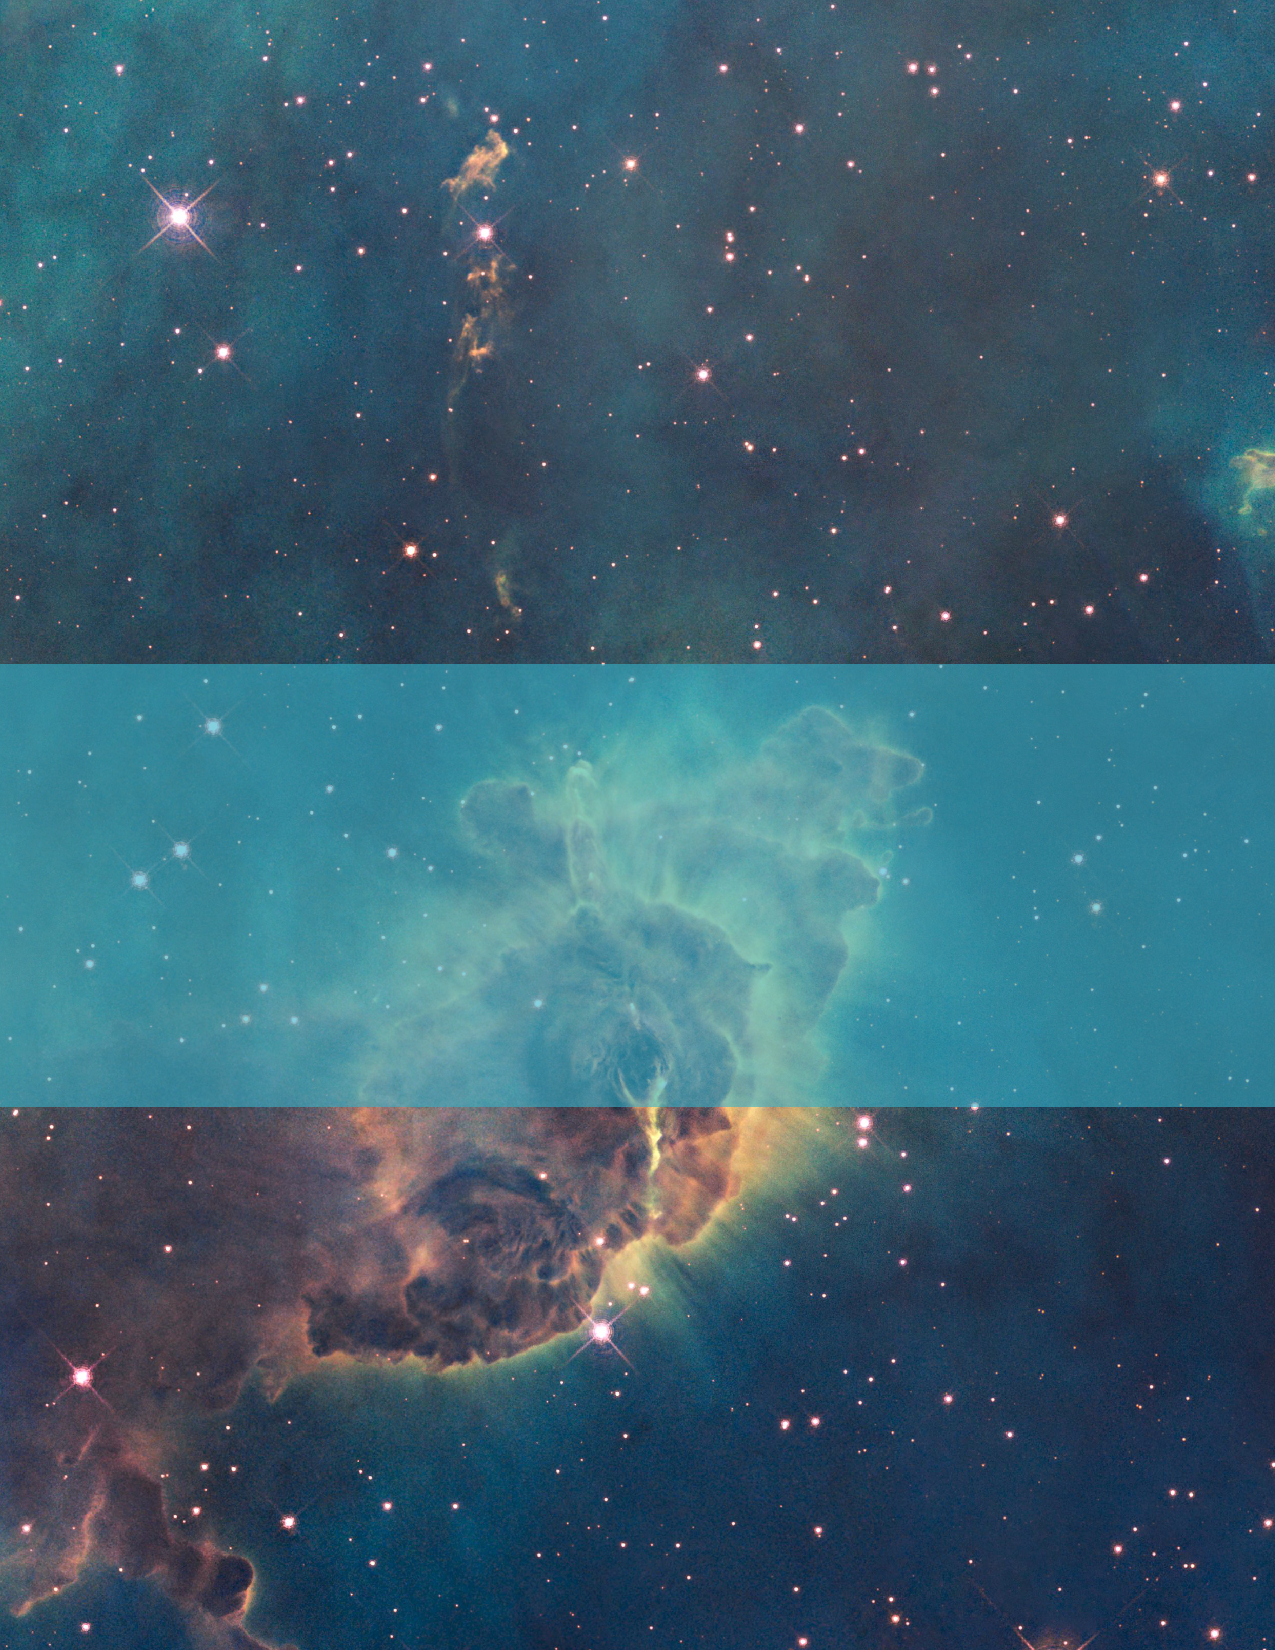
\includegraphics[scale=1.25]{esahubble}}} % Image background
\centering
\vspace*{5cm}
\par\normalfont\fontsize{35}{35}\sffamily\selectfont
\textbf{Programação em Processing}\\
{\LARGE Sebenta - Escola das Artes}\par % Book title
\vspace*{1cm}
{\Huge Jorge C. S. Cardoso}\par % Author name
\endgroup

%----------------------------------------------------------------------------------------
%	COPYRIGHT PAGE
%----------------------------------------------------------------------------------------

\newpage
~\vfill
\thispagestyle{empty}

%\noindent Copyright \copyright\ 2014 Andrea Hidalgo\\ % Copyright notice

\noindent \textsc{Summer Research Internship, University of Western Ontario}\\

\noindent \textsc{github.com/jorgecardoso/ProgramacaoProcessing}\\ % URL

\noindent This research was done under the supervision of Dr. Pauline Barmby with the financial support of the MITACS Globalink Research Internship Award within a total of 12 weeks, from June 16th to September 5th of 2014.\\ % License information

\noindent \textit{First release, August 2014} % Printing/edition date

%----------------------------------------------------------------------------------------
%	TABLE OF CONTENTS
%----------------------------------------------------------------------------------------

\chapterimage{head1.png} % Table of contents heading image

\pagestyle{empty} % No headers

\tableofcontents % Print the table of contents itself

%\cleardoublepage % Forces the first chapter to start on an odd page so it's on the right

\pagestyle{fancy} % Print headers again

%%----------------------------------------------------------------------------------------
%	CHAPTER 1
%----------------------------------------------------------------------------------------

\chapterimage{head2.png} % Chapter heading image

\chapter{Introduction}

\section{Motivation}\index{Motivation}
When I applied for the summer research internship, the title of the project was \emph{The many colours of nearby galaxies} an the description was
\begin{quote}
The different populations of stars in a galaxy carry the record of its past star formation history, and also affect its future. The project involves  analyzing Hubble Space Telescopes images of nearby galaxies of different types. By measuring the brightness and colours of millions of stars, we can understand the ages and compositions of the stars, and learn how the galaxy formed stars in the past. The radiation emitted by stars affects the gas in a galaxy, and thus how it will form stars in the future. We will use multi-colour images of galaxies to gain new insights into both their past and future.
\end{quote}

So, as an engineer without any astrophysics background I thougth I would be doing image processing applied to astronomy and I ended up doing so much more, but hey! You never know what you will end up doing.

Before comming to Canada, Pauline and I exchanged some emails where she shared me some interesting papers, webpages and an astronomy online course which later I did take, mainly the information was about a general introduction to astronomy and how astronomy images are, yes, astronomy images are completely different as any other \emph{normal} images, they are made of purely science data and every image has valuable knowledge you can learn from, and hey you will forget soon about pixels and start talking about sky coordinates.

So, in a few words I had no idea of what I was going to do (still), I realized I didn't have any idea, and the only thing I undestood was how CCD detectors work. I didn't know I had a research adventure awaiting for me.

\section{Objective}\index{Objective}
After I arrived and had my first meeting with Pauline, she explained me a general idea of what she wanted and shared me some more papers (about multi-wavelenght studies), I read the information and came up with the objective.

\begin{itemize}
\item Find out a method to transform data from a high dimensional dataset (FITS cube or any other data arrangement) to a low dimensional understandable information (graphs, clusters).
\end{itemize}

This means that from multiple images with different wavelengths of the same target apply an algorithm to find the hidden patterns that lie hidden between them.

\section{A bit of context}\index{Context}
Ok, here is where I explain from where this is going to start, at that time I just had a microcontrollers and engineering design course my mind was set completelly to find appplicable theories and create uselful things with them, which is the complete opposite of how astronomy works. First, there's no way to test an experiment with galaxies and most of the information is fuzzy and subjective (not all). The process of having an, let's say \emph{astronomy idea} is a result of applying all your physics knowledge and consider the \textbf{cosmological principle},
\begin{quote}
The (testable) assumption that the same physical laws that apply here and now also apply everywhere and at all times, and that there are no special locations or directions in the universe.
\end{quote}

That's how science is made, thinking and testing and thinking again, creating your own scientific method, comming up with hypothesis, learning what might work and what not, using your insticts. 

Well, before comming here I didn't think like that, it was just all about being super productive and thinking about doing robots and all kinds of devices with sensors. I had some experience programming in C/C++, no computer science backgound and I had never had an astronomy course.

This report was written in order to help someone to continue researching about data mining techniques applied in Astronomy, I explain how did I come up with the clustering techniques, my hypothesis, some tests and other ideas I have had, I hope this can help anyone and the research is continued. Anything you may need/questions do not hesitate to contact me, my e-mail address is: \emph{mrs.petzl@gmail.com}, also s part of my own documentation I created a GitHub page where you can download all the codes I programmed and find more information. The link to this page is: \url{https://github.com/LaurethTeX/Clustering}, from the \textsc{readme} file you can acces to all the pages, take your time to surf.
%------------------------------------------------

\subsection{References}\index{References}

Since I found so much good information about pretty much everything I wanted to know about, I will just create a remark and let you know where you can find more specific information about, just like below.

\begin{remark}
For more information about the cosmological principle, review Chapter 1: Why Learn Astronomy?, page 10, from \textbf{21st Century Astronomy}, \textit{Hester | Smith | Blumenthal | Kay | Voss}, Third Edition, 2010.
\end{remark}

%This statement requires citation \cite{book_key}; this one is more specific \cite[122]{article_key}.



\chapterimage{band1.png}
\chapter{Introdução - o que é programar?}

Este capítulo pretende dar apenas uma visão geral do que significa programar um computador. O leitor mais ávido por começar a experimentar pode avançar para o próximo capítulo.

\section{Programação}
``Programar'', no contexto deste manual, significa especificar um conjunto de instruções para serem executadas por uma máquina. No entanto, pode ser instrutivo fazermos a analogia máquina--pessoa para ilustrar alguns conceitos associados à programação de computadores, i.e., pensarmos em exemplos do nosso quotidiano e imaginarmo-nos a ``executar um programa''.

%Estas instruções, ou passos, não são mais do que ``comandos'' que a máquina ou pessoa deve executar para chegar ao objectivo final. 

\begin{lstlisting}[caption={Receita de pipocas. Adaptado de \url{http://lifestyle.sapo.pt/sabores/receitas/pipocas-doces-caseiras}.}, label=exe:receitaPipocas]
Cobre-se o fundo de um tacho com milho sem, no entanto, sobrepor. 
Rega-se o milho com um pouco de óleo e leva-se a lume brando, com o tacho tapado. 
Quando o milho começar a estalar agita-se o recipiente (sempre tapado).
Deixa-se cozinhar enquanto as pipocas estalam. 
Desliga-se, então, o lume mas só se retira a tampa quando o matraquear cessar completamente.
Agora, o adoçar: o tacho vai a lume brando, com o fundo coberto de açúcar. 
Deita-se as pipocas dentro do tacho e, quando o açúcar começar a ficar líquido, envolve-se com as pipocas utilizando para o efeito uma colher de pau. 
Movimenta-se as pipocas em sentido circular para se agarrarem ao açúcar. 
O tacho sai do lume quando o açúcar se torna amarelado.
Continua-se a mexer as pipocas até o açúcar desaparecer completamente.
\end{lstlisting}

%Se estivermos a definir um programa para ser seguido por um ser humano, as instruções que lhe damos são muito diferentes das
%instruções que dariamos a um computador. 
Por exemplo, o seguinte programa para abrir a porta quando alguém bate seria facilmente seguido por uma pessoa%
\footnote{Os programas mostrados nesta secção utilizam uma sintaxe livre, i.e.%
, não estão escritos numa linguagem de programação particular. Estão escritos em pseudo-código, ou seja, uma linguagem utiliza apenas para comunicar programas entre 
pessoas. Estes programas não podem ser executados num computador, servem apenas para efeitos de exemplificação dos conceitos básicos.}%
:
\begin{lstlisting}[caption=Programa ``Atender a porta'', label=exe:atenderPorta]
esperar que alguém bata à porta.
levantar da cadeira.
dirigir-se à porta.
abrir a porta.
perguntar em que pode ajudar.
\end{lstlisting}

Este primeiro exemplo serve para ilustrar algumas características da programação.
Primeiro, a ordem das instruções é extremamente importante; as linhas estão numeradas para dar relevância a esse facto. O programa não funcionaria se a execução trocasse a ordem de uma das instruções para, por exemplo:

\begin{lstlisting}[caption=Programa ``Atender a porta'' com instrução trocada, label=exe:atenderPortaOrdemTrocada]
levantar da cadeira.
dirigir-se à porta.
abrir a porta.
esperar que alguém bata à porta.
perguntar em que pode ajudar.
\end{lstlisting}

Segundo, as instruções são escritas na forma imperativa. Ao programar podemo-nos imaginar a dar ordens a quem executa o programa.

O Exemplo~\ref{exe:atenderPorta} ilustra ainda uma outra característica dos programas de computador: a entrada e saída de dados. Um programa não seria muito útil se não produzisse nada que pudesse ser utilizado pela pessoa que o executa. A saída de um programa pode tomar várias formas, e.g., números no ecrã, uma folha de papel na impressora, efeitos visuais, som, actuação física de motores de um robô, etc. Da mesma forma, a maioria dos programas permitem que o utilizador introduza, de alguma forma, dados que serão manipulados por esse programa. A forma mais típica de introdução de dados é através do rato e teclado, mas um programa pode obtê-los através de várias formas, como leitura de um ficheiro previamente escrito, leitura de sensores ligados ao computador, imagens de cameras web, áudio do microfone, etc. 



%O programa anterior seria facilmente executado por uma pessoa, mas não por um computador. O programa é demasiado ambíguo para ser executado por uma máquina. Por exemplo, o que aconteceria se a sala tivesse várias portas? Logicamente, uma pessoa iria atender a porta de onde veio o som... mas uma máquina não tem este tipo de compreensão. A instrução 
%\begin{verbatim}
%3 - dirigir-se à porta
%\end{verbatim}
%é demasiado vaga para uma máquina -- é necessário especificar qual a porta para onde devemos dirigirmo-nos. Os programas de computador necessitam, por isso, de um conjunto de instruções precisas que o computador (ou melhor, o processador do computador) saiba executar.



%\section{Algoritmos}
%Normalmente fazemos a distinção entre \emph{algoritmo} e \emph{programa}. Estes dois conceitos estão intimamente relacionados mas têm significados ligeiramente diferentes:
%\begin{description}
%\item[Algoritmos]
%Um algoritmo%
%\footnote{A palavra algoritmo tem origem no nome do matemático persa Al-Khwarizmi - 780-850.}
%é um ``conjunto de regras e operações que permitem resolver, num número finito de etapas, um problema''\cite{infopedia}.
%
%\item[Programa]
%Um programa de computador é um ``conjunto completo de instruções, em linguagem de código, que indica ao computador, passo a passo, como determinada tarefa deverá ser executada''\cite{infopedia}.
%\end{description}
%
%Dito de forma mais simples, um programa é uma implementação concreta de um algoritmo.
%
%É útil fazer esta distinção porque a definição de um algoritmo permite-nos comunicar a resolução de um problema sem nos preocuparmos com os detalhes sintácticos ou semânticos de uma determinada linguagem de programação.
%
%Normalmente os algoritmos são especificados em linguagem natural, i.e.%
%\footnote{\emph{i.e.} -- significa \emph{isto é} (do latim, \emph{id est}).}%
%, em Português, ou em pseudo-código -- uma linguagem intermédia entre a natural e uma linguagem de programação. 
%Os programas são escritos numa determinada linguagem de programação, e.g.%
%\footnote{\emph{e.g.} -- significa \emph{por exemplo} (do latim, \emph{exempli gratia}).}%
%, Processing, C, Java, ActionScript, PHP, etc.


\section{Como Funciona o Processador de um Computador}


%\section{História Resumida das Linguagens de Programação}


\section{Linguagens de Programação}
Existem várias linguagens que podemos utilizar para programar. Algumas apenas funcionam em determinados ambientes, por exemplo, o ActionScript é uma linguagem para programar Flash, ou seja apenas funciona no programa Macromedia Flash.
O PHP, por outro lado, serve apenas para programar páginas web, i.e., não podemos criar um programa com janelas e botões em PHP.
A linguagem C, por outro lado é uma linguagem mais tradicional -- serve para escrever programas que correm directamente no computador.

Apenas como curiosidade, aqui fica uma pequena lista das linguagens de programação mais comuns:
\begin{description}
\item[Processing]
Uma linguagem de programação baseada na linguagem Java. Criada para simplificar a programação em Java e para servir como ferramenta para artistas digitais e para o ensino da programação.

\item[Java] 
Uma linguagem de programação criada em 1995 como o objectivo de permitir a criação de programas que possam ser executados em várias plataformas sem modificação. A sua utilização tornou-se mais conhecida através das \emph{applets} -- pequenos programas que podem ser executados num browser. Os programas escritos em Java são compilados num código máquina virtual que é depois (aquando da execução do programa) transformado em código máquina real.

\item[C/C++] 
Uma das linguagens mais utilizadas e mais antigas no mundo. A sintaxe é muito parecida com a do Java (a sintaxe do Java foi inspirada no C). Um programa escrito em C tem de ser compilado para código máquina antes de poder ser executado.

\item[PHP] 
O PHP não é bem uma linguagem de programação, no sentido em que não permite a criação de programas de computador como os entendemos geralmente. O PHP não permite criar um programa (com janelas, menus, botões, etc) para ser executado num computador pessoal. Esta linguagem é destinada à criação de páginas Web e, por isso, os programas escritos em PHP não são compilados em código máquina. Um programa PHP é executado pelo servidor Web; por esta razão diz-se que o PHP é uma linguagem de \emph{scripting}%
\footnote{Uma linguagem de scripting é uma linguagem em que os programas precisam de um outro programa para executar. O PHP precisa de um servidor Web para executar o seu código, por exemplo. O ActionScript precisa do Flash Player para correr...}

%\item[ActionScript]
%Uma linguagem de scripting utilizada para programar em Flash.

%\item[VisualBasic]
%Uma linguagem de programação para o sistema Windows, introduzida pela Microsoft. 

\end{description}

\subsection{Compilar e Executar}
Nos primórdios da computação, a programação de um computador era feita usando instruções entendidas directamente pelo computador. Estas instruções são designadas por código máquina. Computadores diferentes (com processadores diferentes) possuem conjuntos de instruções diferentes, pelo que um programa escrito em código máquina apenas executa num determinado tipo de computador. 
A programação em código máquina era muito trabalhosa e propícia a erros (as instruções são compostas por '0's e '1's), pelo que era necessário pessoal altamentente especializado para efectuar a tarefa de programação de um computador.

À medida que a área avançou apareceram novas formas de programar: em vez de escrevermos um programa em código máquina, por que não escrever numa linguagem mais próxima da linguagem natural e fazer um programa que converta entre a linguagem natural (a usada pelo programador) e a linguagem máquina? Foi então que surgiram as primeiras linguagem de programação de alto nível%
\footnote{Uma linguagem de alto nível é uma linguagem com uma sintaxe mais próxima da linguagem natural do que a linguagem em código máquina.}%
.

Associado às linguagens de alto nível está um tipo de programa especial: o compilador. O compilador não é mais do que um programa que converte o programa escrito pelo programador em linguagem de alto nível para código máquina de forma a poder ser executado pelo computador. O programa escrito pelo programador é designado por \emph{código fonte}.


\section{Lógica e Sintaxe}
O código fonte de um programa pode ser visto de duas perspectivas: da lógica do programa; e da sintaxe.

Uma determinada linguagem de programação é definida principalmente pela sua sintaxe, ou seja pelas regras que definem o que é um programa bem escrito. Da mesma forma que a sintaxe da língua Portuguesa define as regras de construção de frases, também a sintaxe da linguagem de programação define as regras de construção de um programa escrito nessa linguagem. Por exemplo, a frase ``O João foi às compras.'', está de acordo com as regras, mas ``O João às foi compras.'', não está. Apesar de o significado de ambas as frases ser óbvio e idêntico: o João foi às compras, a segunda quebra as regras da construção de frases em Português.

A lógica de um programa equivale ao seu significado. No exemplo anterior a lógica (significado) da frase era óbvia, mas estava mal construida. Também um programa pode estar logicamente correcto, mas sintacticamente incorrecto. Um programa sintacticamente incorrecto não pode ser compilado (os compiladores não são ``suficientemente inteligentes'' para perceberem o significado do programa de modo a corrigirem a sintaxe). Os erros sintácticos são facilmente detectados pelo compilador.
De forma inversa, um programa pode estar sintacticamente correcto, mas logicamente não. Nestes casos, o programa é compilado e executado, mas o resultado não é o que o programador estava à espera. Estes erros são mais difíceis de detectar!




\section{Nível de Detalhe}
Quando escrevemos um programa em Português a que nível de detalhe devemos ir na especificação das instruções?
Por exemplo, se quisermos escrever um programa para uma pessoa mudar um pneu de um carro podemos ter algo como o seguinte:
\begin{verbatim}
1 - sair do carro.
2 - abrir a mala do carro.
3 - tirar pneu sobresselente.
4 - tirar macaco.
5 - tirar chave.
6 - desapertar ligeiramente as porcas do pneu.
7 - colocar o macaco debaixo do carro.
8 - dar \'a manivela até o pneu ficar suficientemente levantado.
9 - desapertar as porcas na totalidade.
10 - retirar o pneu furado.
11 - colocar o pneu novo.
12 - apertar as porcas.
13 - baixar o carro.
14 - retirar o macaco.
15 - apertar bem as porcas.
16 - guardar chave.
17 - guardar macaco.
18 - guardar pneu furado.
\end{verbatim}

Mas, estamos a assumir que a pessoa sabe fazer uma série de coisas, como sair do carro, abrir a mala, etc.
Cada um dos passos do nosso programa anterior pode ele mesmo ser um programa em si. Por exemplo sair do carro:
\begin{verbatim}
1 - desligar o carro.
2 - apertar o travão de mão.
3 - retirar o cinto de segurança.
4 - retirar a chave da ignição.
5 - abrir a porta.
6 - sair.
7 - fechar a porta.
\end{verbatim}

Então, a que nível de detalhe deveremo ir quando estamos a escrever um programa? No caso de um programa para ser executado por uma pessoa, devemos descer ao nível de detalhe suficiente para a pessoa conseguir executar cada passo. Obviamente, isto depende da tarefa e da pessoa.

No caso de um programa de computador, o problema não se coloca a este nível. Ao utilizarmos uma determinada linguagem de programação, estamos automaticamente limitados às instruções mais básicas fornecidas por essa linguagem. Por exemplo, no caso do desenho num ecrã, algumas linguagens apenas possuem instruções para desenhar um pixel numa determinada posição do ecrã. Neste caso, se quisermos fazer uma programa para desenhar uma linha vertical teriamos de fazer algo do género:
\begin{verbatim}
1 - desenhar pixel na primeira posicao da linha.
2 - avancar um pixel na vertical.
3 - desenhar um pixel na nova posicao.
4 - repetir o passo 2 até chegar ao final da linha.
\end{verbatim}

Outras linguagens têm instruções para desenhar linhas, pelo que o programa anterior se resumiria a uma única instrução:
\begin{verbatim}
1 - desenhar linha vertical.
\end{verbatim}

Ou seja, quando programamos um computador temos de utilizar as instruções fornecidas pela linguagem que estamos a utilizar. Daí que algumas linguagens sejam mais aplicadas nalguns tipos de programas -- possuem instruções que facilitam a escrita de determinados programas.

No entanto, o problema do nível de detalhe coloca-se sob outra perpectiva quando programamos um computador. Todas as linguagens permitem-nos definir as nossas próprias instruções compostas por sequências maiores de instruções básicas. Por exemplo, no caso da linguagem que apenas permite desenhar um pixel numa posição do ecrã, poderiamos compor uma nova instrução: \texttt{desenharLinhaVertical}, à custa dos passos do nosso programa exemplo. Assim, sempre que quisessemos desenhar uma linha vertical no ecrã bastava usar a nova instrução:
\begin{verbatim}
1 - desenharLinhaVertical.
\end{verbatim}

Quando escrevemos um programa devemos pensar em agrupar conjuntos de instruções de forma a termos ao nosso dispor instruções que efectuam vários passos de cada vez. 
A questão agora é saber que instruções agrupar. Novamente, não há uma resposta única. Depende do programa. É uma questão de experiência (e, às vezes, de estilo do programador).

\section{Conceitos Básicos de Um Programa}
Quando criamos programas, ou, de forma mais genérica, quando pensamos em algoritmos, existem alguns conceitos fundamentais que são comuns a todos eles: \emph{memória}, \emph{selecção} e \emph{iteracção}.

\begin{description}
\item[memória]\footnote{O conceito de memória será aprofundado no Capítulo~\ref{cap:memoria}.}
A memória é o que permite ao nosso programa guardar dados temporários ou intermédios para serem utilizados mais tarde.
Por exemplo, se pretendessemos criar um programa para calcular os pontos da equipa do FCP no campeonato fariamos algo do género:
\begin{verbatim}
1 - ler jogosGanhos.
2 - ler jogosEmpatados.
4 - pontos = jogosGanhos * 3 + jogosEmpatados.
5 - escrever pontos.
\end{verbatim}
No programa anterior a instrução \texttt{ler}, coloca numa \emph{variável} um valor fornecido pelo utilizador. Uma variável
é a memória do nosso programa. É como uma gaveta com nome, na qual podemos guardar valores para mais tarde utilizar.
O programa anterior precisa de guardar os valores do número de jogos ganhos e empatados para poder efectuar a operação matemática que devolve o número de pontos no campeonato. O resultado desse cálculo, é, ele mesmo, colocado também numa ``gaveta'' para posterior utilização. Uma vez colocados na ``gaveta'' (variável), os dados podem ser consultados em qualquer altura (ponto de execução) do nosso programa. 

\item[selecção] \footnote{O conceito de selecção será aprofundado no Capítulo~\ref{cap:seleccao}.}
O conceito de \emph{selecção} está associado ao caminho executado pelo nosso programa. Um programa pode ser visto como uma árvore: a execução começa por um ponto comum -- o tronco, e, à medida que o programa executa, pode percorrer um ramo ou outro, dependendo das circunstâncias no momento da execução.
Por exemplo, no programa seguinte:
\begin{verbatim}
1 - ler jogosGanhosFCP.
2 - ler jogosEmpatadosFCP.
3 - ler jogosGanhosSLB.
4 - ler jogosEmpatadosSLB.
5 - pontosFCP = jogosGanhosFCP * 3 + jogosEmpatadosFCP.
6 - pontosSLB = jogosGanhosSLB * 3 + jogosEmpatadosSLB.
7 - se pontosFCP > pontosSLB então
    8 - escrever "O FCP está à frente do SLB".
9 - senão
    10 - escrever "O SLB está à frente do FCP".     
\end{verbatim}

existe um ``tronco'' comum a todas as execuções do programa -- as linhas de 1 a 7.
No entanto, consoante a pontuação de uma e outra equipa, o programa pode percorrer o ramo 8 -- se o FCP tiver mais pontos que o SLB, ou o ramo 10 -- se o SLB tiver mais pontos que o FCP.
A linha 7 -- \texttt{se pontosFCP > pontosSLB}%
\footnote{O símbolo ``>'' significa ``maior do que''.}
\emph{selecciona} o ramo%
\footnote{As linhas 8 e 10 estão \emph{indentadas}, isto é, escritas mais à direita, para facilitar a leitura do programa. Desta forma é óbvio que o ramo 8 corresponde à condição ser verdadeira e o 10 à condição falsa. Caso contrário, não seria facilmente perceptível que o programa contém ramos.}
a executar no programa.

\item[iteracção]\footnote{O conceito de iteracção será aprofundado no Capítulo~\ref{cap:iteraccao}.}
A maior parte dos programas que escrevemos contêm partes que são repetidas várias vezes. Por exemplo, se quisermos calcular as pontuações de todas as equipas do campeonato, poderiamos construir um programa do género:
{\small
\begin{verbatim}
1 - ler jogosGanhosEquipa1.
2 - ler jogosEmpatadosEquipa1.
3 - pontosEquipa1 = jogosGanhosEquipa1 * 3 + jogosEmpatadosEquipa1.
4 - escrever pontosEquipa1.
5 - ler jogosGanhosEquipa2.
6 - ler jogosEmpatadosEquipa2.
7 - pontosEquipa2 = jogosGanhosEquipa2 * 3 + jogosEmpatadosEquipa2.
8 - escrever pontosEquipa2.
9 - ler jogosGanhosEquipa3.
10 - ler jogosEmpatadosEquipa3.
11 - pontosEquipa3 = jogosGanhosEquipa3 * 3 + jogosEmpatadosEquipa3.
12 - escrever pontosEquipa3.
...
68 - ler jogosGanhosEquipa18.
70 - ler jogosEmpatadosEquipa18.
71 - pontosEquipa18 = jogosGanhosEquipa18 * 3 + jogosEmpatadosEquipa18.
72 - escrever pontosEquipa18.
\end{verbatim}}
Neste programa, para calcular a pontuação de 18 equipas, precisamos de 72 linhas de código! No entanto, se olharmos bem, as linhas são muito parecidas -- as primeiras 4 linhas repetem-se ao longo do programa. Existe uma estrutura que nos permite economizar linhas de código: o \emph{ciclo}. Vejamos o seguinte programa:
{\small
\begin{verbatim}
1 - i = 1.
2 - enquanto i <= 18 fazer
    3 - ler jogosGanhosEquipa.
    4 - ler jogosEmpatadosEquipa.
    5 - pontosEquipa = jogosGanhosEquipa * 3 + jogosEmpatadosEquipa.
    6 - escrever pontosEquipa.
    7 - i = i + 1.
\end{verbatim}}
Neste caso, colocamos as 4 linhas repetidas do programa anterior dentro daquilo a que chamamos \emph{ciclo} -- uma estrutura que repete a execução das linhas de código (iterativa)%
\footnote{Não confundir \emph{iteractiva} -- que se repete; com \emph{interactivo} -- que permite a troca de informação entre sistema e utilizador.}%
. 
Basicamente, o programa utiliza uma variável para contar as equipas que já calculámos: a variável \texttt{i}. Enquanto 
codificação.

\end{description}



\section{Exercícios}

\subsection{Resolvidos}

\begin{enumerate}
	\item \label{exe:1_1} Escreva um programa em linguagem natural para ligar os computadores de uma sala de aulas. Escreva o programa para ser seguido por uma pessoa. O programa deve ter pelo menos uma tomada de decisão.
	
	\item \label{exe:1_2} Baseando-se no programa que escreveu no ponto anterior, substitua cada instrução desse programa por um conjunto de instruções mais detalhadas.
	
	\item \label{exe:1_3} 
\end{enumerate}

\subsection{Para Resolver}
\begin{enumerate}
\item 
Pensar num programa que possa ser facilmente implementado por um colega seu na sala de aula. Escrever esse programa.  O programa deve ter mais de 10 instruções, deve ter pelo menos uma estrutura de selecção ou iteracção e deve poder ser executado em menos de 5 minutos.

\item Escreva o programa anterior com um nível de detalhe maior.

\item (Tentar) Agrupar as novas instruções em conjuntos de instruções maiores e diferentes do original.
\end{enumerate}

\subsection{Resolução dos Exercícios Resolvidos}

{\footnotesize
\subsubsection*{Exercício \ref{exe:1_1}}
\begin{verbatim}
Programa Ligar os Computadores da Sala

1 - Dirigir-se ao primeiro computador.
2 - Carregar no botão de ``power'' do computador.
3 - Carregar no botão de ``power'' do monitor.
4 - Se computador não ligou
    5 - Verificar cabos de alimentação
    6 - Repetir o passo 2.
7 - Verificar se há mais computadores     
8 - Se houver mais computadores então
    9 - Dirigir-se ao computador seguinte.
    10 - Repetir o passo 2.
11 - Senão
    12 - Termina.    
\end{verbatim}}
\paragraph{Notas}
Este programa funciona apenas se determinadas condições se verificarem. Uma vez que 
não colocámos instruções para verificar se o computador já estava ligado, caso
isso aconteça o computador será desligado. Para o programa funcionar como
pretendido é necessário que todos estejam desligados.


\subsubsection*{Exercício \ref{exe:1_2}}
{\footnotesize
\begin{verbatim}
Programa Ligar os Computadores da Sala (mais detalhe)

1 - Dirigir-se ao primeiro computador.
2 - Verificar se o computador está desligado.
3 - Se o computador estiver desligado então
    4 - Identificar botão de ``power'' do computador.
    5 - Levantar a mão e esticar o dedo indicador.
    6 - Pressionar o botão de ``power'' do computador.
7 - Verificar se o monitor está desligado.
8 - Se o monitor estiver desligado então
    9 - Identificar botão de ``power'' do monitor.
    10 - Levantar a mão e esticar o dedo indicador.
    11 - Pressionar o botão de ``power'' do monitor.
12 - Se computador não ligou
    13 - Verificar cabos de alimentação do computador.
    14 - Verificar os cabos de alimentação do monitor.
    15 - Repetir o passo 3.
16 - Verificar se há mais computadores     
17 - Se houver mais computadores então
    18 - Dirigir-se ao computador seguinte.
    19 - Repetir o passo 2.
20 - Senão
    21 - Termina.    
\end{verbatim}}

\subsubsection*{Exercício \ref{exe:1_3}}
{\footnotesize
\begin{verbatim}
Programa Ligar os Computadores da Sala (mais detalhe)

Instrução Ligar o Computador:
1 - Verificar se o computador está desligado.
2 - Se o computador estiver desligado então
    3 - Identificar botão de ``power'' do computador.
    4 - Levantar a mão e esticar o dedo indicador.
    5 - Pressionar o botão de ``power'' do computador.
6 - Fim Instrução    

Instrução Ligar o Monitor:
1 - Verificar se o monitor está desligado.
2 - Se o monitor estiver desligado então
    3 - Identificar botão de ``power'' do monitor.
    4 - Levantar a mão e esticar o dedo indicador.
    5 - Pressionar o botão de ``power'' do monitor.
6 - Fim Instrução

1 - Dirigir-se ao primeiro computador.
2 - [Ligar o Computador]
3 - [Ligar o Monitor]
12 - Se computador não ligou
    13 - Verificar cabos de alimentação do computador.
    14 - Verificar os cabos de alimentação do monitor.
    15 - Repetir o passo 2.
16 - Verificar se há mais computadores     
17 - Se houver mais computadores então
    18 - Dirigir-se ao computador seguinte.
    19 - Repetir o passo 2.
20 - Senão
    21 - Termina.
\end{verbatim}}

\chapterimage{band1.png}
\chapter{Processing}
O Processing é uma linguagem/ferramenta de programação baseada na linguagem de programação Java.
A ideia por detrás da génese do Processing era a criação de uma linguagem para programação de efeitos visuais que
fosse mais fácil de utilizar do que as existentes. Basicamente, o Processing simplifica a programação ao esconder alguns conceitos e alguma da complexidade da programação em Java, ao mesmo tempo de fornece um ambiente de ensino da programação orientado para artistas digitais.

Este capítulo procura enquadrar a utilização do Processing mostrando alguns exemplos de projectos, descreve o ambiente de desenvolvimento da ferramenta e aborda alguns conceitos básicos associados.

\section{O Que É?, Para Que Serve?}
A linguagem Processing tem sido utilizada predominantemente para aplicações artistícas. O Processing pode ser utilizado para instalações, \emph{web art}, \emph{video art}, etc. De seguida apresentam-se alguns projectos em que o Processing foi utilizado.

\begin{description}
\item[Nulltidão] Projecto desenvolvido por João Cordeiro no âmbito da cadeira de Programação Multimédia, em 2006. 
Este projecto consiste numa instalação vídeo que joga com os conceitos de multidão e individualidade. 
A instalação consiste num \emph{video-wall} que exibe um vídeo obtido em tempo-real a partir de uma \emph{web cam}. O vídeo
é manipulado de forma a mostrar apenas algumas regiões da imagem da \emph{web cam} sobrepostas a uma imagem inicial. A imagem inicial é uma \emph{frame} da \emph{web cam} tirada durante a montagem da instalação, de forma a não conter pessoas na imagem. O número de regiões do vídeo depende do número de pessoas a observar a instalação
A instalação usa a informação sobre a quantidade de dispositivos Bluetooth (telemóveis) perto da instalação como estimativa do número de pessoas a observar a instalação. 
\begin{center}
	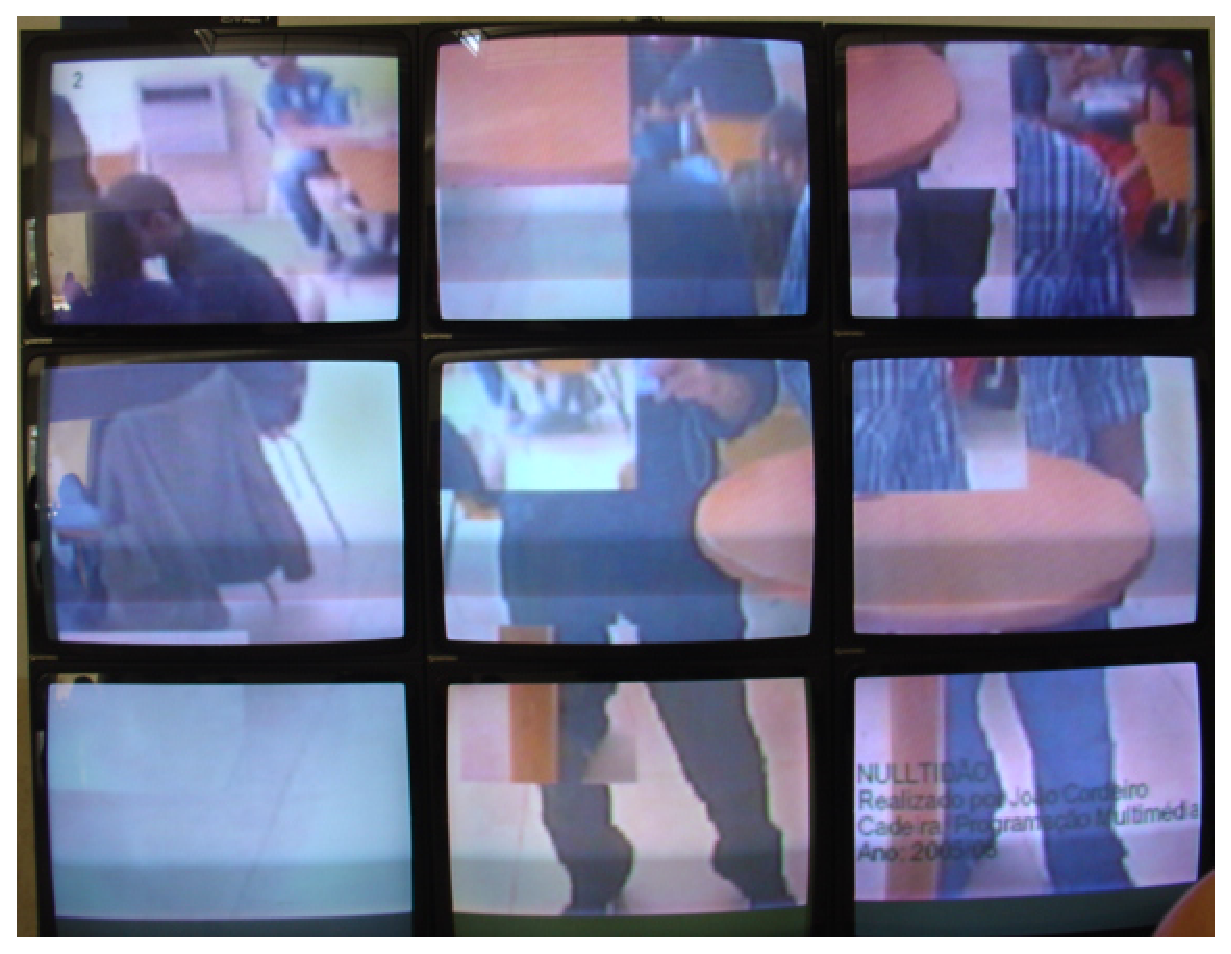
\includegraphics[width=8cm]{images//nulltidao}
\end{center}

\item[Shadow Monsters] \emph{Shadow Monsters} (\url{http://www.worthersoriginal.com/viki/#page=shadowmonsters}) é uma instalação interactiva que permite aos utilizadores projectarem sombras com as mãos. As sombras são modificadas de forma a se transformarem em monstros. 
\begin{center}
	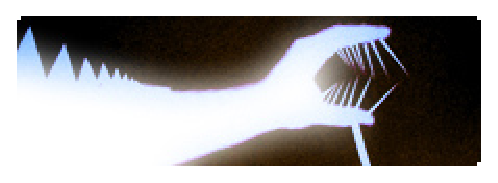
\includegraphics{images/shadowmonsters.eps}
\end{center}

\item[Nike 'One'] O anúncio realizado pela Motion Theory para a Nike (\url{http://www.motiontheory.com/work/nike_one}) foi programado parcialmente em Processing. O programa utilizado pode ser visto separadamente em \url{http://dev.motiontheory.com/nikegolf/}.
\begin{center}
	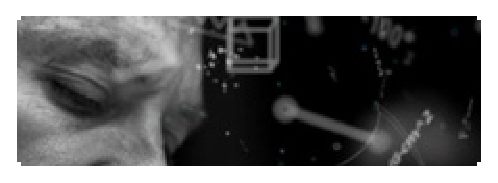
\includegraphics{images/nikeone.eps}
\end{center}

\item[The Dumpster]
O \emph{Dumpster} (\url{http://artport.whitney.org/commissions/thedumpster/}) é uma ``visualização \emph{online} que tenta 
mostrar uma fatia da vida romântica dos adolescentes Americanos. A aplicação usa \emph{posts} reais extraídos de milhões
de blogs e gera uma visualização que permite navegar entre as secções em que uma pessoa ``acabou'' com outra.''.
O projecto foi desenvolvido por Golan Levin, entre outros.
\begin{center}
	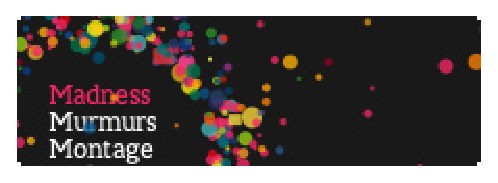
\includegraphics{images/wefeelfine.eps}
\end{center}

\end{description}

\section{Ambiente de Desenvolvimento}
O ambiente de desenvolvimento (\emph{Integrated Development Environment} -- IDE) do Processing é um pequeno editor que permite escrever e executar os programas. 
A Figura~\ref{fig:ide} mostra a janela do IDE. 
\begin{figure}[!hbp]
	\centering
		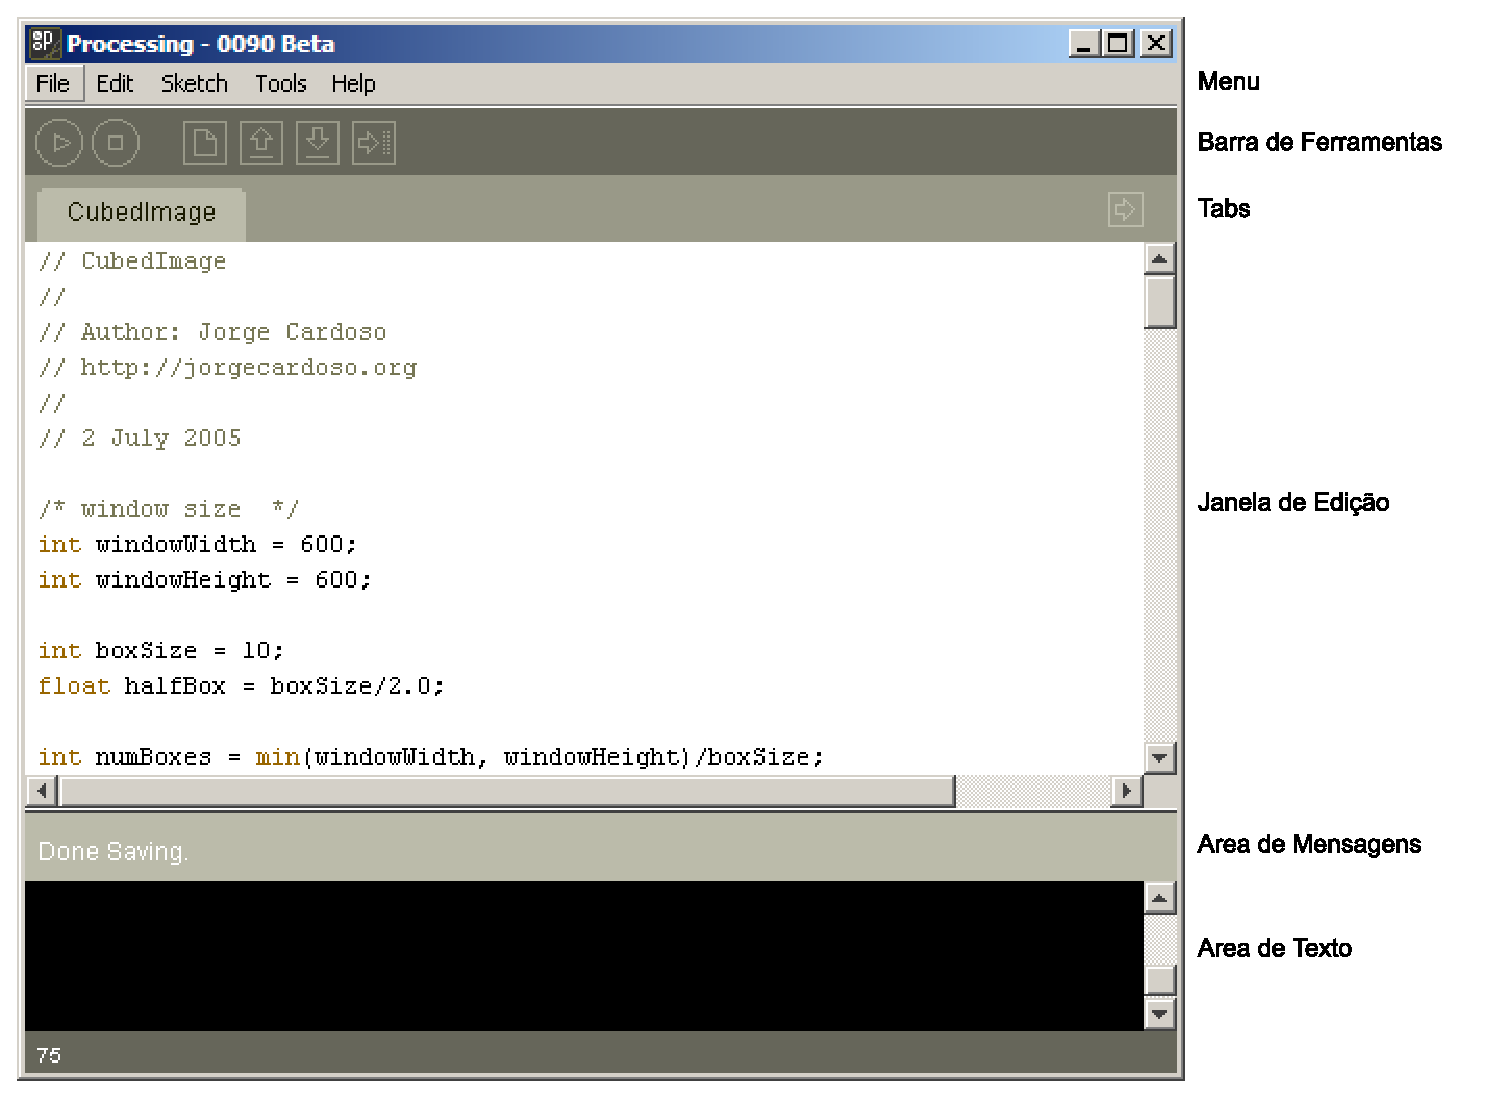
\includegraphics[width=.9\textwidth]{images/ide.eps}
	\caption{IDE do Processing}
	\label{fig:ide}
\end{figure}

A janela do editor está organizada, de cima para baixo, nos seguintes componentes:
\begin{description}
\item[Menu] ... descritos mais à frente.
\item[Barra de Ferramentas] Fornece um acesso rápido às funções Executar, Parar, Criar Novo Sketch, Abrir Sketch, Gravar Sketch e Exportar.
\item[\emph{Tabs}] Cada \emph{Tab} representa um \emph{sketch} aberto.
\item[Janela de Edição] A janela onde escrevemos o código do programa. A janela de edição possui \emph{sintax highlighting}.
\item[Área de Mensagens] Nesta área aparecem algumas mensagens de \emph{status} e os erros de compilação do programa.
\item[Área de Texto] Nesta área é mostrada a saída normal do programa bem como os possíveis erros que ocorram durante a execução.
\end{description}

\subsection{Menus}
Os menus do IDE são os seguintes:
\paragraph{File}
\begin{itemize} 
\item[New] Cria um novo \emph{sketch}.
\item[Sketchbook] Permite abrir um \emph{sketch} localizado no computador, ou um exemplo.
\item[Save] Grava o \emph{sketch} corrente.
\item[Save as...] Grava o \emph{sketch} corrente com um nome diferente.
\item[Export] Exporta o programa como uma \emph{applet} Java e correpondente ficheiro HTML.
\item[Export Application] Exporta o programa como uma aplicação Java para os sistemas Windows, Mac OS X e Linux. 
\item[Page Setup] (Não implementado ainda).
\item[Print] (Não implementado ainda).
\item[Preferences] Abre a janela de configuração do Processing.
\item[Quit] Termina o IDE e fecha todas as janelas.
\end{itemize}

\paragraph{Edit}
\begin{itemize}
\item[Undo] Desfaz o último commando aplicado.
\item[Redo] Desfaz o Undo.
\item[Cut] Remove e copia para o \emph{clipboard} o texto seleccionado.
\item[Copy] Copia para o \emph{clipboard} o texto seleccionado.
\item[Paste] Insere o conteúdo do \emph{clipboard} na posição do cursor.
\item[Select All] Selecciona todo o texto da janela de edição.
\item[Find] Procura uma ocorrência de uma palavra no texto e dá a opção de o substituir por outra palavra.
\item[Find Next] Procura a próxima ocorrência de uma palavra no texto.
\end{itemize}

\paragraph{Sketch}
\begin{itemize}
\item[Run] Executa o código. Este comando faz automaticamente a compilação do programa, abre a janela do programa e executa-o.
\item[Present] Executa o programa em \emph{fullscreen}.
\item[Stop] Se o programa estiver a executar, este comando termina-o.
\item[Add File] Permite adicionar um ficheiro de imagem ou outro tipo de dados à pasta de dados do projecto.
\item[Import Library] Adiciona as instruções de \emph{import} das bibliotecas ao programa corrente.
\item[Show Sketch Folder] Abre a pasta do projecto.
\end{itemize}

\paragraph{Tools}
\begin{itemize}
\item[Auto Format] Tenta formatar o código de forma a torná-lo mais legível.
\item[Create Font] Converte fontes no formato de fontes do Processing.
\item[Archive Sketch] Cria um ficheiro zip com o conteúdo do projecto.
\end{itemize}

\paragraph{Help}
\begin{itemize}
\item[Environment] Abre a página que descreve o ambiente de desenvolvimento do Processing.
\item[Reference] Abre  a página que contém a referência das funções do Processing.
\item[Find in Reference] Procura na referência, a palavra seleccionada no editor de texto.
\item[Visit Processing.org] Abre a página do Processing.org.
\item[About Processing] Painel de informação sobre o software.
\end{itemize}

\section{Obter o Processing}
O Processing pode ser descarregado a partir do site \url{processing.org}. Na secção \emph{download} existe a opção de descarregar 4 versões: duas para Windows (com ou sem Java -- devem descarregar a versão com Java), uma para Mac OS X e uma para Linux.



\section{Coordenadas}
O Processing utiliza um sistema de coordenadas cartesiano com a origem das coordenadas localizada no canto superior esquerdo do ecrã. O eixo dos XX é positivo para a direita e o eixo dos YY é positivo para baixo. No caso de estarmos a trabalhar em 3D, o eixo dos ZZ é positivo na direcção do utilizador.

A Figura~\ref{fig:coordinates} exemplifica o sistema de coordenadas.
\begin{figure}[htbp]
	\centering
		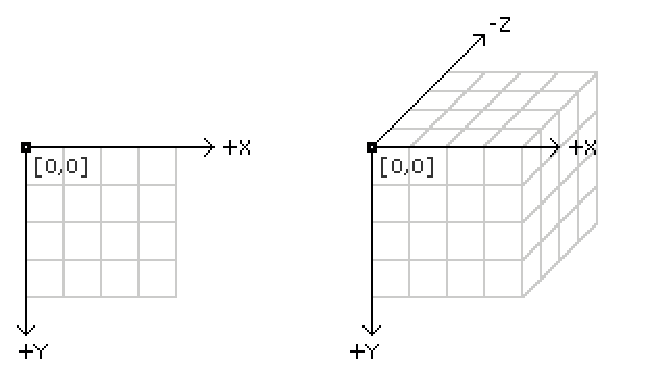
\includegraphics[width=10cm]{images/coordinates.eps}
	\caption{Sistema de coordenadas em Processing}
	\label{fig:coordinates}
\end{figure} 

\section{Compilar, Executar e Publicar}
Os programas em Processing precisam de ser compilados antes de serem executados. No entanto, no ambiente Processing, estes dois passos estão intimamente ligados: quando pressionamos no botão de executar, o nosso programa é automaticamente compilado e só depois executado.

A maior parte dos programas Processing são apresentados via Web, ou seja, são colocados numa página com uma applet. Para publicarmos o nosso programa, basta-nos aceder ao menu [File->Export]. Automaticamente, o Processing cria uma pasta nova dentro da pasta do nosso projecto com o nome \texttt{applet}. Nesta pasta encontramos cinco ficheiros:
\begin{description}
\item[index.html] A página html principal. Esta página contém o código que inclui a applet. 

\item[loading.gif] Uma imagem utilizada na applet enquanto o nosso programa está a ser carregado.

\item[NomeProjecto.jar] O nosso programa compilado e empacotado num ficheiro jar%
\footnote{Um ficheiro jar é basicamente um ficheiro comprimido (zip) com os ficheiros que compõem o nosso programa.}%
.

\item[NomeProjecto.java] O nosso programa Processing convertido em Java.

\item[NomeProjecto.pde] O nosso código fonte.
\end{description}

Se quisermos colocar o nosso programa online basta-nos copiar esta pasta para um servidor Web.

Uma outra forma de distribuir o nosso programa é através de uma aplicação que execute directamente no nosso computador (ao invés de executar através de um browser Web). Também podemos converter o nosso programa numa aplicação com o ambiente Processing. Para tal temos de aceder ao menu [File->Export Application]. Automaticamente, o Processing cria três pastas: \texttt{application.linux}, \texttt{application.macosx} e \texttt{application.windows}. Estas pastas contém as três versões da nossa aplicação, uma para cada sistema operativo.

\section{Alguns Exemplos}
\lstset{basicstyle=\scriptsize\ttfamily}

A partir desta secção o código utiliza a sintaxe do Processing.

Os exemplos seguintes foram retirados do site do Processing. 
Estes exemplos vêm com o Processing quando se descarrega e podem também ser vistos online na secção de exemplos da página do Processing.

\paragraph{Statements and Comments (Instruções e Comentários)}
\begin{center}
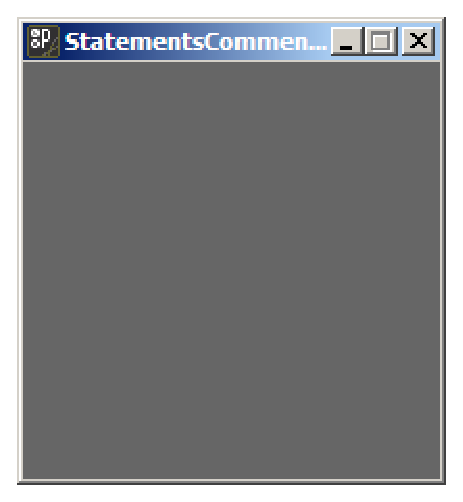
\includegraphics[width=4cm]{images/exemploStatementsComments.eps}
\end{center}
\begin{lstlisting}
// Statements and Comments
// by REAS <http://reas.com>

// Statements are the elements that make up programs.
// The ";" (semi-colon) symbol is used to end statements. 
// It is called the "statement terminator."
// Comments are used for making notes to help people better understand programs. 
// A comment begins with two forward slashes ("//").

// Created 1 September 2002

// The size function is a statement that tells the computer 
// how large to make the window.
// Each function statement has zero or more parameters. 
// Parameters are data passed into the function
// and used as values for specifying what the computer will do.
size(200, 200);

// The background function is a statement that tells the computer
// which color to make the background of the window 
background(102);
\end{lstlisting}

\paragraph{Width and Height (Largura e Altura)}
\begin{center}
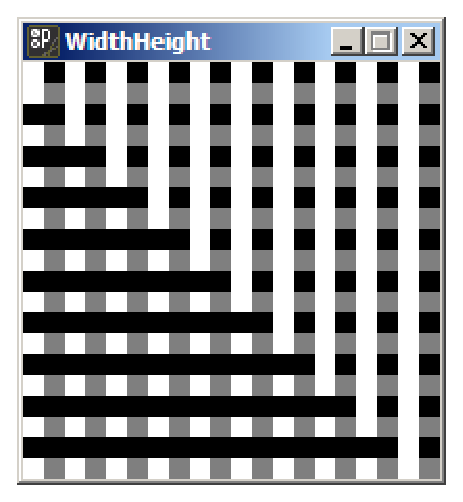
\includegraphics[width=4cm]{images/exemploWidthHeight.eps}
\end{center}
\begin{lstlisting}
// Width and Height
// by REAS <http://reas.com>

// The 'width' and 'height' variables contain the width and height 
// of the display window as defined in the size() function.

// Created 27 October 2002

size(200, 200);
background(127);
noStroke();
for(int i=0; i<height; i+=20) {
  fill(0);
  rect(0, i, width, 10);
  fill(255);
  rect(i, 0, 10, height);
}
\end{lstlisting}



\section[Modos de Programação]{Modos de Programação\protect\footnote{Traduzido e adaptado de \cite{Processing.orgProcessingEnvironmentVisitadoJaneiro2007}.}}
O Processing permite-nos programar em três níveis diferentes de complexidade: Modo Básico,
Modo Contínuo e Modo Java.
Deve-se começar pelo modo Básico para aprender a trabalhar com coordenadas, variáveis e ciclos antes
de passar para o modo Contínuo e modo Java.

\subsection{Modo Básico}
Neste modo apenas podemos programar imagens estáticas. Este modo é utilizado principalmente para aprender os fundamentos da programação. 
O exemplo seguinte desenha um rectângulo amarelo no ecrã%
\footnote{Todas as instruções neste exemplo são chamadas a métodos do Processing. Um método, ou função, é uma instrução básica do Processing, ou um agrupamento
de instruções básicas que se comporta como uma instrução básica. Os valores entre parentesis são os argumentos do método, i.e., valores que alteram a forma como o método se comporta. Os métodos são explicados no Capítulo~\ref{cap:metodos}.}
:
\begin{lstlisting}
size(200, 200);         // definir o tamanho da janela
background(255);        // colocar o fundo a branco
noStroke();             // indicar que as formas não têm border
fill(255, 204, 0);      // definir a cor de preenchimento - amarelo
rect(30, 20, 50, 50);   // desenhar um rectângulo (50x50) 
                        // na posição (30, 20)
\end{lstlisting}
Neste modo as instruções são interpretadas uma a uma e o programa termina quando a última for encontrada.

\subsection{Modo Contínuo}
O modo Contínuo fornece uma estrutura de programação em que é possível desenhar continuamente para o ecrã. Desta forma podemos construir animações. Neste modo é também possível obter \emph{input} do utilizador através do teclado e do rato.

Na sua forma mais básica, um programa neste modo é constituído por dois métodos: \texttt{setup()} e \texttt{draw()}. O método \texttt{setup()} serve para inicializar o programa -- este método executa apenas uma vez. O método \texttt{draw()} permite-nos desenhar para o ecrã -- este método é invocado repetidamente pelo sistema, permitindo-nos construir animações.


O exemplo seguinte desenha três círculos azuis semi-transparentes. Neste caso o método \texttt{draw()} apenas é executado uma vez, porque usamos o método \texttt{noLoop()} dentro do \texttt{setup()} para indicar que não queremos animação.
\begin{lstlisting}
void setup()
{
  size(200, 200);           // janela 200x200
  noStroke();               // não desenha linhas
  background(255);          // fundo branco
  fill(0, 102, 153, 204);   // azul com transparencia
  smooth();                 // desenha as formas mais suavemente

  noLoop();                 // draw vai ser chamado apenas uma vez
}

void draw()
{
    /* desenha três círculos  */
    ellipse(100, 150, 100, 100); 
    ellipse(100, 100, 75, 75);
    ellipse(100, 50, 50, 50);
}
\end{lstlisting}

O exemplo seguinte desenha dois quadrados que acompanham a posição do ponteiro do rato (a posição do ponteiro está guardada nas variáveis \texttt{mouseX} e \texttt{mouseY}). O método \texttt{draw()} é invocado continuamente até o programa ser terminado, permitindo-nos interagir e criar movimento com os quadrados.
\begin{lstlisting}
void setup()
{
    // Janela de 200x200
    size(200, 200);          
  
    // A referência do rectângulo é o seu centro
    rectMode(CENTER);        
    
    // Não desenhamos linhas
    noStroke();              
  
    // Preenchimento de formas com a cor azul semi-transparente  
    fill(0, 102, 153, 204);  
}
void draw()
{
    // fundo azul
    background(255);                           

    // desenhar um quadrado na posição simétrica da do ponteiro do rato
    rect(width-mouseX, height-mouseY, 50, 50); 
  
    // desenhar outro quadrado na posição do ponteiro do rato
    rect(mouseX, mouseY, 50, 50);
}
\end{lstlisting}

\subsection{\emph{Java}}
Este modo de programação do Processing é o mais flexível porque permite-nos ter acesso às bibliotecas completas do Java.




\section{Exercícios}
\begin{enumerate}

\item 
Procurar na Internet outros projectos em que o Processing é utilizado. Descrevê-los.

\item 
Descarregar e instalar o Processing o seu computador.
Executar o Processing e abrir alguns dos exemplos. Compilar, executar e publicar pelo menos 3 exemplos. Colocar os programas online.

\item
Escolher um entre os seguintes exemplos do site do Processing:
\begin{itemize}
\item \label{exe:2_1}
*
Setup and Draw -- \url{http://processing.org/learning/examples/setupdraw.html}

\item
Points and Lines -- \url{http://processing.org/learning/examples/pointslines.html}

\item
Integers and Floats -- \url{http://processing.org/learning/examples/integersfloats.html}

\item
Variables -- \url{http://processing.org/learning/examples/variables.html}

\item
Iteration -- \url{http://processing.org/learning/examples/iteration.html}
\end{itemize}
Explicar o que faz \textbf{cada linha de código} do exemplo escolhido. Uma forma de tentar perceber o que faz cada linha é correr o programa com apenas essa linha e ver o resultado. Colocar a resolução online num ficheiro de texto com o nome do exemplo escolhido.
\end{enumerate}

\chapterimage{band1.png}
\chapter{Variáveis}\label{cap:memoria}
Tal como nós, as pessoas, utilizamos o cérebro para memorizar informação para utilizar mais tarde, também um computador necessita de armazenar temporariamente dados para trabalhar.

Este capítulo descreve como os nossos programas podem armazenar dados e manipulá-los.

\section{Memória e Variáveis}
A memória%
\footnote{A memória utilizada pelos programas é a famosa memória RAM (\emph{Random Access Memory}) que aparece nas especificações técnicas dos computadores.}
 é o que permite ao nosso programa guardar dados temporários ou intermédios para serem utilizados mais tarde.
Por exemplo%
\footnote{O exemplo é uma adaptação do Exemplo~\ref{exe:calcularpontuacaoFCP} do primeiro capítulo.}%
, se pretendessemos criar um programa para calcular os pontos da equipa do FCP no campeonato fariamos algo do género:
\begin{lstlisting}[caption=Pontos do FCP (sintaxe Processing), label=exe:pontosFCPProcessing]
int jogosGanhos;
int jogosEmpatados;
int pontos;

jogosGanhos = 5;
jogosEmpatados = 2;

pontos = jogosGanhos * 3 + jogosEmpatados;

print(pontos);
\end{lstlisting}
No programa anterior a instrução \texttt{jogosGanhos = 5} (não nos vamos preocupar, para já, com as primeiras três linhas), coloca numa \emph{variável} (na memória) o valor 5. Uma variável
é a memória do nosso programa. É como uma gaveta com nome, na qual podemos guardar valores para mais tarde utilizar.
O programa anterior precisa de guardar os valores do número de jogos ganhos e empatados para poder efectuar a operação matemática que devolve o número de pontos no campeonato. O resultado desse cálculo, é, ele mesmo, colocado também numa ``gaveta'' para posterior utilização. Uma vez colocados na ``gaveta'' (variável), os dados podem ser consultados em qualquer altura (ponto de execução) do nosso programa. 

As variáveis têm de ter um nome. O nome é o identificador utilizado no programa e que representa uma posição na memória do computador. Os nomes das variáveis são palavras com uma ou mais letras, dígitos e ``\_'' (\emph{underscore}). Os nomes
não podem começar por um dígito. Para facilitar a leitura do código, utiliza-se frequentemente a notação ``camelo'',
i.e., os nomes das variáveis começam por uma palavra em letra minúscula seguido de uma ou mais palavras cuja primeira
letra é maiúscula. Por exemplo: \texttt{nomeDaVariavel}.

Para além do nome, as variáveis têm de ter um \emph{tipo}. No exemplo anterior, as primeiras três linhas definem os tipos das variáveis. 

\section{Guerra dos Tipos (Tipos de Dados)}
Os dados armazenados e manipulados pelo programa têm determinadas características que fazem
com que seja possível realizar determinadas operações sobre esses dados. Por exemplo, não
faz sentido somar a palavra ``jorge'' com o valor numérico $20$; mas faz sentido somar $10$ com $10$. As
operações apenas fazem sentido se os dados sobre os quais operam forem compatíveis%
\footnote{Compatível não significa necessariamente do mesmo tipo; podemos somar, por exemplo, um número inteiro com um número fraccionário. }%
.

De uma forma geral, podemos trabalhar com dois tipos de dados simples: valores numéricos (que podem ser divididos em 
valores inteiros e valores reais) e valores lógicos (verdadeiro ou falso). Existem também dados complexos como texto. Podemos também agrupar
dados simples em estruturas mais complexas como vectores e matrizes.

\begin{description}
\item[Inteiro]
O tipo \emph{Inteiro} permite armazenar valores numéricos inteiros, i.e., sem casas decimais. 

\item[Real]
O tipo \emph{Real} armazena valores numéricos reais, i.e., números com casas decimais.

\item[Lógico]
O tipo \emph{Lógico} armazena apenas os valores \emph{verdadeiro} ou \emph{falso}.

\item[Texto]
O tipo \emph{Texto} armazena dados na forma de texto, e.g., ``O nome é:''.

\item[Vector]
O tipo \emph{Vector}%
\footnote{Vector não é propriamente um tipo de dados, mas antes uma estrutura de agrupamento de dados, uma vez que os vectores podem ser de vários tipos. O mesmo se aplica à Matriz.}
 é um tipo de dados complexo que consiste numa sequência de valores do mesmo tipo. Os
vectores podem ser de qualquer um dos tipos simples, i.e., podemos criar vectores de inteiros, reais, lógicos ou texto.
Usando vectores podemos armazenar vários valores sem ter de os nomear individualmente. Os valores individuais dos vectores
são acedidos através do seu índice.

\item[Matriz]
Uma \emph{Matriz} é uma generalização do vector para várias dimensões.
\end{description}

Este capítulo irá abordar apenas os tipos de dados simples. Os dados complexos serão abordados mais à frente.

Em Processing, os tipos simples descritos anteriormente são representados pelas seguintes \emph{keywords}%
\footnote{\emph{keyword} -- palavra chave -- são palavras reservadas pela linguagem de programação para a sua sintaxe. Isto significa que as \emph{keywords} têm um significado especial para a linguagem pelo que não podem ser usadas como nomes de variáveis (nem como nomes de métodos).}%
:
\begin{center}
\begin{tabular}{ll}
Tipo de variável 	& \emph{Keyword} do Processing\\
\hline
Inteiro 					& \texttt{int}\\
Real							& \texttt{float}\\
Lógico						& \texttt{boolean}\\
\hline
\end{tabular}
\end{center}
Estes são os tipos mais utilizados, mas existem muitos outros. A Tabela~\ref{tab:tiposprimitivos} lista os tipos primitivos e o tamanho que ocupam em memória.

\begin{table}[!hb]
\centering
{\small
\begin{tabular}{lll}
\emph{Keyword}					&Descrição																			& Tamanho/Gama \\
\hline
(Números Inteiros)			&&\\
\texttt{byte}						&Byte																						&8-bit\\
												& 																							&(-128 a 127)\\
\texttt{short}					&Inteiro curto																	&16-bit\\
												& 																							&(-32768 a 32767)\\
\emph{\texttt{int}}			&Inteiro																				&32-bit\\
												&																								&(-2147483648 a 2147483647)\\
\texttt{long}						&Inteiro longo																	&64-bit\\
												&																								&(-9223372036854775808 a ...807)\\
\hline
(Números Reais)					&&\\
\emph{\texttt{float}}		& Vírgula flutuante 														&32-bit IEEE 754\\
												&de precisão simples														&(1.40129846432481707e-45 a\\ 
												&																								&3.40282346638528860e+38) (positivo ou negativo)\\
\texttt{double}					& Vírgula flutuante 														&	64-bit IEEE 754\\
												& de dupla precisão															&(4.94065645841246544e-324 a\\
												&  																							& 1.79769313486231570e+308) (positivo ou negativo)	\\
\hline
(Outros)								&&\\
\texttt{char} 					&	Um carácter																		&16-bit Unicode\\
\emph{\texttt{boolean}}	& Valor lógico 																	&1-bit\\
& (\emph{true} ou \emph{false})		& \\
\end{tabular}}
\caption{Tabela de tipos primitivos do Processing}\label{tab:tiposprimitivos}
\end{table}
%\subsubsection{Tipos Complexos}
%\begin{tabular}{lll}
%\emph{Keyword}					&Descrição																			& Tamanho/Gama\\
% \hline
%\texttt{String} 				&String (cadeia de caracteres) -- Texto					& \\
%\texttt{array}					& Vector																				& \\
%\end{tabular}
\section{Declaração de Variáveis}
A \emph{declaração} de uma variável é feita indicando o \emph{tipo} da variável seguido do seu nome. Declarar uma variável é indicar que o nosso programa irá precisar de um bocado de memória do computador para guardar dados. Desta forma o Processing pode reservar esse pedaço de memória%
\footnote{No caso de variáveis de tipos simples, basta declarar para reservar espaço em memória. No caso de variáveis de tipos complexos é preciso fazer algo mais. Isto será descrito nos capítulos mais à frente.}%
.

Em Processing, \textbf{todas} as variáveis têm de ser declaradas antes de poderem ser utilizadas pelo programa.

No programa do Exemplo~\ref{exe:pontosFCPProcessing}, as três primeiras linhas correspondem à declaração das variáveis utilizadas pelo nosso programa%
\footnote{Neste exemplo, as três variáveis foram declaradas em três linhas diferentes por uma questão de legibilidade do programa. No entanto, como são todas do mesmo tipo poderiam ter sido declaradas na mesma linha: \texttt{int jogosGanhos, jogosEmpatados, pontos;}.}%
.

Os exemplo seguinte mostra um programa simples em Processing com declaração de variáveis.

\begin{minipage}{\textwidth}
\begin{center}
	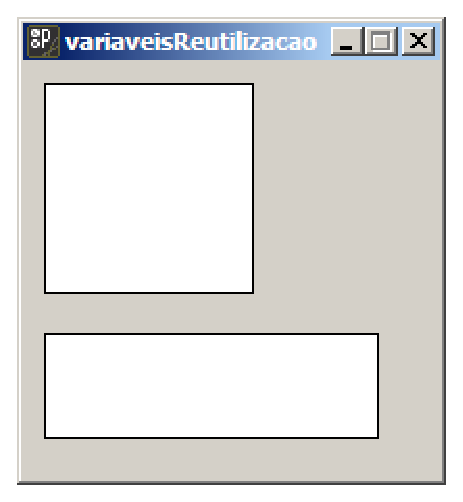
\includegraphics[width=4cm]{images/variaveisReutilizacao.eps}
\end{center}
\begin{lstlisting}[caption=Reutilização de variáveis, label=exe:variaveisReutilizacao]
int larguraRectangulo;
int alturaRectangulo;

size(200, 200); //define a largura da janela: 200x200

larguraRectangulo = 100; // largura 100 para o primeiro rectangulo.
alturaRectangulo = 100;  // altura 100 para o primeiro rectangulo.
rect(10, 10, larguraRectangulo, alturaRectangulo); // desenha o rectangulo na posicao 10, 10.

larguraRectangulo = 160; // largura 160 para o segundo rectangulo.
alturaRectangulo = 50;   // altura 50 para o segundo rectangulo.
rect(10, 130, larguraRectangulo, alturaRectangulo); // desenha o rectangulo na posicao 10, 130.
\end{lstlisting}
\end{minipage}

No programa do exemplo anterior podemos ver que as variáveis declaradas são utilizadas várias vezes no nosso programa.


\section{Guardar na Gaveta (Atribuição)}
As variáveis apenas têm utilidade se lhes podermos alterar e ler o seu conteúdo. Para colocarmos um valor%
\footnote{Colocar um valor numa variável é \emph{atribuir} um valor a essa variável.}
 numa variável basta escrever numa linha o nome da variável seguido do símbolo ``='' (igual), seguido do valor que pretendemos atribuir e terminando com ``;'' (ponto e vírgula).
Ou seja, algo do género (os programas anteriores já tinham instruções destas)%
\footnote{Neste programa, faço uma atribuição de um valor decimal a uma variável. Em Processing, as casas decimais são separadas por um ``.'' (ponto) e não por ``,'' (vírgula).}%
:
\begin{lstlisting}
float minhaVariavel; //primeiro temos sempre de declarar a variável.

minhaVariavel = 102.4; //atribuir o valor 102.4
\end{lstlisting}


Uma variável guarda sempre um valor durante o programa, mas esse valor pode ser alterado em qualquer ponto do programa pela atribuição, pelo que podemos fazer com que uma variável guarde valores diferentes em momentos diferentes do programa:
\begin{lstlisting}
int x;
int y;

x = 0;
y = 0;
point(x, y);

x = 2;
y = 3;
point(x, y);
\end{lstlisting}
Este programa utiliza a mesma instrução duas vezes -- \texttt{point(x, y)} -- mas em momentos diferentes no programa, pelo que o resultado da execução das duas instruções é diferente.
Na primeira, \texttt{point(x, y)} da linha 6, pode ser substituida por \texttt{point(0, 0)} (\texttt{x} e \texttt{y} têm ambas o valor zero, neste ponto).
Na segunda, \texttt{point(x, y)} da linha 10, pode ser substituida por \texttt{point(2, 3)} (neste ponto \texttt{x} tem o valor 2 e \texttt{y} tem o valor 2). 
O resultado deste programa seria o desenho de dois pontos (pixeis) no ecrã: um na posição (0, 0) e outro na posição (2, 3).


\subsection{Inicialização}
Um conceito associado com a declaração de variáveis é a \emph{inicialização} de variáveis. Antes de podermos utilizar o valor de uma variável, é necessário que essa variável contenha algum valor. Caso contrário, qual seria o resultado? Observem o programa seguinte:
\begin{lstlisting}
int x;
int y;

point(x, y);
\end{lstlisting}
Em que posição do ecrã irá ser desenhado o ponto?

Se responderam (0, 0), estão errados :).

O valor zero (0) parece o mais óbvio, mas de facto, em Processing%
\footnote{Em algumas linguagens de programação, é, de facto, o zero! Nessas linguagens as variáveis são inicializadas automaticamente com o valor zero, se o programador não as inicializar.}%
, não é assim. Se experimentarem correr este programa no Processing irão deparar-se com um erro de compilação. Em Processing, não é possível utilizar uma variável que não tenha sido inicializada, ou seja, uma variável à qual ainda não tenha sido feita uma atribuição.

Para corrigir o programa anterior teriamos então de inicializar as duas variáveis:
\begin{lstlisting}
int x;
int y;

x = 0;
y = 4;
point(x, y);
\end{lstlisting}
Reparem que não é necessário inicializar uma variável com o valor zero. Podemos inicializa-las com qualquer valor que faça sentido no nosso programa!

\subsection{Combinar Declaração com Atribuição}
Uma vez que, depois de declarar uma variável, é obrigatório inicializá-la, o Processing fornece-nos uma forma de fazer estes dois passos mais rapidamente: combinando a declaração com a inicialização. 
O exemplo seguinte mostra como se faz isto:
\begin{lstlisting}
int x = 0;
int y = 4;

point(x, y);
\end{lstlisting}

\section{Visibilidade}
É possível fazer a declaração de variáveis em qualquer ponto do programa, embora seja boa prática fazê-lo no início do programa.
É possível mesmo declarar variáveis dentro de métodos%
\footnote{Vamos ver num capítulo mais à frente exactamente o que são métodos. Para já, podemos considerá-los como pedaços de código com nome, ou seja, blocos de código que podem ser chamados (executados) pelo nome.}%
:
\begin{lstlisting}
int x; //variável global
int y; //variável global

void setup() {
    int z = 4; //variável local ao setup()
	  
    size(200, 200);
    x = 0;
    y = 0;
}

void draw() {	
    point(x, y);
}
\end{lstlisting}
O exemplo anterior, utiliza três variáveis: \texttt{x}, \texttt{y} e \texttt{z}. As primeiras duas estão declaradas no início do programa. A variável \texttt{z} está declarada dentro do método \texttt{setup()}.

Dizemos que as variáveis \texttt{x} e \texttt{y} são variáveis globais e a variável \texttt{z} é uma variável local.
As variáveis globais são variáveis que são visíveis, isto é, podem ser utilizadas, em qualquer ponto do programa. No caso do exemplo, as variáveis \texttt{x} e \texttt{y}, apesar de declaradas fora do \texttt{draw()}, são utilizadas lá dentro.

As variáveis locais apenas podem ser utilizadas dentro do bloco onde foram declaradas: a variável \texttt{z} foi declarada dentro do bloco correspondente ao método \texttt{setup()} pelo que apenas pode ser utilizada dentro desse método.
Se tentássemos utilizá-la noutro sítio, como por exemplo:
\begin{lstlisting}
int x; //variável global
int y; //variável global

void setup() {
    int z = 4; //variável local ao setup()	  
    size(200, 200);
    x = 0;
    y = 0;
}

void draw() {	
    point(x, y);
	
    point(z, 5); //erro! 'z' só é conhecida dentro de setup() e nao draw()
}
\end{lstlisting}
Este programa não iria compilar: a variável \texttt{z} utilizada em \texttt{draw()} não é conhecida.

Então porque não utilizar sempre variáveis globais? 

As variáveis globais consomem memória (afinal, as variáveis \textbf{são} memória) do computador durante toda a execução do programa. As variáveis locais apenas consomem memória enquanto o bloco está a executar. Para além disso, no caso de programas muito complexos, tornar-se-ia confuso para o programador ter uma lista muito grande de variáveis globais, quando algumas apenas são utilizadas dentro de um método!

Assim, se apenas precisarmos de uma variável para contas intermédias dentro de um método, devemos declarar essa variável local a esse método.

%--------------
O lugar onde declaramos as variáveis no nosso programa: corpo principal ou dentro dos métodos, pode ser visto como uma estrutura de caixas dentro de caixas. 
%--------------
\section{Instruções}
Já vimos, até aqui, que podemos atribuir valores a variáveis. No entanto, as instruções de atribuição que vimos até agora foram todas muito básicas. 

O valor que atribuimos a uma variável pode ser uma valor literal ou o resultado da avaliação de uma expressão com variáveis, métodos, etc.
\emph{Literal}, em programação, é um valor codificado directamente na instrução. Por exemplo, na instrução
\begin{lstlisting}
x = 10;
\end{lstlisting}
o valor 10 é um literal. 

\subsection{Operadores Aritméticos} 
Soma (+); subtracção (-); multiplicação (*); divisão(/); resto da divisão (\%). Os operadores aritméticos podem ser usados sobre dados do tipo inteiro ou real. 

Os operadores aritméticos podem ser combinados:
\begin{lstlisting}
int x = 2;
int y;
y = 2 + x * 4;
\end{lstlisting}

É preciso ter cuidado, no entanto, com a ordem com que as operações são efectuadas. No caso do exemplo anterior que operação é efectuada primeiro? $2 + x$, ou $x * 4$?
Para resolver este problema existe a noção de precedência das operações. No caso das operações aritméticas, a multiplicação,
divisão e resto da divisão têm maior precedência do que a soma e subtracção, o que significa que são efectuadas primeiro. 
Se a precedência das operações for igual, então as operações são feitas da esquerda para a direita (associatividade à esquerda).

Se quisermos que determinada operação tenha precedência sobre outra podemos utilizar os parêntesis:
\begin{lstlisting}
int y;

y = 2 / (x + 4);
\end{lstlisting}
Neste caso, a soma irá ser efectuada antes da divisão.

Quando temos expressões muito complexas, é boa prática utilizar os parêntesis, mesmo que o problema da precedência
não se coloque. A utilização de parêntesis facilita a leitura da expressão.

\subsection{Uma Operação Complicada! (Instruções Complexas)}

Para além das expressões matemáticas podemos também utilizar nas instruções chamadas a métodos%
\footnote{Em programação existem dois tipos de métodos: métodos que devolvem um valor e métodos que não devolvem valor nenhum. Nas expressões de atribuição podemos utilizar métodos que retornam valores.}%
:
\begin{lstlisting}
int x = 0;
int y = 6;

x = y * 5 + sqrt(16);
\end{lstlisting}
O método \texttt{sqrt(16)} devolve o valor da raiz quadrada de 16. Quando o programa chegar à expressão de atribuição irá substituir automaticamente os valores das variáveis e métodos pelos seus valores actuais. Ou seja, a expressão \texttt{y * 5 + sqrt(16)} é o mesmo que \texttt{6 * 5 + 4} que será igual a \texttt{34}.

Este processo de substituição pode ser utilizar em qualquer nível de profundidade:
\begin{lstlisting}
int x = 0;
int y = 6;

x = y * 5 + sqrt(y*6+sqrt(169);
\end{lstlisting}
A expressão \texttt{y * 5 + sqrt(y*6+sqrt(169)} será substituída recursivamente por \texttt{6 * 5 + sqrt(6*6+13)} e depois 
por \texttt{30 + sqrt(49)}, depois por \texttt{30 + 7} e finalmente por \texttt{37}.

\section{Exercícios}
\begin{enumerate}
\item \label{exe:3_tipos}
* Indique qual o melhor tipo de variável para cada uma das seguintes situações:
\begin{enumerate}
\item A idade de uma pessoa.
\item O preço de um artigo de supermercado.
\item A nota final de um aluno à cadeira de Programação Multimédia.
\item Armazenar uma pergunta de um teste.
\item O peso de todos os elementos de uma corporação de bombeiros.
\item A cor de cada pixel de uma imagem digital.
\item As alíneas deste conjunto de problemas.
\item O número do BI.
\item Os números de telefone dos seus contactos do telemóvel.
\item Os preços de um determinado artigo de supermercado ao longo dos 12 meses do ano.
\item A sua média de entrada na faculdade.
\end{enumerate}

\item \label{exe:3_declaracao}
* Escreva as instruções de declaração das variáveis da secção anterior.

\item \label{exe:3_1}
* Crie um programa em Processing que desenhe 5 linhas em posições diferentes alterando apenas os valores de variáveis. Ou seja a instrução para desenhar deve ser sempre \texttt{line(x0, y0, x1, y1);}. Altere apenas os valores das variáveis.

\item  \label{exe:3_2} \label{ps:linhaAnimada}
* Crie um programa que anime uma linha no ecrã. Irá ter de utilizar o método \texttt{draw()} (veja um dos exemplos e altere).
Pense nas variáveis que terá de utilizar, onde as deverá inicializar e onde as deverá actualizar. Não faz mal se a sua linha desaparecer do ecrã a certa altura, mas pense no que teria de fazer para evitar isso.

\item  \label{exe:3_3}
* Diga o que está mal no programa seguinte:
\begin{lstlisting}
int largura;

void setup() {
    size(200, 200);
    
    largura = 100;
    altura = 100;
}

void draw() {
    rect(10, 10, largura, altura);
}
\end{lstlisting}
Corrija-o.
\end{enumerate}

\chapterimage{band1.png}
\chapter{Condições}\label{cap:seleccao}

Na nossa vida diária, a maior parte das acções que efectuamos estão sujeitas a determinadas condições para poderem ser realizadas. Vamos à aula de Programação Multimédia,  \textbf{se} quisermos ser os melhores a programar;) vamos à praia se não estiver a chuver; se tivermos fome, comemos; se gostarmos da comida, vamos à cantina, senão...vamos a outro lado; etc.

Também em programação necessitamos de executar acções condicionalmente, i.e., se determinadas circunstâncias se verificarem. 
Ao processo de execução condicional de determinadas secções de código do programa chamamos \emph{controlo de fluxo}.

Podemos controlar o fluxo do programa, i.e., que secções de código executam, recorrendo a estruturas de controlo
de fluxo. Essas estruturas são duas: \texttt{if} e \texttt{switch}.


\section{Se Isto Então Aquilo (\texttt{if})}
\begin{figure}[!ht]
	\centering
		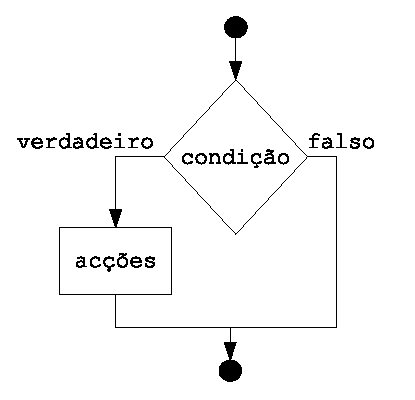
\includegraphics[width=5cm]{images/se-entao.eps}
	\caption{\texttt{if else} -- Diagrama de Fluxo}
	\label{fig:se-entao}
\end{figure}
A estrutura \texttt{if}, permite-nos executar condicionalmente um conjunto de instruções.
Na sua forma mais básica, a estrutura reduz-se a:
\begin{lstlisting}
if (<condição>) {
    [acções]
}
\end{lstlisting}

Por exemplo:
\begin{lstlisting}
int x;

x = 5;

if (x > 10) {
    print("X é maior do que 10.");
}
\end{lstlisting}
Neste caso, a frase ``X é maior do que 10'' apenas é escrita se
o valor de \texttt{x} for superior a 10. Caso contrário a instrução
de escrita é simplesmente ignorada. A Figura~\ref{fig:se-entao} mostra o diagrama de fluxo da estrutura
\texttt{if}. Esta estrutura é composta por duas partes fundamentais:
\begin{description}
\item[condição] 
A condição é a situação que queremos testar. No caso do exemplo, queriamos saber se a variável \texttt{x} tinha um valor superior a 10.

\item[acções]
São as instruções que queremos executar se a condição for \textbf{verdadeira}. As instruções a executar são delimitadas por duas chavetas (``\{'' e ``\}''). As chavetas, em Processing, servem para delimitar um \emph{bloco de código}. No caso do \texttt{if}, o bloco de código é um conjunto de instruções (podemos ter várias instruções) executado se a condição for verdadeira.
\end{description}

E se quisermos testar também a condição inversa? Ou seja, falsa?

Uma das opções seria (no caso do exemplo anterior)%
\footnote{A condição inversa de ``x maior do que 10'' é ``x menor ou igual a 10''.}%
:
\begin{lstlisting}
int x;

x = 5;

if (x > 10) {
    print("X é maior do que 10.");
}
if (x <= 10) {
    print("X é menor ou igual a 10.");
}
\end{lstlisting}
Neste exemplo conseguimos determinar se ``x maior do que 10'' e também se ``x menor ou igual a 10''. No entanto, o Processing, fornece-nos uma forma mais rápida (em termos de escrita de código) de conseguir isto:
\begin{lstlisting}
int x;

x = 5;

if (x > 10) {
    print("X é maior do que 10.");
} else {
    print("X é menor ou igual a 10.");
}
\end{lstlisting}

A \emph{keyword} \texttt{else} serve para executar um conjunto de instruções caso a condição do \texttt{if} seja falsa. De novo, o conjunto de instruções a executar é delimitado por chavetas.
O diagrama desta estrutura (\texttt{if else}) é apresentado na Figura~\ref{fig:se-entao-senao}.

\begin{figure}[!ht]
	\centering
		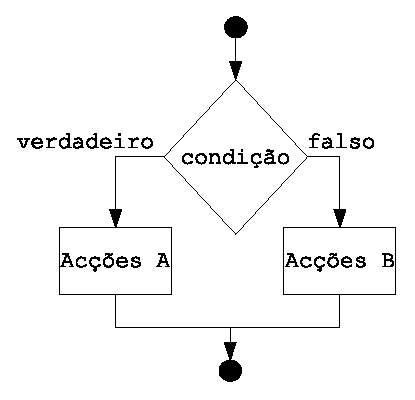
\includegraphics[width=5cm]{images/se-entao-senao.eps}
	\caption{\texttt{if else} -- Diagrama de Fluxo}
	\label{fig:se-entao-senao}
\end{figure}

A estrutura \texttt{if} pode ser utilizada em ``cascata'', i.e., podemos testar várias condições consecutivamente:
\begin{lstlisting}
int x;

x = 5;

if (x > 10) {
    print("X é maior do que 10.");
} else if (x > 5) {
    print("X é maior do que 5.");
} else if (x > 1) {
    print("X é maior do que 5.");
} else {
    print("X é menor ou igual a 1.");
}
\end{lstlisting}


\begin{figure}[ht]
	\centering
		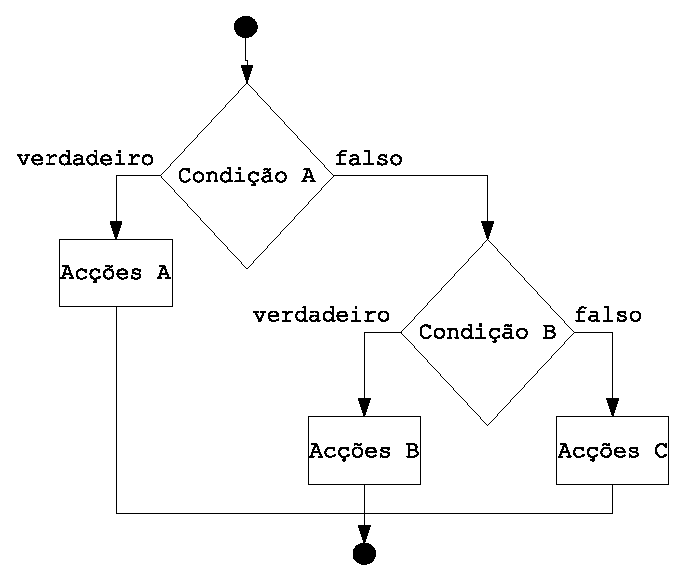
\includegraphics[width=8cm]{images/se-entao-senao-se-senao.eps}
	\caption{\texttt{if else if} -- Diagrama de fluxo}
	\label{fig:se-entao-senao-se-senao}
\end{figure}

Nesta variante, as condições são testadas sequencialmente. Se alguma das condições for
satisfeita, as acções associadas serão executadas e o programa sairá da estrutura, ou seja,
apenas um dos conjuntos de instruções pode ser executado. A Figura~\ref{fig:se-entao-senao-se-senao}
mostra o diagrama de fluxo correspondente.

Obviamente, que o conjunto de instruções executado caso a condição seja verdadeira (ou falsa) pode conter ele mesmo outras estruturas \texttt{if} (o \texttt{if} é uma instrução como outra qualquer):
\begin{lstlisting}
int x;
int y;

x = 5;
y = 7;

if (x > 10) {
    print("X é maior do que 10.");
    if (y > 5) {
        print("Y é maior do que 5.");
    }
} 
\end{lstlisting}
Neste exemplo, escrevemos a mensagem \emph{``X é maior do que 10.''} se \texttt{x} for maior do que 10 e escrevemos a mensagem 
\emph{``Y é maior do que 5.''} se \texttt{x} for maior do que 10 e ao mesmo tempo \texttt{y} for maior do que 5.

\section{Comutar (\texttt{switch})}

\begin{figure}[!h]
	\centering
		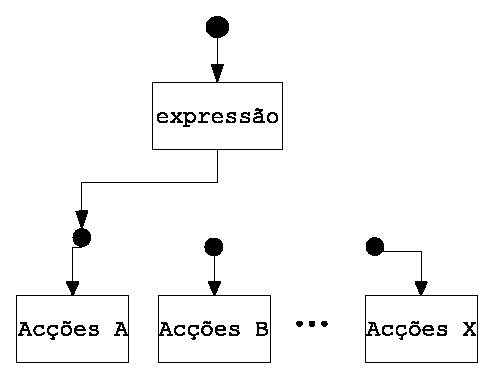
\includegraphics[width=6cm]{images/comuta.eps}
	\caption{\texttt{switch} -- Diagrama de fluxo}
	\label{fig:comuta}
\end{figure}

A estrutura \texttt{switch} é uma forma mais prática, nalguns casos, de escolher um
caminho de entre vários possíveis. É utilizado um valor inteiro para decidir
qual o caminho a executar:
\begin{lstlisting}
int x;

switch (x) {
    case 1: 
        /* instruções a executar se x for igual a 1	*/
        break;
	
    case 2: 
        /* instruções a executar se x for igual a 2	*/
        break;
	
    case 4: 
        /* instruções a executar se nenhum dos anteriores for executado	(opcional) */
        break;	    
}
\end{lstlisting}

O \texttt{switch} é composto por duas secções:
\begin{description}
\item[expressão de teste] 
A expressão de teste é normalmente uma variável do tipo \texttt{int}. Por exemplo, se tivermos uma variável que representa uma opção do utilizador, que pode ir de 1 a 5, podemos ter acções diferentes para cada opção.
	
\item[acções para para caso]
São as instruções a executar se a variável tiver o valor do caso actual. As instruções devem sempre terminar com a instrução \texttt{break}%
\footnote{A keyword \texttt{break} é utilizada para ``partir'' o fio de execução do programa nalgumas situações. No caso do \texttt{switch}, o \texttt{break} faz com que o programa saia da estrutura \texttt{switch}.}%
.
\end{description}



\section{Opero...Se... (Operadores Condicionais)}

Até agora vimos apenas um tipo de condição ``x \textbf{maior do que}...''. No entanto, existem mais condições que podemos testar:
\begin{itemize}
\item Igual a ($==$)%
\footnote{O operador condicional de ``igual a'' é o símbolo $==$ para se distinguir do operador de atribuição $=$ de variáveis.}%
;
\item Maior do que ($>$);
\item Menor do que ($<$);
\item Maior ou igual a ($>=$);
\item Menor ou igual a($<=$);
\item Diferente de ($!=$)
\end{itemize}

Os símbolos entre parentesis são os chamados \emph{operadores condicionais}.
Os operadores condicionais podem ser usados sobre dados de vários tipos (inteiros, reais, lógicos). O resultado da operação é um valor lógico: verdadeiro ou falso.

Os operadores condicionais são utilizados sobretudo no controlo de fluxo do programa e nas condições 
de paragem dos ciclos (explicado no capítulo seguinte). No entanto podemos atribuir o resultado de uma operação
condicional a uma variável lógica:
\begin{lstlisting}
boolean maior;

maior = 1 > 3;
\end{lstlisting}
Neste caso, o valor de \texttt{maior} seria \texttt{false}%
\footnote{A \emph{keyword} \texttt{false} é um valor especial do Processing que pode ser atribuido a variáveis lógicas. De igual modo, existe a \emph{keyword} \texttt{true}.}%
.

\subsection{Lógicos} 
Nos exemplos com condições que vimos até agora, todas as condições eram simples: ``x maior do que 10'', ``y maior do que 5'', etc. No entanto, as condições a testar podem ser bastante mais complexas.

Na vida real, pensamos muitas vezes coisas do género: ``se o FCP ganhar o jogo \textbf{e} o SLB perder, o FCP ganha o campeonato'', ou ``se o SCP ganhar \textbf{ou} o SLB empatar, o FCP perde o campeonato'' ou ``se eu \textbf{não} passar no exame de condução, vou ter de o repetir''.
Todas estas situações representam condições complexas que não são mais do que a conjugação de várias condições simples: ``o FCP ganhar o jogo'', ``o SLB perder o jogo'', ''passar no exame de condução'', etc. Estas condições simples, são ligadas através do que se designa, em programação, por \emph{operadores lógicos}: \textbf{e}, \textbf{ou} e \textbf{não}. 

Os operadores condicionais servem ligar condições simples, de modo a criar condições mais complexas. O valor da condição complexa resultante (verdadeira ou falsa) depende do valor de cada condição simples.

Os símbolos utilizados em Processing para representar estes operadores são os seguintes:
\begin{center}
\begin{tabular}{lll}
Operador & Símbolo & Descrição\\
\hline
	\textbf{e} &\texttt{\&\&} &dois ``\&'' (e comercial).\\
	\textbf{ou} &\texttt{||} &dois ``|'' (\emph{pipeline} -- símbolo que se encontra\\
	& & por cima da barra invertida ``$\backslash$'' no teclado).\\
	\textbf{não} &\texttt{!} &um ``!'' (ponto de exclamação).\\
\end{tabular}
\end{center}

Os operadores lógicos (``ou'', ``e'', ``não'') operam sobre dados lógicos. Os operadores ``ou'' e
``e'' são operadores binários (operam sobre dois operandos); o operador ``não'' é um operador unário. As tabelas 
de verdade%
\footnote{Uma \emph{tabela de verdade} é uma tabela que indica o resultado da conjugação de um operador lógico com todos os valores possíveis dos operandos.}
 de cada operador são as seguintes:
\begin{center}
\begin{tabular}{c|c|c}
\multicolumn{3}{c}{\texttt{||} -- (``ou'')}\\
\hline
A & B & A \texttt{||} B\\
\hline
\texttt{false} & \texttt{false} & \texttt{false}\\
\texttt{false} & \texttt{true} & \texttt{true}\\
\texttt{true} & \texttt{false} & \texttt{true}\\
\texttt{true} & \texttt{true} & \texttt{true}\\
\end{tabular}
\end{center}

\begin{center}
\begin{tabular}{c|c|c}
\multicolumn{3}{c}{\texttt{\&\&} -- (``e'')}\\
\hline
A & B & A \texttt{\&\&} B\\
\hline
\texttt{false} & \texttt{false} & \texttt{false}\\
\texttt{false} & \texttt{true} & \texttt{false}\\
\texttt{true} & \texttt{false} & \texttt{false}\\
\texttt{true} & \texttt{true} & \texttt{true}\\
\end{tabular}
\end{center}

\begin{center}
\begin{tabular}{c|c}
\multicolumn{2}{c}{\texttt{!} -- (``não'')}\\
\hline
A & \texttt{!}A\\
\hline
\texttt{false} & \texttt{true}\\
\texttt{true} & \texttt{false} \\
\end{tabular}
\end{center}

Uma vez que o resultado de uma operação condicional é um valor lógico, podemos combinar operações condicionais
e lógicas:
\begin{lstlisting}
boolean maisAltoEMaisVelho = (idadeJoao > idadeAna) e (alturaJoao > alturaAna);
\end{lstlisting}
Neste caso \texttt{maisAltoEMaisVelho} será \texttt{true} apenas se a idade do João
for superior à idade da Ana e se ele for também mais alto. A utilização dos parêntesis, neste
caso, não era absolutamente necessária porque os operadores condicionais têm precedência
sobre os operadores lógicos. No entanto, a sua utilização facilita a leitura do código.

\section{Um Exemplo Prático}
Tendo conhecimentos destes novos operadores -- condicionais e lógicos -- podemos escrever programas mais complexos.

O exemplo seguinte é um programa que consiste num quadrado branco que sobe e desce no ecrã. A única informação (variáveis) que precisamos de manter é a posição vertical actual do quadrado e a velocidade a que se desloca (quantos pixeis se mexe de cada vez). 
\begin{center}
	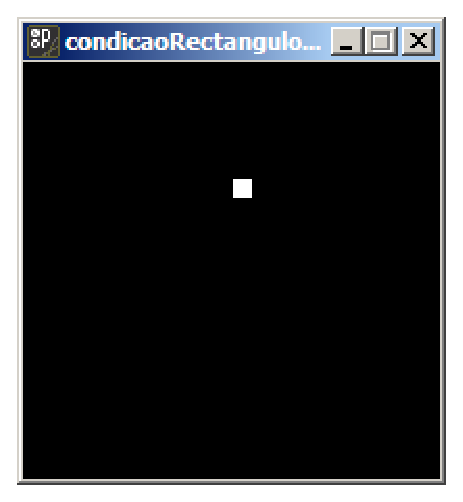
\includegraphics[width=4cm]{images/condicaoRectanguloCimaBaixo.eps}
\end{center}
\begin{lstlisting}[caption=Testar a posição vertical de um rectângulo, label=exe:condicaoRectanguloCimaBaixo]
int y;          //a posição do quadrado
int velocidade; //a velocidade (pode ser negativa)

void setup() {
    size (200, 200);
    
    y = 0;
    velocidade = 5;
}


void draw() {
    background(0);       //limpar o ecra
    
    rect(100, y, 10, 10); //desenhar o rectangulo na posicao vertical y
    
    y = y + velocidade;   //actualizar a posicao
        
    if (y > 200) {        // se o rectangulo passou o fundo do ecra, inverter a velocidade
        velocidade = -5;
    }
    if (y < 0) {          // se o rectangulo passou o cimo do ecra, inverte a velocidade
        velocidade = 5;
    }
}
\end{lstlisting}
O rectângulo é desenhado com a instrução \texttt{rect(100, y, 10, 10)}%
\footnote{A instrução \texttt{rect()} precisa de quatro parâmetros: a posição x e y e a largura e altura do rectângulo.}
de forma que o rectângulo é desenhado na posição vertical dada pela variável \texttt{y}.
Uma vez que a variável \texttt{y} é actualizada com o valor da velocidade, isto faz com que o rectângulo seja desenhado sempre numa posição diferente, dando a ilusão de movimento contínuo.

Para verificarmos se o rectângulo bateu numa das paredes (limites da janela, inferior ou superior) basta-nos testar a posição vertical. Uma vez que sabemos qual a dimensão da janela (200x200), sabemos que se a posição \texttt{y} for superior a 200, então o rectângulo bateu na parede inferior (lembrem-se que o y ``cresce'' para baixo). De igual modo se a posição for inferior a 0, bateu na parede superior.



\section{Exercícios}
\begin{enumerate}
	
	\item \label{exe_4_operadores} 
	* Determine o resultado lógico das seguintes expressões, sabendo que ($a = 13, b = 2, c = 3, n = verdadeiro, p = falso$):
\begin{enumerate}
\item $a == b$ 
\item $a < b$
\item $a > b > c$
\item $!(a > b)$
\item $! !(a > b)$
\item $(a > b) \&\& (b > c)$
\item $!((a > b) \&\& (b > c))$
\item $(!(a > b)) \&\& (b > c)$
\item $n || p$
\item $(a>b) \&\& p$
\item $!((a>b) \&\& p)$\item Nas expressões anteriores, em que o resultado é \emph{falso}, determine valores para $a$, $b$ e $c$ de
modo a torná-las \emph{verdadeiro}.
\end{enumerate}

\item \label{exe_4_fluxo}
* Escreva os programas para resolver os seguintes problemas:
\begin{enumerate}

\item Determinar a média de dois valores inteiros. Escrever o valor da média
se esta for superior a 100. Assuma que os valores estão armazenados nas variáveis $a$ e $b$.

\item Determinar se um valor é positivo, negativo ou zero. Assuma que o valor está armazenado na variável $a$.

\item Determinar se um valor (gerado aleatoriamente) é par ou ímpar. 

\item Determinar, de entre dois valores, o maior e o menor (ou se são iguais). Por exemplo, se os dois valores forem 4 e 2, o 
programa deve escrever: 
\begin{lstlisting}
"O maior valor é 4"
"O menor valor é 2"
\end{lstlisting}
Se os valores forem 2 e 2, deve escrever:
\begin{lstlisting}
"Os valores são iguais"
\end{lstlisting}
Assuma que os valores estão armazenados nas variáveis $a$ e $b$.

\item Determinar se uma coordenada ($x, y$), introduzida pelo utilizador, está dentro de um rectângulo definido definido pelos seus cantos superior esquerdo ($x0, y0$) e inferior direito ($x1, y1$). O programa deve apresentar o resultado ao utilizador: ``A coordenada está dentro do rectângulo'' ou ``A coordenada está fora do rectângulo''. \label{xpto}

\item Determinar o máximo de três valores. Assuma que os valores estão armazenados nas variáveis $a$, $b$ e $c$.

\item Determinar o máximo de cinco valores.
Assuma que os valores estão armazenados nas variáveis $a$, $b$, $c$, $d$ e $e$.
\end{enumerate}

	\item \label{exe:4_1}
	* Altere o Projecto \ref{ps:linhaAnimada} do capítulo anterior, de modo a que a linha se mantenha sempre dentro do ecrã e sempre animada.
\end{enumerate} 

\chapterimage{band1.png}
\chapter{Iteração}\label{cap:iteraccao}

A maior parte dos programas repetem várias vezes as mesmas operações sobre os mesmos dados ou sobre dados
diferentes. 
Muitas acções que realizamos na vida real são, de facto, a repetição de uma acção mais básica. Por exemplo, subir escadas: a acção mais básica é subir um degrau; esta operação é repetida até chegarmos ao final das escadas. Poderiamos pensar que a acção básica não é a mesma repetida, afinal, não subimos sempre o mesmo degrau! Mas nestes casos, o que interessa é que o conjunto de acções que a pessoa efectua para subir um degrau: levantar a perna, apoiar o pé, elevar o corpo e apoiar o outro pé, são sempre os mesmos independentemente do degrau estar mais acima ou mais abaixo.

Também em programação acontece frequentemente necessitarmos de repetir várias vezes a mesma acção, um determinado número de vezes, ou enquanto determinada condição for verdadeira.

Para repetirmos um conjunto de operações utilizamos as chamadas instruções de \emph{iteração}, ou \emph{ciclos}.

Existem duas classes de ciclos: ciclos que executam um número pré-determinado de vezes e ciclos que executam enquanto determinada condição não for satisfeita. Estas classes de ciclos têm analogias com situações da vida real. Na situação de ``subir a escada'', normalmente não sabemos à partida quantos degraus vamos ter de subir, mas sabemos que temos de continuar a subir degraus enquanto eles não acabarem, ou enquanto não chegarmos ao nosso piso -- este seria um ciclo que executa enquanto determinada condição não for satisfeita. Numa outra situação, por exemplo no caso em que vamos comprar laranjas ao supermercado, normalmente sabemos quantas laranjas vamos querer comprar. Neste caso colocamos laranjas no saco até chegarmos ao número pretendido -- este ciclo executa um número pré-determinado de vezes.

Para a primeira classe de ciclos existem duas variantes em programação: o ciclo \texttt{while} -- executa zero ou mais vezes, enquanto uma condição for verdadeira; e o ciclo \texttt{do} -- executa uma ou mais vezes, enquanto uma condição for verdadeira; 

Para a segunda classe de ciclos existe o ciclo \texttt{for} -- utilizado principalmente para iterar um número pré-determinado de vezes; 


\section{\texttt{while}}
A Figura~\ref{fig:enquanto} mostra o diagrama de fluxo do ciclo \texttt{while}.
\begin{figure}[!h]
	\centering
		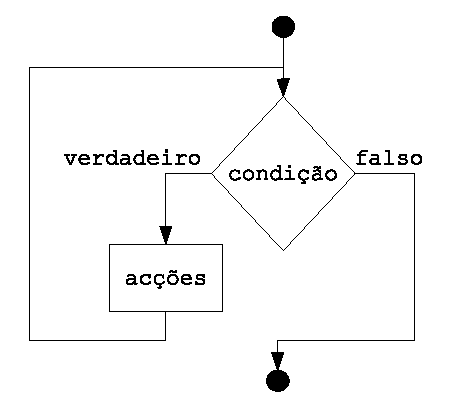
\includegraphics[width=5cm]{images/enquanto.eps}
	\caption{\texttt{while} -- diagrama de fluxo}
	\label{fig:enquanto}
\end{figure}

A sintaxe deste ciclo é a seguinte:
\begin{lstlisting}
while (<condição>) {
    <acções>
}
\end{lstlisting}

Quando o programa chega à primeira linha do ciclo, a condição é testada. Se a condição for verdadeira, então o programa segue para a primeira linha das acções. Quando chegar à última linha das acções, o programa volta automaticamente à primeira linha do ciclo e testa novamente a condição. Se a condição for falsa, então o programa segue para a instrução a seguir ao final do ciclo. Uma vez que a condição é testada no início do  ciclo, pode acontecer que o ciclo não execute nenhuma vez: se a condição for falsa logo da primeira vez.

O exemplo seguinte exemplifica o uso deste ciclo para escrever os números de 0 a 10:
\begin{lstlisting}
int i = 0;
while (i <= 10) {
    print(i);
    i = i + 1;
}
\end{lstlisting}
Neste exemplo, a condição para execução do ciclo é a variável \texttt{i} ser menor ou igual a 10. Se isto for verdade, então o programa escreve o valor de \texttt{i} -- com a instrução \texttt{print()} -- e aumenta o valor da variável. No exemplo, a variável \texttt{i} foi inicializada a zero. Se a inicializassemos com um valor superior a 10, o ciclo não executava nenhuma iteração%
\footnote{Uma \emph{iteracção} é uma execução das acções de um ciclo.}%
:
\begin{lstlisting}
int i = 15;
while (i <= 10) {
    print(i);
    i = i + 1;
}
\end{lstlisting}
Neste caso, a condição é falsa logo à partida.


\section{\texttt{do}}
O ciclo \texttt{do} é uma variante do ciclo anterior.
A Figura~\ref{fig:fazer} mostra o diagrama de fluxo do ciclo \texttt{do}.
\begin{figure}[!h]
	\centering
		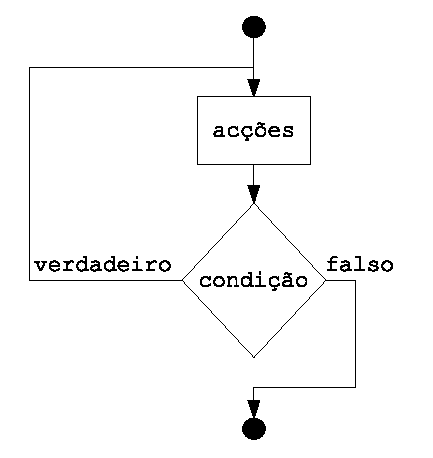
\includegraphics[width=5cm]{images/fazer.eps}
	\caption{\texttt{do} -- diagrama de fluxo}
	\label{fig:fazer}
\end{figure}

A diferença para o ciclo anterior (\texttt{while}) é que, no ciclo \texttt{do}, a condição é testada apenas no final do ciclo. Isto significa que as acções deste ciclo executam sempre, pelo menos uma vez. A sintaxe geral deste ciclo é a seguinte:
\begin{lstlisting}
do {
    <acções>
} while (<condição>);
\end{lstlisting}

Como exemplo de utilização vamos reescrever o exemplo anterior (escrita dos números de 0 a 10) com o ciclo \texttt{do}:
\begin{lstlisting}
int i = 0;
do {
    print(i);
    i = i + 1;
} while (i <= 10);
\end{lstlisting}
Este ciclo executa exactamente o mesmo que o exemplo anterior. No entanto, se agora inicializarmos a variável \texttt{i} a 15, como fizemos anteriormente:
\begin{lstlisting}
int i = 15;
do {
    print(i);
    i = i + 1;
} while (i <=10);
\end{lstlisting}
Verificamos que o programa escreve o valor ``15''. Isto acontece porque o ciclo \texttt{do} executa sempre pelo menos uma vez. Apenas depois da primeira iteracção do ciclo é que a condição é testada.

\section{\texttt{for}}
Este ciclo corresponde à classe de ciclos utilizada para iterar um número pré-determinado de vezes.
O diagrama de fluxo do ciclo \texttt{for} está exemplificado na Figura~\ref{fig:para}.
\begin{figure}[h]
	\centering
		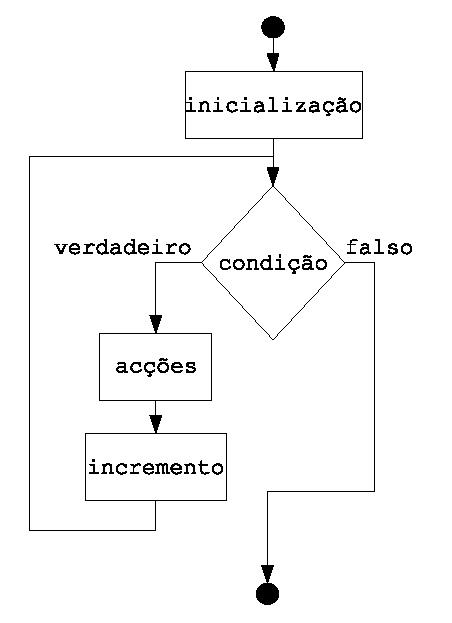
\includegraphics[width=5cm]{images/para.eps}
	\caption{\texttt{for} -- diagrama de fluxo}
	\label{fig:para}
\end{figure}
A sintaxe deste ciclo é um bocado mais complexa do que as anteriores:
\begin{lstlisting}
for (<inicialização>;<condição>;<incremento>) {
    <acções>
}
\end{lstlisting}

O ciclo \texttt{for} utiliza uma variável para contar o número de vezes que já executou. Essa variável pode ser uma qualquer variável numérica do nosso programa que deverá ser inicializada na secção <inicialização> do ciclo. Normalmente utilizamos nomes especiais para estas variáveis: \texttt{i}%
\footnote{O nome \texttt{i} para estas variáveis deve-se ao facto de na maioria das vezes, estas variáveis servirem de \textbf{í}ndices para vectores.}%
, \texttt{j}, \texttt{k}, etc.

Em <condição>, colocamos a condição de paragem do ciclo. Normalmente, esta condição toma a forma de \texttt{i < x;}, em que x é o número de vezes que queremos executar o ciclo.

A secção <incremento> serve para aumentar o valor da variável de forma a avançarmos. Na maior parte das vezes utilizamos: \texttt{i = i + 1;}%
\footnote{Irão ver muitas vezes expressões como \texttt{i++;} em vez de \texttt{i = i + 1;}. As duas são equivalentes.}. 
 para incrementar uma unidade.


Assim para escrevermos os números de 0 a 10, fariamos:
\begin{lstlisting}
int i;
for (i = 0; i <= 10; i = i + 1) {
    print (i);
}
\end{lstlisting}
Reparem que, neste caso, não temos de incrementar a variável no corpo do ciclo. Isto é feito na secção de incremento.



\section{Tipos de variáveis complexos}
Até agora temos vindo a utilizar apenas tipos de variáveis simples. Estas variáveis podem guardar um valor de cada vez -- são ``gavetas'' que apenas podem ter um valor. 

Os vectores são como gavetas sequenciais que podem ser referidas através de um nome e um índice. O nome identifica o conjunto de gavetas, enquanto que o índice identifica a gaveta dentro do conjunto. Deste modo podemos ter vários conjuntos de gavetas com nomes diferentes.
O nome do conjunto de gavetas não é mais do que o nome da variável que definirmos no nosso programa.

Os vectores permitem-nos agrupar dados do mesmo tipo de uma forma mais prática do que se definissemos uma variável para cada valor. Por exemplo, vamos supor que necessitamos de guardar as idades de todos os alunos de uma turma. Os alunos e respectivas idades são:
\begin{center}
\begin{tabular}{ll}
Nome & Idade\\
\hline
Pedro 	& 20 \\
Rui			& 19 \\
Osvaldo & 19 \\
Guilherme	& 20\\
Romão			& 18\\
Ana				& 19\\
Maria			& 18\\
Anacleto	& 20\\
Carlos		& 21\\
António		& 17\\
Osório		& 18\\
Manuela		& 17\\
Ulmira	 	& 18\\
Luís			& 20\\
Tibério		& 19\\
Irina			& 20\\
Mafalda		& 18\\
Emília		& 19\\
Diogo			& 20\\
Isabel		& 19\\
Aleixo		& 20\\
\end{tabular}
\end{center}
Uma possível solução para este problema seria utilizar tantas variáveis como número de alunos:
\begin{lstlisting}
int pedro     = 20;
int rui       = 19;
int osvaldo   = 19;
int guilherme = 20;
int romão     = 18;
int ana       = 19;
int maria     = 18;
int anacleto  = 20;
int carlos    = 21;
int antónio   = 17;
int osório    = 18;
int manuela   = 17;
int ulmira    = 18;
int luís      = 20;
int tibério   = 19;
int irina     = 20;
int mafalda   = 18;
int emília    = 19;
int diogo     = 20;
int isabel    = 19;
int aleixo    = 20;
\end{lstlisting}
E agora, se quisessemos calcular a médias das idades?:
\begin{lstlisting}
float media;

media = (pedro + rui + osvaldo + guilherme + romão + ana + maria + 
        anacleto + carlos + antónio + osório + manuela + ulmira + 
        luís + tibério + irina + mafalda + emília + diogo + isabel + 
        aleixo)/21;
\end{lstlisting}
Como devem ter percebido é muito trabalhoso utilizar tantas variáveis... 

Se reparem bem, todas as variáveis guardam o mesmo tipo de dados: uma idade.
Uma forma mais prática de resolver o problema seria utilizar um vector:
\begin{lstlisting}
int idades[];

idades = new int[21]; 

idades[0]  = 20; // pedro
idades[1]  = 19; // rui  
idades[2]  = 19; // osvaldo
idades[3]  = 20; // guilherme 
idades[4]  = 18; // romão     
idades[5]  = 19; // ana     
idades[6]  = 18; // maria   
idades[7]  = 20; // anacleto  
idades[8]  = 21; // carlos   
idades[9]  = 17; // antónio 
idades[10] = 18; // osório    
idades[11] = 17; // manuela  
idades[12] = 18; // ulmira    
idades[13] = 20; // luís     
idades[14] = 19; // tibério 
idades[15] = 20; // irina 
idades[16] = 18; // mafalda 
idades[17] = 19; // emília 
idades[18] = 20; // diogo 
idades[19] = 19; // isabel 
idades[20] = 20; // aleixo 

int i;
float media = 0;

for (i = 0; i < 21; i = i + 1) {
    media = media + idades[i];
}
media = media/21;
\end{lstlisting}
O programa anterior cria um vector com 21 posições (do tipo \texttt{int}) e inicializa-as com as idades dos alunos.
O ciclo final serve para somar todas as idades (para no fim, calcular a média).

Esta forma de utilizar variáveis é muito mais prática do que a versão anterior, porque é muito mais flexível. Neste caso particular para a inicialização, continua a ser necessário um conjunto de várias linhas de código. Mas todas as outras operações ficam facilitadas pela possibilidade de utilização de um ciclo para percorrer cada posição do vector. Para mostrar mais um exemplo da flexibilidade dos vectores, vamos supor que precisavamos de somar 5 anos a cada idade. Na primeira versão teriamos algo como:
\begin{lstlisting}
pedro     = pedro     + 5;
rui       = rui       + 5;
osvaldo   = osvaldo   + 5;
guilherme = guilherme + 5;
romão     = romão     + 5;
ana       = ana       + 5;
maria     = maria     + 5;
anacleto  = anacleto  + 5;
carlos    = carlos    + 5;
antónio   = antónio   + 5;
osório    = osório    + 5;
manuela   = manuela   + 5;
ulmira    = ulmira    + 5;
luís      = luís      + 5;
tibério   = tibério   + 5;
irina     = irina     + 5;
mafalda   = mafalda   + 5;
emília    = emília    + 5;
diogo     = diogo     + 5;
isabel    = isabel    + 5;
aleixo    = aleixo    + 5;
\end{lstlisting} 

Na versão com vectores bastava:
\begin{lstlisting}
int i;
for (i = 0; i < 21; i = i + 1) {
    idades[i] = idades[i] + 5;
}
\end{lstlisting}

Algumas das linhas de código usadas nos exemplos anteriores precisam de explicação. É isso que vamos ver nas secções seguintes.

\subsection{Declarar e Inicializar Vectores}
A linha
\begin{lstlisting}
int idades[];
\end{lstlisting}
declara um vector de inteiros. Esta linha apenas indica ao programa que vamos utilizar uma variável com o nome \texttt{idades} e que essa variável é um vector. Para o programa poder reservar memória para esta variável falta um pedaço de informação importante: o tamanho do vector, ou seja, quantas posições o vector irá conter.

Para indicarmos ao programa que vamos precisar de x posições temos de utilizar uma \emph{keyword} especial -- \texttt{new}:
\begin{lstlisting}
idades = new int[21]; 
\end{lstlisting}
Com esta linha indicamos ao programa que o nosso vector (\texttt{idades}) precisa de guardar 21 números inteiros.

A sintaxe geral para reservar memória para um vector é a seguinte:
\begin{lstlisting}
nomeVariavel = new tipoVariavel[tamanhoVector];
\end{lstlisting}

Para declarar e reservar espaço para um vector de 100 booleanos, fariamos:
\begin{lstlisting}
boolean passouTeste[];

passouTeste = new boolean[100];
\end{lstlisting}

\subsection{Percorrer Vectores}
Uma das grandes vantagens dos vectores é o facto de podermos realizar a mesma operação sobre cada um dos elementos desse vector. A melhor forma de fazermos isto é através de um ciclo:
\begin{lstlisting}
int posicaoY[] = new int[100];
int i;

for (i = 0; i < 100; i = i + 1) {
    posicaoY[i] = posicaoY[i] + 1;
}
\end{lstlisting}

Basicamente, o que temos de fazer para aceder a uma posição do vector é utilizar a sintaxe \texttt{nomeVector[indice]}.
Por exemplo para aceder à primeira posição%
\footnote{A primeira posição de um vector, em Processing, é a posição 0 (zero). Nalgumas linguagens de programação a primeira posição dos vectores é a posição 1 (um).}%
:
\begin{lstlisting}
int pedro;

pedro = idades[0];
\end{lstlisting}

O valor utilizado como índice do vector pode ser uma variável, ou uma expressão, cujo resultado seja um número inteiro. Por exemplo:
\begin{lstlisting}
int maria;

int i = 2;
maria = idades[i*3];
\end{lstlisting}


\section{Enter The Matrix... (Matrizes)}
Um vector não é mais do que a extensão de uma variável simples, que guarda um valor escalar%
\footnote{Um escalar é um valor simples -- valor representado por um único número.}%
, para uma variável com uma dimensão. Então, porque não estender o vector para uma estrutura bi-dimensional?
De facto, podemos pensar num vector de vectores e o resultado é uma \emph{matriz} -- uma estrutura bi-dimensional -- em forma de tabela.

Uma matriz é em tudo semelhante a um vector, a única diferença é que pode ser percorrido segundo duas direcções: por linha e por coluna. 

A Figura~\ref{fig:variaveis} mostra a relação entre variáveis simples, vectores e matrizes.

\begin{figure}[htbp]
	\centering
		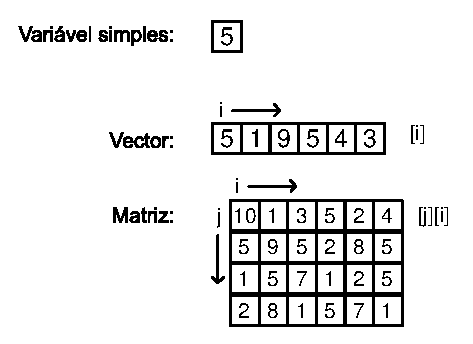
\includegraphics{images/variaveis.eps}
	\caption{Comparação entre variáveis simples, vectores e matrizes}
	\label{fig:variaveis}
\end{figure}

A declaração de uma matriz é feita do seguinte modo:
\begin{lstlisting}
int figura[][];
\end{lstlisting}
Reparem que é muito semelhante à declaração de um vector, a única diferença é que temos mais um par de parentesis rectos: \texttt{[]}.

Da mesma forma temos de reservar espaço em memória. Para isso temos de saber a dimensão da nossa matriz -- número de linhas e número de colunas:
\begin{lstlisting}
figura = new int[<numero de linhas>][<numero de colunas>];
\end{lstlisting}
Supondo que a nossa matriz tem 200 linhas por 300 colunas:
\begin{lstlisting}
figura = new int[200][300];
\end{lstlisting}

\subsection{Percorrer Matrizes}
Uma vez que uma matriz possui mais uma dimensão que um vector, então precisamos de percorrer a matriz segundo duas direcções. Para isto precisamos de dois ciclos: um para percorrer todas as linhas da matriz e outro para percorrer cada linha da matriz:
\begin{lstlisting}
int j; // percorre a matriz na vertical
int i; // percorre na horizontal.

for (j = 0; j < 200; j = j + 1) {
    for (i = 0; i < 300; i = i + 1) {
        print(figura[j][i]);
    }
}
\end{lstlisting}
É necessário ter em atenção a ordem dos índices: \texttt{i} e \texttt{j}. O primeiro índice refere-se sempre ao número da linha, o segundo ao número da coluna (ver Figura~\ref{fig:variaveis}). Tal como nos vectores, os índices começam sempre em 0 (zero).



\section{Dois Exemplos Práticos }

\subsection{Quadrados Saltitantes}
\begin{center}
	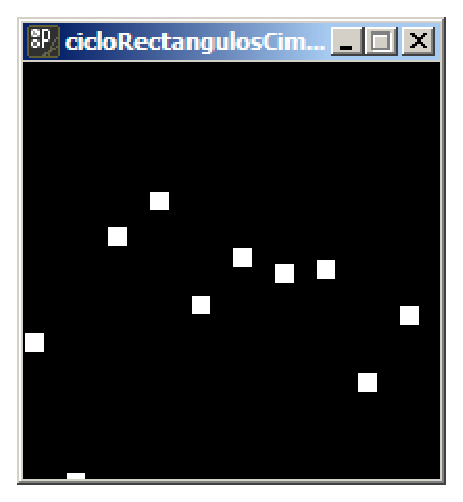
\includegraphics[width=4cm]{images/cicloRectangulosCimaBaixo.eps}
\end{center}
\begin{lstlisting}[caption=Utilização de vectores, label=exe:cicloRectangulosCimaBaixo]
int posicaoY[];    // a posicao de cada quadrado
int velocidadeY[]; // a velocidade de cada quadrado

void setup() {
    size(200, 200);
    
    posicaoY = new int[10];
    velocidadeY = new int[10];
    
    // inicializar a posicao e a velocidade
    for (int i = 0; i < 10; i++) {
        posicaoY[i] = (int)random(200);
        velocidadeY[i] = (int)random(1, 5);
    }
}

void draw() {
    background(0);
    for (int i = 0; i < 10; i++) {
        // desenhar o quadrado na posicao correspondente
        rect(i*20, posicaoY[i], 10, 10);
        
        // actualizar a posicao
        posicaoY[i] = posicaoY[i] + velocidadeY[i];
        if (posicaoY[i] < 0 || posicaoY[i] > 200) {
            velocidadeY[i] = -velocidadeY[i];
        }
    }
}
\end{lstlisting}
O exemplo anterior é uma extensão do Exemplo~\ref{exe:condicaoRectanguloCimaBaixo}.

\subsection{Ruído}
\begin{figure}
	\centering
		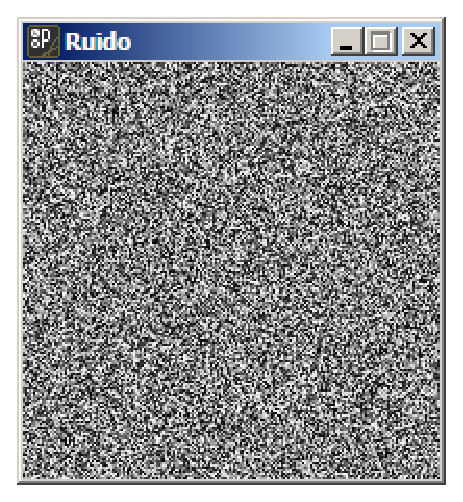
\includegraphics[width=4cm]{images/ruido.eps}
	\caption{Utilização de Matrizes: Ruído}
	\label{fig:ruido}
\end{figure}

\begin{lstlisting}
int ecra[][];

void setup() {
    size(200, 200);
    
    ecra = new int[200][200];
    
    // inicializar a matriz
    for (int i = 0; i < 200; i++) {
        for (int j = 0; j < 200; j++) {
            ecra[i][j] = (int)random(255);
        }
    }
}


void draw() { 
    // desenhar um ponto por cada elemento da matriz
    for (int i = 0; i < 200; i++) {
        for (int j = 0; j < 200; j++) {
            stroke(ecra[i][j]);
            point(j, i);
        }
    }    
}
\end{lstlisting}



\section{Exercícios}

\begin{enumerate}
\item \label{exe_5_ciclos}
* Escreva os programas para resolver os seguintes problemas:
\begin{enumerate}
\item Somar todos os elementos de um vector com 100 inteiros.

\item Somar todos os elementos, positivos, de um vector com 100 inteiros.

\item Somar todos os elementos, maiores do que 10 e inferiores a 20, de um vector com 100 inteiros.

\item Determinar a média dos valores de uma matriz de reais.

\item Dada uma matriz A, de números inteiros, criar uma segunda matriz, B, da seguinte forma: cada posição B[linha][coluna] 
é igual à média das 4 posições adjacentes à posição correspondente na matriz A.

\item Determinar se um número é primo.

\item Determinar o máximo de um conjunto de 20 números.

\item Determinar o mínimo de um conjunto de 20 números.

\end{enumerate}


\item 
Recrie \textbf{um} dos seguintes programas (ver site da cadeira) e publique-os:
\begin{itemize}
	\item ``Círculos''
	\item ``Linhas''
\end{itemize}

\item Recrie o programa ``Bolas Cadentes'' (ver site da cadeira) e publique-o.
\end{enumerate}

\chapter{Função da Forma (Métodos, Funções)}\label{cap:metodos}


É muito comum ao desenvolver um programa, verificarmos que existem conjuntos de operações muito semelhantes
que são executadas várias vezes, em pontos diferentes do programa. 
Vamos supor que queremos desenvolver um programa que desenhe uma ``cara'' no ecrã:
\begin{center}
	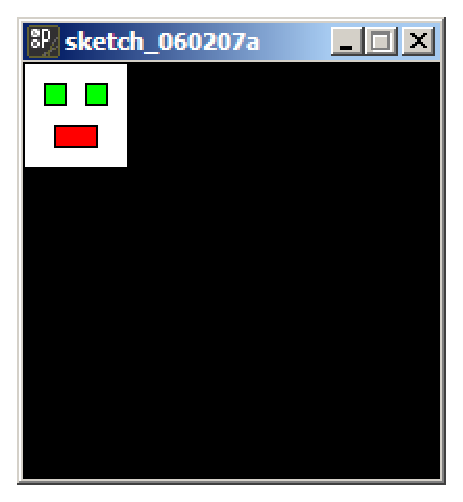
\includegraphics[width=4cm]{images/cara.eps}
\end{center}
\begin{lstlisting}
void setup() {
    size(200, 200);
}


void draw() {
    background(0);
    
    fill(255, 255, 255);     //branco
    rect(0, 0, 50, 50);      //cara
    
    fill(0, 255, 0);         //verde
    rect(10, 10, 10, 10);    //olho esquerdo
    rect(30, 10, 10, 10);    // olho direito
    
    fill(255, 0, 0);         //vermelho
    rect(15, 30, 20, 10);    // boca
}
\end{lstlisting}

Agora, em vez de apenas uma ``cara'', queremos duas:
\begin{center}
	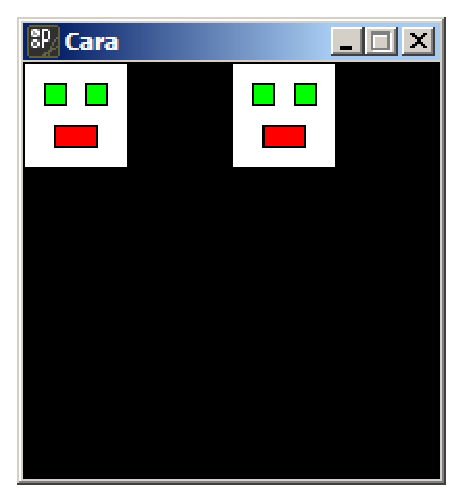
\includegraphics[width=4cm]{images/cara2.eps}
\end{center}
\begin{lstlisting}
void setup() {
    size(200, 200);
}


void draw() {
    background(0);
    
    fill(255, 255, 255);     //branco
    rect(0, 0, 50, 50);      //cara
    
    fill(0, 255, 0);         //verde
    rect(10, 10, 10, 10);    //olho esquerdo
    rect(30, 10, 10, 10);    // olho direito
    
    fill(255, 0, 0);         //vermelho
    rect(15, 30, 20, 10);    // boca

    // segunda cara
    fill(255, 255, 255);     //branco
    rect(100, 0, 50, 50);      //cara
    
    fill(0, 255, 0);         //verde
    rect(110, 10, 10, 10);    //olho esquerdo
    rect(130, 10, 10, 10);    // olho direito
    
    fill(255, 0, 0);         //vermelho
    rect(115, 30, 20, 10);    // boca    
}
\end{lstlisting}
E agora, três:
\begin{center}
	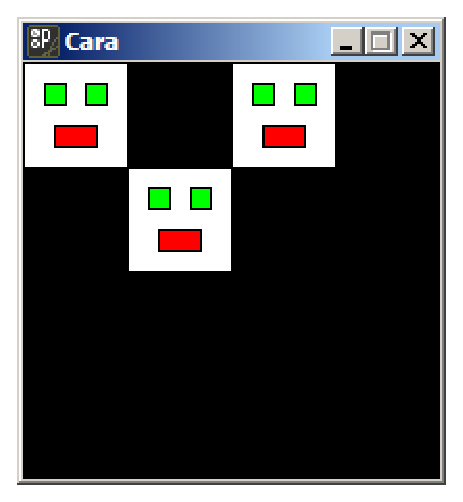
\includegraphics[width=4cm]{images/cara3.eps}
\end{center}
\begin{lstlisting}
void setup() {
    size(200, 200);
}


void draw() {
    background(0);
    
    fill(255, 255, 255);     //branco
    rect(0, 0, 50, 50);      //cara
    
    fill(0, 255, 0);         //verde
    rect(10, 10, 10, 10);    //olho esquerdo
    rect(30, 10, 10, 10);    // olho direito
    
    fill(255, 0, 0);         //vermelho
    rect(15, 30, 20, 10);    // boca
    
    // segunda cara
    fill(255, 255, 255);     //branco
    rect(100, 0, 50, 50);      //cara
    
    fill(0, 255, 0);         //verde
    rect(110, 10, 10, 10);    //olho esquerdo
    rect(130, 10, 10, 10);    // olho direito
    
    fill(255, 0, 0);         //vermelho
    rect(115, 30, 20, 10);    // boca       
    
    // terceira cara
    fill(255, 255, 255);     //branco
    rect(50, 50, 50, 50);      //cara
    
    fill(0, 255, 0);         //verde
    rect(60, 60, 10, 10);    //olho esquerdo
    rect(80, 60, 10, 10);    // olho direito
    
    fill(255, 0, 0);         //vermelho
    rect(65, 80, 20, 10);    // boca           
}

\end{lstlisting}
Se repararem, o código para desenhar as três caras é muito semelhante. Então para quê repeti-lo? A única coisa que muda é a posição onde os rectângulos são desenhados. Para isso podemos utilizar as funções. 

Uma função, ou método%
\footnote{Utilizo as palavras \emph{função} e \emph{método} com o mesmo significado.}%
, é um bloco de código com nome que pode ser executado em qualquer parte do programa. Uma função pode ser chamada%
\footnote{\emph{Chamar} ou \emph{invocar} uma função significa executar o código associado a essa função.}
várias vezes no programa, em pontos distintos.

No caso do exemplo, podemos definir duas variáveis: \texttt{x} e \texttt{y} que indicam onde a ``cara'' irá ser desenhada e criar uma função que utiliza essas variáveis para desenhar apenas uma ``cara'':
\begin{center}
	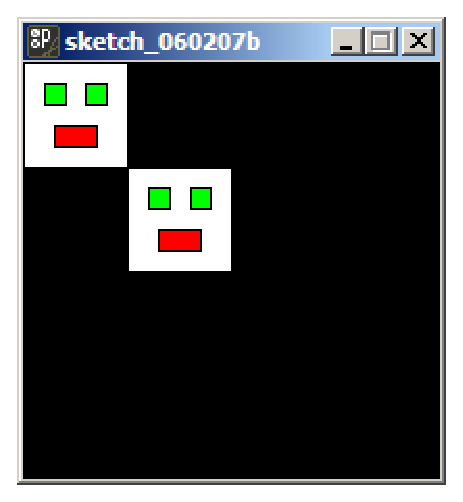
\includegraphics[width=4cm]{images/caraMetodo.eps}
\end{center}
\begin{lstlisting}
int x;
int y;

void setup() {
    size(200, 200);
}

void draw() {
    background(0);
    
    x = 0;
    y = 0;
    desenhaCara();
    
    x = 50;
    y = 50;     
    desenhaCara();  
}

void desenhaCara() {
    fill(255, 255, 255);         //branco
    rect(x, y, 50, 50);          //cara
    
    fill(0, 255, 0);             //verde
    rect(x+10, y+10, 10, 10);    //olho esquerdo
    rect(x+30, y+10, 10, 10);    // olho direito
    
    fill(255, 0, 0);             //vermelho
    rect(x+15, y+30, 20, 10);    // boca       
}
\end{lstlisting}
Neste programa, apenas escrevemos uma vez o código para desenhar a ``cara''. Tivemos de o reescrever ligeiramente de forma a utilizar as variáveis \texttt{x} e \texttt{y} como referência para a posição dos rectângulos, mas nada mais.
Assim, a única coisa que temos de fazer quando quisermos desenhar uma cara é definir a posição e invocar o método \texttt{desenhaCara()}.

Poderiamos, inclusive, utilizar um ciclo para desenhar ``caras''.


\section{Parâmetros}
No exemplo anterior, utilizámos variáveis globais para definir a posição da próxima cara a ser desenhada pela função \texttt{desenhaCara()}. No entanto, seria mais prático se pudessemos ``dizer'' ao programa: \\
-- Desenha uma cara na posição (x, y). Sem recorrer a variáveis globais.

De facto é possível. Uma das características das funções é permitir receber parâmetros que afectam a forma como a função se comporta. Os parâmetros, que não são mais do que valores (qualquer tipo de valor), são passados entre parentesis, a seguir ao nome da função. O parâmetro é identificado pela sua posição relativa, quando definimos a função. Para exemplificar, vamos redefinir a função \texttt{desenhaCara}, de modo a aceitar dois parâmetros: a posição x e a posição y da cara:
\begin{lstlisting}
void desenhaCara(int posicaoX, int posicaoY) {
    fill(255, 255, 255);         //branco
    rect(posicaoX, posicaoY, 50, 50);          //cara
    
    fill(0, 255, 0);             //verde
    rect(posicaoX+10, posicaoY+10, 10, 10);    //olho esquerdo
    rect(posicaoX+30, posicaoY+10, 10, 10);    // olho direito
    
    fill(255, 0, 0);             //vermelho
    rect(posicaoX+15, posicaoY+30, 20, 10);    // boca       
}
\end{lstlisting}
Reparem que colocamos entre parentesis, dois parâmetros: \texttt{posicaoX} e \texttt{posicaoY}. A declaração dos parâmetros é feita de forma semelhande à declaração de variáveis. Temos de indicar qual o tipo e nome da variável. Os vários parâmetros são separados por vírgulas. Dentro da função utilizamos os nomes dos parâmetros%
\footnote{Os parâmetros são, de facto, variáveis locais à função.}
 em vez de os nomes das variáveis globais.
 
Agora só nos falta saber como invocar a nova função. Vamos reescrever o método \texttt{draw()} do exemplo anterior:
\begin{lstlisting}
void draw() {
    background(0);
    
    desenhaCara(0, 0);
    
    desenhaCara(50, 50);  
}
\end{lstlisting}

Agora indicamos a posição da cara directamente na invocação da função. O primeiro valor representa a posição em X e o segundo valor representa a posição em Y. Foi esta a ordem em que definimos os parâmetros na função. 

Obviamente que os valores que passamos na invocação de uma função podem ser o resultado de uma expressão que pode conter variáveis, valores literais ou até outras funções.



\section{Valor de Retorno}

A função que utilizámos nos exemplos anteriores não podia ser utilizada numa expressão como:
\begin{lstlisting}
int x;

x = 3*5 + desenhaCara(20, 20);
\end{lstlisting}
Qual seria o resultado daquela expressão? Para isso precisamos de saber qual o valor a substituir por \texttt{desenhaCara(20, 20)}. Esse valor não existe.

O método \texttt{desenhaCara()} foi declarado como \texttt{void}%
\footnote{A \emph{keyword} \texttt{void} significa \emph{vazio}. Esta \emph{keyword} é utilizada para declarar métodos que não retornam nenhum valor.}%
.
Isto significa que o método não retorna nenhum valor e, por isso, não pode ser usado em expressões de atribuição. Apenas pode ser invocado.

No entanto, há casos em que nos interessa criar funções que fazem determinados cálculos sobre os parâmetros que lhes passamos e que devolvem o resultado desse cálculo. 

Por exemplo vamos supor que precisamos de calcular, para cada equipa do campeonato nacional, a sua pontuação actual.
Para isso precisámos de saber o número de vitórias e empates, uma vez que a pontuação é dada pela fórmula:
 \begin{equation}
pontuacao = vitorias*3 + empates
 \end{equation}
Uma vez que queremos calcular a pontuação de todas as equipas, vamos utilizar vectores para guardar a informação de todas as equipas -- um vector para guardar o número de vitórias, outro para guardar o número de empates e outro para guardar o resultado final do cálculo da pontuação. Vamos inicializar estas estruturas%
\footnote{Pontuação da Primeira Liga 2005/2006, em 13 Fevereiro de 2006. Podemos ver claramente que o Benfica será campeão! ;)}%
:
\begin{lstlisting}
int vitorias[];
int empates[];
int pontuacao[];

void setup() {
    vitorias = new int[18];
    vitorias[0] = 14; // FC Porto
    vitorias[1] = 13; // Sporting
    vitorias[2] = 13; // Benfica 
    vitorias[3] = 12; // Sp. Braga 
    vitorias[4] = 11; // Nacional
    vitorias[5] = 10; // Boavista
    vitorias[6] = 10; // V. Setúbal
    vitorias[7] = 9;  // U. Leiria
    vitorias[8] = 6;  // Marítimo
    vitorias[9] = 7;  // E. Amadora
    vitorias[10] = 6; // Rio Ave
    vitorias[11] = 7; // Académica
    vitorias[12] = 7; // Belenenses
    vitorias[13] = 7; // Paços Ferreira
    vitorias[14] = 7; // Gil Vicente
    vitorias[15] = 6; // Naval
    vitorias[16] = 4; // V. Guimarães
    vitorias[17] = 2; // Penafiel

    empates = new int[18];
    empates[0] = 6;
    empates[1] = 4;
    empates[2] = 4;
    empates[3] = 5;
    empates[4] = 6;
    empates[5] = 8;
    empates[6] = 3;
    empates[7] = 4;
    empates[8] = 9;
    empates[9] = 6;
    empates[10] = 8;
    empates[11] = 5;
    empates[12] = 4;
    empates[13] = 4;
    empates[14] = 3;
    empates[15] = 3;
    empates[16] = 5;
    empates[17] = 5;
}
\end{lstlisting}
Vamos agora calcuar a pontuação de cada equipa, à moda antiga, i.e., sem recorrer a métodos:
\begin{lstlisting}
    pontuacao = new int[18];
    pontuacao[0] = vitorias[0]*2 +empates[0];
    pontuacao[1] = vitorias[1]*2 +empates[1];
    pontuacao[2] = vitorias[2]*2 +empates[2];
    pontuacao[3] = vitorias[3]*2 +empates[3];
    pontuacao[4] = vitorias[4]*2 +empates[4];
    pontuacao[5] = vitorias[5]*2 +empates[5];                
    pontuacao[6] = vitorias[6]*2 +empates[6];
    pontuacao[7] = vitorias[7]*2 +empates[7];
    pontuacao[8] = vitorias[8]*2 +empates[8];
    pontuacao[9] = vitorias[9]*2 +empates[9];
    pontuacao[10] = vitorias[10]*2 +empates[10];
    pontuacao[11] = vitorias[11]*2 +empates[11];                        
    pontuacao[12] = vitorias[12]*2 +empates[12];                        
    pontuacao[13] = vitorias[13]*2 +empates[13];                        
    pontuacao[14] = vitorias[14]*2 +empates[14];                        
    pontuacao[15] = vitorias[15]*2 +empates[15];                        
    pontuacao[16] = vitorias[16]*2 +empates[16];                        
    pontuacao[17] = vitorias[17]*2 +empates[17]; 
\end{lstlisting}
É necessário repetir 18 vezes a expressão para calcular a pontuação! Oops, enganei-me nas contas: multipliquei por 2 em vez de por 3... tenho de corrigir 18 linhas de código:
\begin{lstlisting}
    pontuacao = new int[18];
    pontuacao[0] = vitorias[0]*3 +empates[0];
    pontuacao[1] = vitorias[1]*3 +empates[1];
    pontuacao[2] = vitorias[2]*3 +empates[2];
    pontuacao[3] = vitorias[3]*3 +empates[3];
    pontuacao[4] = vitorias[4]*3 +empates[4];
    pontuacao[5] = vitorias[5]*3 +empates[5];                
    pontuacao[6] = vitorias[6]*3 +empates[6];
    pontuacao[7] = vitorias[7]*3 +empates[7];
    pontuacao[8] = vitorias[8]*3 +empates[8];
    pontuacao[9] = vitorias[9]*3 +empates[9];
    pontuacao[10] = vitorias[10]*3 +empates[10];
    pontuacao[11] = vitorias[11]*3 +empates[11];                        
    pontuacao[12] = vitorias[12]*3 +empates[12];                        
    pontuacao[13] = vitorias[13]*3 +empates[13];                        
    pontuacao[14] = vitorias[14]*3 +empates[14];                        
    pontuacao[15] = vitorias[15]*3 +empates[15];                        
    pontuacao[16] = vitorias[16]*3 +empates[16];                        
    pontuacao[17] = vitorias[17]*3 +empates[17]; 
\end{lstlisting}
Tem de haver uma forma mais simples de fazer isto! E há: os métodos. Vamos criar um método que aceita como parâmetros o número de vitórias e o número de empates e, com base nestes parâmetros, calcula a pontuação:
\begin{lstlisting}
void calculaPontuacao(int vitoria, int empate) {
    int pontos = vitoria*3 + empate;
}
\end{lstlisting}
A única coisa que este método faz, para já, é implementar a expressão da pontuação. Para podermos tirar partido deste método temos de arranjar forma de obter o resultado do cálculo. Para isso temos de redefinir o método, de forma a indicar o tipo de valor que o método devolve. Depois basta utilizar a \emph{keyword} \texttt{return} no final do método para devolver o resultado:
\begin{lstlisting}
int calculaPontuacao(int vitoria, int empate) {
    int pontos = vitoria*3 + empate;
    
    return pontos;
}
\end{lstlisting}
Agora podemos reescrever o nosso programa:
\begin{lstlisting}
    pontuacao = new int[18];
    pontuacao[0] = calculaPontuacao(vitorias[0], empates[0]);
    pontuacao[1] = calculaPontuacao(vitorias[1], empates[1]);
    pontuacao[2] = calculaPontuacao(vitorias[2], empates[2]);
    pontuacao[3] = calculaPontuacao(vitorias[3], empates[3]);
    pontuacao[4] = calculaPontuacao(vitorias[4], empates[4]);
    pontuacao[5] = calculaPontuacao(vitorias[5], empates[5]);                
    pontuacao[6] = calculaPontuacao(vitorias[6], empates[6]);
    pontuacao[7] = calculaPontuacao(vitorias[7], empates[7]);
    pontuacao[8] = calculaPontuacao(vitorias[8], empates[8]);
    pontuacao[9] = calculaPontuacao(vitorias[9], empates[9]);
    pontuacao[10] = calculaPontuacao(vitorias[10], empates[10]);
    pontuacao[11] = calculaPontuacao(vitorias[11], empates[11]);                        
    pontuacao[12] = calculaPontuacao(vitorias[12], empates[12]);                        
    pontuacao[13] = calculaPontuacao(vitorias[13], empates[13]);                        
    pontuacao[14] = calculaPontuacao(vitorias[14], empates[14]);                        
    pontuacao[15] = calculaPontuacao(vitorias[15], empates[15]);                        
    pontuacao[16] = calculaPontuacao(vitorias[16], empates[16]);                       
    pontuacao[17] = calculaPontuacao(vitorias[17], empates[17]);
\end{lstlisting}
Agora, se por acaso nos tivessemos enganado na expressão da pontuação, apenas tinhamos de alterar uma linha de código!
No entanto, ainda temos muitas linhas de código iguais... vamos resolver isso com um ciclo. O código final do nosso programa seria:
\begin{lstlisting}
int vitorias[];
int empates[];
int pontuacao[];

void setup() {
    int i;
    
    vitorias = new int[18];
    vitorias[0] = 14; // FC Porto
    vitorias[1] = 13; // Sporting
    vitorias[2] = 13; // Benfica 
    vitorias[3] = 12; // Sp. Braga 
    vitorias[4] = 11; // Nacional
    vitorias[5] = 10; // Boavista
    vitorias[6] = 10; // V. Setúbal
    vitorias[7] = 9;  // U. Leiria
    vitorias[8] = 6;  // Marítimo
    vitorias[9] = 7;  // E. Amadora
    vitorias[10] = 6; // Rio Ave
    vitorias[11] = 7; // Académica
    vitorias[12] = 7; // Belenenses
    vitorias[13] = 7; // Paços Ferreira
    vitorias[14] = 7; // Gil Vicente
    vitorias[15] = 6; // Naval
    vitorias[16] = 4; // V. Guimarães
    vitorias[17] = 2; // Penafiel

    empates = new int[18];
    empates[0] = 6;
    empates[1] = 4;
    empates[2] = 4;
    empates[3] = 5;
    empates[4] = 6;
    empates[5] = 8;
    empates[6] = 3;
    empates[7] = 4;
    empates[8] = 9;
    empates[9] = 6;
    empates[10] = 8;
    empates[11] = 5;
    empates[12] = 4;
    empates[13] = 4;
    empates[14] = 3;
    empates[15] = 3;
    empates[16] = 5;
    empates[17] = 5;
    
    pontuacao = new int[18];
    for (i = 0; i < 18; i = i + 1) {
        pontuacao[i] = calculaPontuacao(vitorias[i], empates[i]);
    }

}

int calculaPontuacao(int vitoria, int empate) {
    int pontos = vitoria*3 + empate;
    
    return pontos;
}
\end{lstlisting}

O método \texttt{calculaPontuacao()} é diferente dos métodos que criamos anteriormente porque \emph{retorna} um valor. 
Por isso alteramos a declaração do método: em vez de \texttt{void} usámos \texttt{int}, para indicar que o nosso método retorna um valor do tipo \texttt{int}. 
No código do nosso método, a \emph{keyword} \texttt{return} é utilizada para devolver o valor ao código que invocou o nosso método. Quando retornamos um valor, terminamos também a execução do código do nosso método, ou seja, código a seguir ao \texttt{return} nunca é executado. O \texttt{return} pode ser utilizado em qualquer parte do método. Podemos, por exemplo, colocá-lo dentro de um \texttt{if} de forma a retornar valores diferentes consoante a condição...

Os métodos que retornam valores podem ser utilizados em expressões de atribuição. Foi exactamente isso que fizemos no nosso exemplo:
\begin{lstlisting}
    pontuacao[0] = calculaPontuacao(vitorias[0], empates[0]);
\end{lstlisting}
Quando o programa chega a esta linha de código, irá executar o nosso método com os valores dos parâmetros:
\begin{lstlisting}
    pontuacao[0] = calculaPontuacao(14, 6);
\end{lstlisting}
O código do método executa e devolve o valor $14 \times 3+6$ (48):
\begin{lstlisting}
    pontuacao[0] = 48;
\end{lstlisting}

\section{(Quase) Tudo São Métodos}
Grande parte dos programas que escrevemos utilizam métodos definidos pela própria linguagem. Temos vindo a utilizar até aqui métodos como \texttt{rect()}, para desenhar um rectângulo; \texttt{background()} para limpar o fundo do ecrã com uma determinada cor; \texttt{fill()} para mudar a cor de preenchimento do próximo objecto desenhado; etc.
Estes métodos são em tudo semelhantes aos métodos que nós próprios definimos no nosso programa. A única diferença, é que estes foram definidos pela linguagem.

\subsection{Call Me Back... (Callbacks)}
Como vimos, podemos definir os nossos próprios métodos de forma a estruturar melhor o código do nosso programa.
Vimos também, que o Processing possui um conjunto de métodos próprios que podemos utilizar.

No fundo, o que distingue as linguagens de programação é a sua sintaxe e o conjunto de métodos que estão disponíveis ao programador.

Existem alguns métodos que, apesar de sermos nós (programadores) a implementar%
\footnote{\emph{Implementar um método}, é declará-lo e escrever o código que executa dentro desse método.}%
, não somos nós que os invocamos. Estes métodos são métodos pré-definidos pelo Processing, mas que o programador deve re-implementar para tirar partido deles. Por exemplo, o método \texttt{draw()}. Apesar de termos de o declarar e implementar, nunca o invocamos. 

Estes métodos são chamados métodos de \emph{callback}%
\footnote{\emph{Callback}, porque estes métodos são invocados pela própria linguagem em resposta a um evento externo. Ou seja, são \emph{chamados de volta} pela linguagem.}%
.
 
Existem mais métodos de \emph{callback} para além do \texttt{draw()}:
\begin{itemize}
\item \texttt{setup()} -- invocado pelo Processing antes de iniciar o nosso programa. Este método serve para inicializarmos as nossas variáveis. Devemos colocar aqui o código que queremos que execute apenas uma vez, no início do programa.

\item \texttt{draw()} -- invocado periodicamente pelo Processing para actualizar o estado do programa. Neste método devemos colocar o código para desenhar o nosso programa. A frequência com que este método é invocado pelo Processing pode ser controlado.

\item \texttt{keyPressed()} -- invocado pelo Processing quando o utilizador carrega numa tecla do teclado. 

\item \texttt{keyReleased()} -- invocado pelo Processing quando o utilizador larga uma tecla do teclado. 

\item \texttt{mousePressed()} -- invocado pelo Processing quando o utilizador clica num botão do rato.

\item \texttt{mouseMoved()} -- invocado pelo Processing quando o utilizador arrasta o rato.

\item \texttt{mouseDragged()} -- invocado pelo Processing quando o utilizador arrasta o rato mantendo um botão pressionado.

\item \texttt{mouseReleased()} --	invocado pelo Processing quando o utilizador larga um botão do rato.
\end{itemize}

\section{Métodos e Variáveis}
Um programa pode ser visto como um conjunto de caixas espelhadas: se estivermos dentro da caixa conseguimos ver o que se passa cá fora, mas quem está de fora não consegue ver o interior da caixa.
Uma caixa grande representa o programa principal e caixas mais pequenas, dentro da caixa grande, representam os métodos. É útil pensar nestes termos quando queremos entender a visibilidade das variáveis. Uma variável local ao método está ``dentro da caixa pequena'' que representa esse método. Assim, a ``caixa grande'' -- o programa principal -- não consegue aceder às variáveis declaradas no método, mas o método consegue aceder às variáveis do programa principal. De igual modo, um método não consegue ``ver'' as variáveis locais a outro método. A Figura[x] ilustra esta metáfora.
\begin{figure}
	\centering
		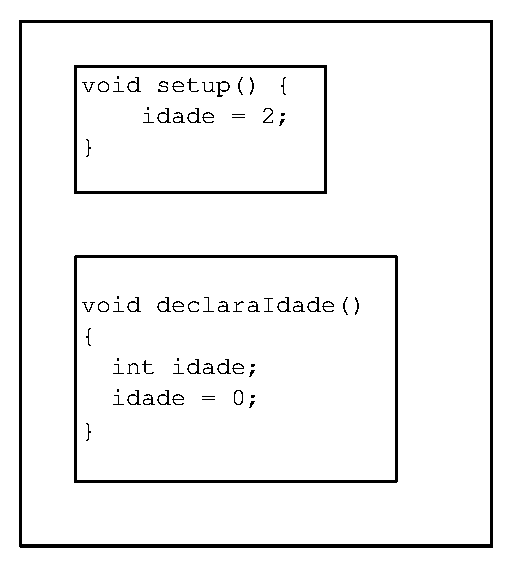
\includegraphics{images/cap6-visibilidade-1.eps}
	\caption{Visibilidade de variáveis locais}
	\label{fig:cap6-visibilidade-1}
\end{figure}

\section{Exercícios}
\begin{enumerate}
\item 
Reescreva um dos programas que criou até agora de forma a utilizar métodos.

\item 
Crie um programa que desenha várias mensagens na janela gráfica.

\item
Adapte o exemplo das caras, de modo a utilizar um \texttt{for} para desenhar 100 caras em posições diferentes no ecrã.
\end{enumerate}

\chapter{Com Classe! (Classes e Objectos)}

\section{Objectos e Classes}
Já vimos nos primeiros capítulos que as variáveis guardam um determinado tipo de dados e vimos também já alguns tipos de dados primitivos ou simples, como o \texttt{int}, \texttt{boolean} e \texttt{float}.

No entanto, em Processing, existe um outro tipo de dados que pode ser definido pelo programador. Estes tipos são representados por \emph{objectos}. Um objecto é uma estrutura de dados e funcionalidade. Ou seja, não serve apenas para armazenar dados, mas também pode ter associado métodos. Desta forma podemos agrupar dados e métodos que operam sobre esses dados, de forma mais estruturada.

A definição destes tipos de dados é feita através daquilo que se chama, em programação, uma \emph{classe}. 
Apenas para dar um exemplo simples de uma classe, vejamos o código seguinte:
\begin{lstlisting}
public class Pessoa {
    String nome;
    int anoNascimento;
    int altura;
    
    public Pessoa(String nomePessoa, int anoNasc, int alturaPessoa) {
        nome = nomePessoa;
        anoNascimento = anoNasc;
        altura = alturaPessoa;
    }
    
    public int calculaIdade() {
        return year()-anoNascimento;
    }   
}
\end{lstlisting}


O exemplo define uma classe que representa uma pessoa. Neste exemplo, usamos apenas o nome, o ano de nascimento e a altura para representar uma pessoa. Para além dos dados, podemos ver que a classe define também métodos que operam sobre esses dados. O método \texttt{calculaIdade()} calcula a idade da pessoa tendo em conta o ano de nascimento (\texttt{anoNascimento}) e o ano em que estamos (\texttt{year()}). O método \texttt{Pessoa()} é um método especial, designado por \emph{construtor} da classe.

\subsection{Construtores}
Um construtor é um método especial que serve para construir o objecto da classe correspondente. Como podemos ver no exemplo anterior, o construtor é utilizado para inicializar as variáveis que representam a pessoa.
Para construirmos um objecto da classe que criámos atrás, teriamos de escrever algo como:
\begin{lstlisting}
Pessoa joao;

joao = new Pessoa("João", 1980, 174);
\end{lstlisting}
Primeiro temos de declarar uma variável do tipo \texttt{Pessoa}. Depois temos de criar o objecto \texttt{Pessoa} correspondente e reservar espaço na memória do computador para guardar todos os dados associados a uma \texttt{Pessoa}. Isso é feito na linha seguinte, utilizando a \emph{keyword} \texttt{new} (tal como nos vectores) e invocando o construtor com os parâmetros necessários.

Depois de termos o nosso objecto criado, podemos invocar o método que calcula a idade do \texttt{joao}:
\begin{lstlisting}
print(joao.calculaIdade());
\end{lstlisting}

Para invocarmos um método de um objecto temos de utilizar a notação \emph{ponto}. Ou seja, escrevemos o nome do objecto seguido de um ``.'' (ponto final), seguido no nome e parâmetros do método que estamos a invocar.
Obviamente, apenas podemos invocar métodos que tenham sido definidos na classe do objecto (no nosso exemplo apenas definimos um -- \texttt{calculaIdade()}).


\subsection{Texto (\texttt{String})}
Existe um tipo de dados muito utilizado e que ainda não abordamos: a \texttt{String}. Uma string é um pedaço de texto. Em Processing, uma string é representada pela classe \texttt{String}%
\footnote{Noutras linguagens de programação, uma string pode ser representada de forma diferente.}
.

Por exemplo, se o nosso programa necessitar de armazenar o nome do utilizador, teriamos de declarar uma variável do tipo
\texttt{String}:
\begin{lstlisting}
String nomeUtilizador;
\end{lstlisting}

Uma vez que uma \texttt{String} é uma classe, para criarmos um objecto deste tipo temos de invocar o construtor:
\begin{lstlisting}
nomeUtilizador = new String("jorge");

print(nomeUtilizador);
\end{lstlisting}
As strings são representadas por texto entre aspas.

De resto, as classes comportam-se como um tipo de dados simples, pelo que podemos, por exemplo, criar um vector de strings:
\begin{lstlisting}
String nomes[];

nomes = new String[10];

nomes[0] = new String("Joao");
nomes[1] = new String("Jorge");
...
nomes[9] = new String("André");
\end{lstlisting}
Tenham em atenção que, neste exemplo, demos dois usos diferentes à \emph{keyword} \texttt{new}: primeiro para reservar espaço de memória para o vector e depois para reservar espaço de memória para cada elemento desse vector (porque cada elemento é uma string).

\chapter{Comentário Final (Documentação)}

Um programa não é apenas formado pelo conjunto de instruções da linguagem de programação. Se assim fosse, a maioria dos programas seria ininteligíveis para nós. Atentem no programa do Exemplo [x]. O que faz esse programa? Como o faz? Como o modificamos para o adaptar a outra situação? Torna-se difícil (embora não impossível) responder a estas perguntas, porque o programa não está documentado. Agora observem o Exemplo [xpto].

\section{Comentários}
Os comentários são pedaços de texto que não afectam a execução do programa e que 
servem para documentar o código, explicando o funcionamento do programa.

Os comentários devem ser usados para explicar secções de código cujo significado não
seja óbvio\footnote{O significado é óbvio ou não dependendo do contexto.}.

De forma a que o compilador possa distinguir entre texto de comentários e texto
do programa é necessário que os comentários sejam identificados por símbolos especiais.
Existem dois tipos de comentários:
\begin{description}
\item[Linha] Os comentários de linha são identificados pelos caracteres ``\texttt{//}''. 
Todo o texto seguinte na linha é considerado comentário e, portanto, ignorado. Exemplo:
\begin{lstlisting}
int altura[100]; // a altura de 100 pessoas em centímetros
\end{lstlisting}
\item[Bloco] Os comentários de bloco servem para definir um comentário que se prolonga por
várias linhas. Os comentários de bloco são delimitados por duas sequências de caracteres:
``\texttt{/*}'' e ``\texttt{*/}''. Estes comentários permitem-nos dar uma explicação mais
longa sobre o código. Exemplo:
\begin{lstlisting}
/* Determinar a altura máxima e mínima do grupo de pessoas.
   Precisamos de variáveis temporárias para armazenar as 
   alturas miníma e máxima enquanto estamos a percorrer o 
   vector. */
   int minimo = 0, maximo = 10000;
   int i;
   for (i = 0; i < 100; i = i + 1) {
       if (altura[i] < minimo) {           
           minimo = altura[i];
       } else if (altura[i] > maximo) {
           maximo = altura[i];
       }
   }
   print("Altura máxima: " + maximo);
   print("Altura miníma: " + minimo);
\end{lstlisting}
\end{description}

A utilização de um tipo de comentário ou outro é, maioritariamente, uma questão de estilo. 
Podemos utilizar indiferencialmente um ou outro. Os exemplos anteriores poderiam ter sido escritos como:
\begin{lstlisting}
inteiro altura[100]; /* A altura de 100 pessoas em centímetros */

// Determinar a altura máxima e mínima do grupo de pessoas.
// Precisamos de variáveis temporárias para armazenar as 
// alturas miníma e máxima enquanto estamos a percorrer o 
// vector.
   int minimo = 0, maximo = 10000;
   int i;
   for (i = 0; i < 100; i = i + 1) {
       if (altura[i] < minimo) {           
           minimo = altura[i];
       } else if (altura[i] > maximo) {
           maximo = altura[i];
       }
   }
   print("Altura máxima: " + maximo);
   print("Altura miníma: " + minimo);
\end{lstlisting}


\section{Exercícios}
\begin{enumerate}
\item 
Documente, se ainda não o fez, os últimos dois programas que fez.	
\end{enumerate}

\chapter{Eu Cá, Tu Lá... (Interacção)} \label{cap:interaccao}
A maioria dos programas que construímos necessitam que o utilizador
interaja com o computador. Por exemplo, se quisermos que o utilizador escolha uma entre várias opções, se pretendermos obter um texto, etc.

Existem várias formas de obter dados do utilizador. Para além do teclado e do rato, é possível utilizar sensores, camâras \emph{web}, etc. Este capítulo, no entanto, dedica-se apenas à interacção através do teclado e do rato do computador.

\section{O Rato} 
A informação que podemos obter do rato do computador resume-se à sua localização espacial (a posição (x, y) do ponteiro do rato) e o estado dos botões.

O ponteiro do rato é representado internamente, no computador, como um ponto num sistema de coordenadas bidimensional (um ponto com coordenadas (x, y)). O sistema de coordenadas tem origem (0, 0), no canto superior esquerdo da janela do Processing. A Figura~\ref{fig:coordinatesrato} exemplifica isto.
\begin{figure}
	\centering
		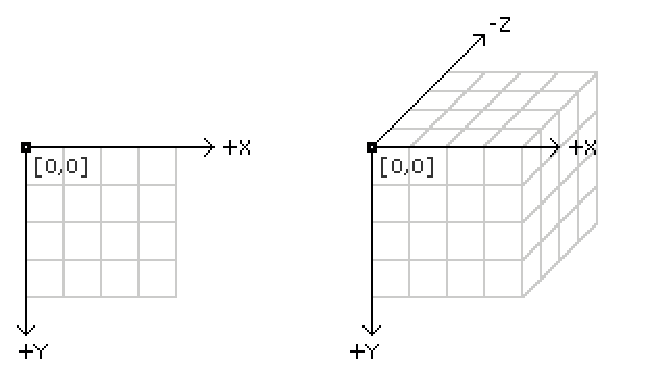
\includegraphics{images/coordinates.eps}
	\label{fig:coordinatesrato}
	\caption{O rato no sistema de coordenadas}
\end{figure}

\subsection{Posição}
A posição (x, y) do ponteiro do rato é actualizada e mantida em variáveis especiais do Processing. Estas variáveis são \texttt{mouseX} e \texttt{mouseY} (do tipo \texttt{int}) e são actualizadas constantemente pelo Processing. 

O programa seguinte (Exemplo~\ref{exe:interaccao_rato_xy}) exemplifica o uso destas variáveis.
\lstinputlisting[caption=Posição do Rato \\~% 
\texttt{[interaccao\_rato\_xy]}, label=exe:interaccao_rato_xy,%
firstline=10]{Interaccao//interaccao_rato_xy//interaccao_rato_xy.pde}

Podemos verificar que estas variáveis podem ser utilizadas como quaisquer outras variáveis, pelo que podemos passá-las como parâmetros de métodos, usá-las em expressões matemáticas, etc. 

\subsection{Botões}
O estado dos botões do rato pode ser obtido de duas formas. Podemos ``perguntar'' se um botão foi pressionado, ou podemos pedir ao Processing que nos informe sempre que um botão for pressionado.

Para a primeira forma, utilizamos a variável booleana \texttt{mousePressed} que indica se um botão está pressionado (a variável é \texttt{true} se um botão estiver pressionado e \texttt{false} se não estiver nenhum botão pressionado). Se a variável for \texttt{true}, então podemos utilizar a variável \texttt{mouseButton} para determinar qual o botão pressionado (o botão do lado esquerdo, do meio, ou da direita).

\lstinputlisting[caption=Botões do Rato Síncronos, label=exe:interaccao_rato_botoes_sincrono,%
firstline=10]{Interaccao//interaccao_rato_botoes_sincrono//interaccao_rato_botoes_sincrono.pde}

Esta forma de obter o estado dos botões é feita de forma síncrona, ou seja, o programa lê o estado dos botões do rato num ponto específico do programa. Se, quando o programa chegar ao ponto em que verifica o estado dos botões, nenhum botão estiver pressionado então não é detectado nenhum botão pressionado. Se o utilizador pressionar e largar um botão do rato enquanto o programa está a desenhar o rectângulo:
\lstinputlisting[nolol= true, firstline=26, lastline=26]%
{Interaccao//interaccao_rato_botoes_sincrono//interaccao_rato_botoes_sincrono.pde}
O programa não irá detectar este acontecimento, porque, quando chegar à linha de código que faz a verificação, o utilizador já largou o botão. Isto significa que se podem ``perder'' eventos do rato.

Para isto não acontecer, temos de obter o estado dos botões de forma assíncrona, ou seja, deixamos o Processing informar o programa sempre que um botão for pressionado. Desta forma, seja qual for o ponto em que o nosso programa estiver, os eventos são sempre detectados.
Para usarmos esta forma de obter o estado do rato permite-nos obter não só o estado dos botões mas também outros eventos do rato. Para isso utilizamos os métodos de \emph{callback} já descritos no Capítulo~\ref{cap:metodos}:

\begin{itemize}
\item \texttt{mousePressed()} -- invocado pelo Processing quando o utilizador clica num botão do rato.

\item \texttt{mouseMoved()} -- invocado pelo Processing quando o utilizador arrasta o rato.

\item \texttt{mouseDragged()} -- invocado pelo Processing quando o utilizador arrasta o rato mantendo um botão pressionado.

\item \texttt{mouseReleased()} --	invocado pelo Processing quando o utilizador larga um botão do rato.
\end{itemize}

O programa seguinte mostra como adaptar o Exemplo~\ref{exe:interaccao_rato_botoes_sincrono} para utilizar a nova forma de obter o estado dos botões.

\lstinputlisting[caption=Botões do Rato Assíncronos\\ \texttt{[interaccao\_rato\_botoes\_assincrono]}, label=exe:interaccao_rato_botoes_assincrono, firstline=10]{Interaccao//interaccao_rato_botoes_assincrono//interaccao_rato_botoes_assincrono.pde}


\section{O Teclado}
A obtenção do estado das teclas do teclado é feita de forma muito semelhante à utilizada para o rato.
Basicamente, temos os dois métodos descritos anteriormente: de forma síncrona e de forma assíncrona. 

A variável booleana \texttt{keyPressed} indica, à semelhança da variável \texttt{mousePressed} para o rato, se alguma tecla foi pressionada. A variável \texttt{key} contém o carácter associado à tecla pressionada. Para as teclas especiais, como as teclas direccionais, podemos utilizar a variável \texttt{keyCode} para verificar qual a tecla pressionada. O Exemplo~\ref{exe:interaccao_teclado_sincrono} mostra como ler as teclas pressionadas e o Exemplo~\ref{exe:interaccao_teclado_teclas_especiais} mostra como ler as teclas especiais.

\lstinputlisting[caption=Teclado \\ \texttt{[interaccao\_teclado\_sincrono]}, label=exe:interaccao_teclado_sincrono, firstline=10]{Interaccao//interaccao_teclado_sincrono//interaccao_teclado_sincrono.pde}


\lstinputlisting[caption=Teclado: Teclas Especiais \\ \texttt{[interaccao\_teclado\_teclas\_especiais]}, label=exe:interaccao_teclado_teclas_especiais, firstline=10]{Interaccao//interaccao_teclado_teclas_especiais//interaccao_teclado_teclas_especiais.pde}

Tal como no caso do rato, esta forma de ler o estado das teclas pode falhar se o utilizador pressionar e libertar a tecla antes de o programa chegar à instrução que lê o estado das teclas.

No entanto, se utilizarmos os métodos de \emph{callback}, garantimos que o programa recebe sempre os eventos do teclado.

Para o teclado, temos os métodos:
\begin{itemize}
\item \texttt{keyPressed()} -- invocado pelo Processing quando o utilizador carrega numa tecla do teclado. 

\item \texttt{keyReleased()} -- invocado pelo Processing quando o utilizador larga uma tecla do teclado. 
\end{itemize}

O exemplo seguinte mostra como utilizar estes métodos:
\lstinputlisting[caption=Teclado Assíncrono \\ \texttt{[interaccao\_teclado\_assincrono]}, label=exe:interaccao_teclado_assincrono, firstline=10]{Interaccao//interaccao_teclado_assincrono//interaccao_teclado_assincrono.pde}


%%----------------------------------------------------------------------------------------
%	CHAPTER 2
%----------------------------------------------------------------------------------------
\chapterimage{band1.png}

\chapter{Discovering what to do...}

\section{First ideas}\index{First ideas}
So, now here you have your first astronomy picture, \footnote{For example purposes the image selected is a picture of M83 through a Wide H-alpha and [N II] filter. } what do you see?, it is a monochrome image, with different levels of brightness, slightly big (8500 x 5000), it looks like a lot of stars making a spiral.
\begin{figure}[h]
    \centering
    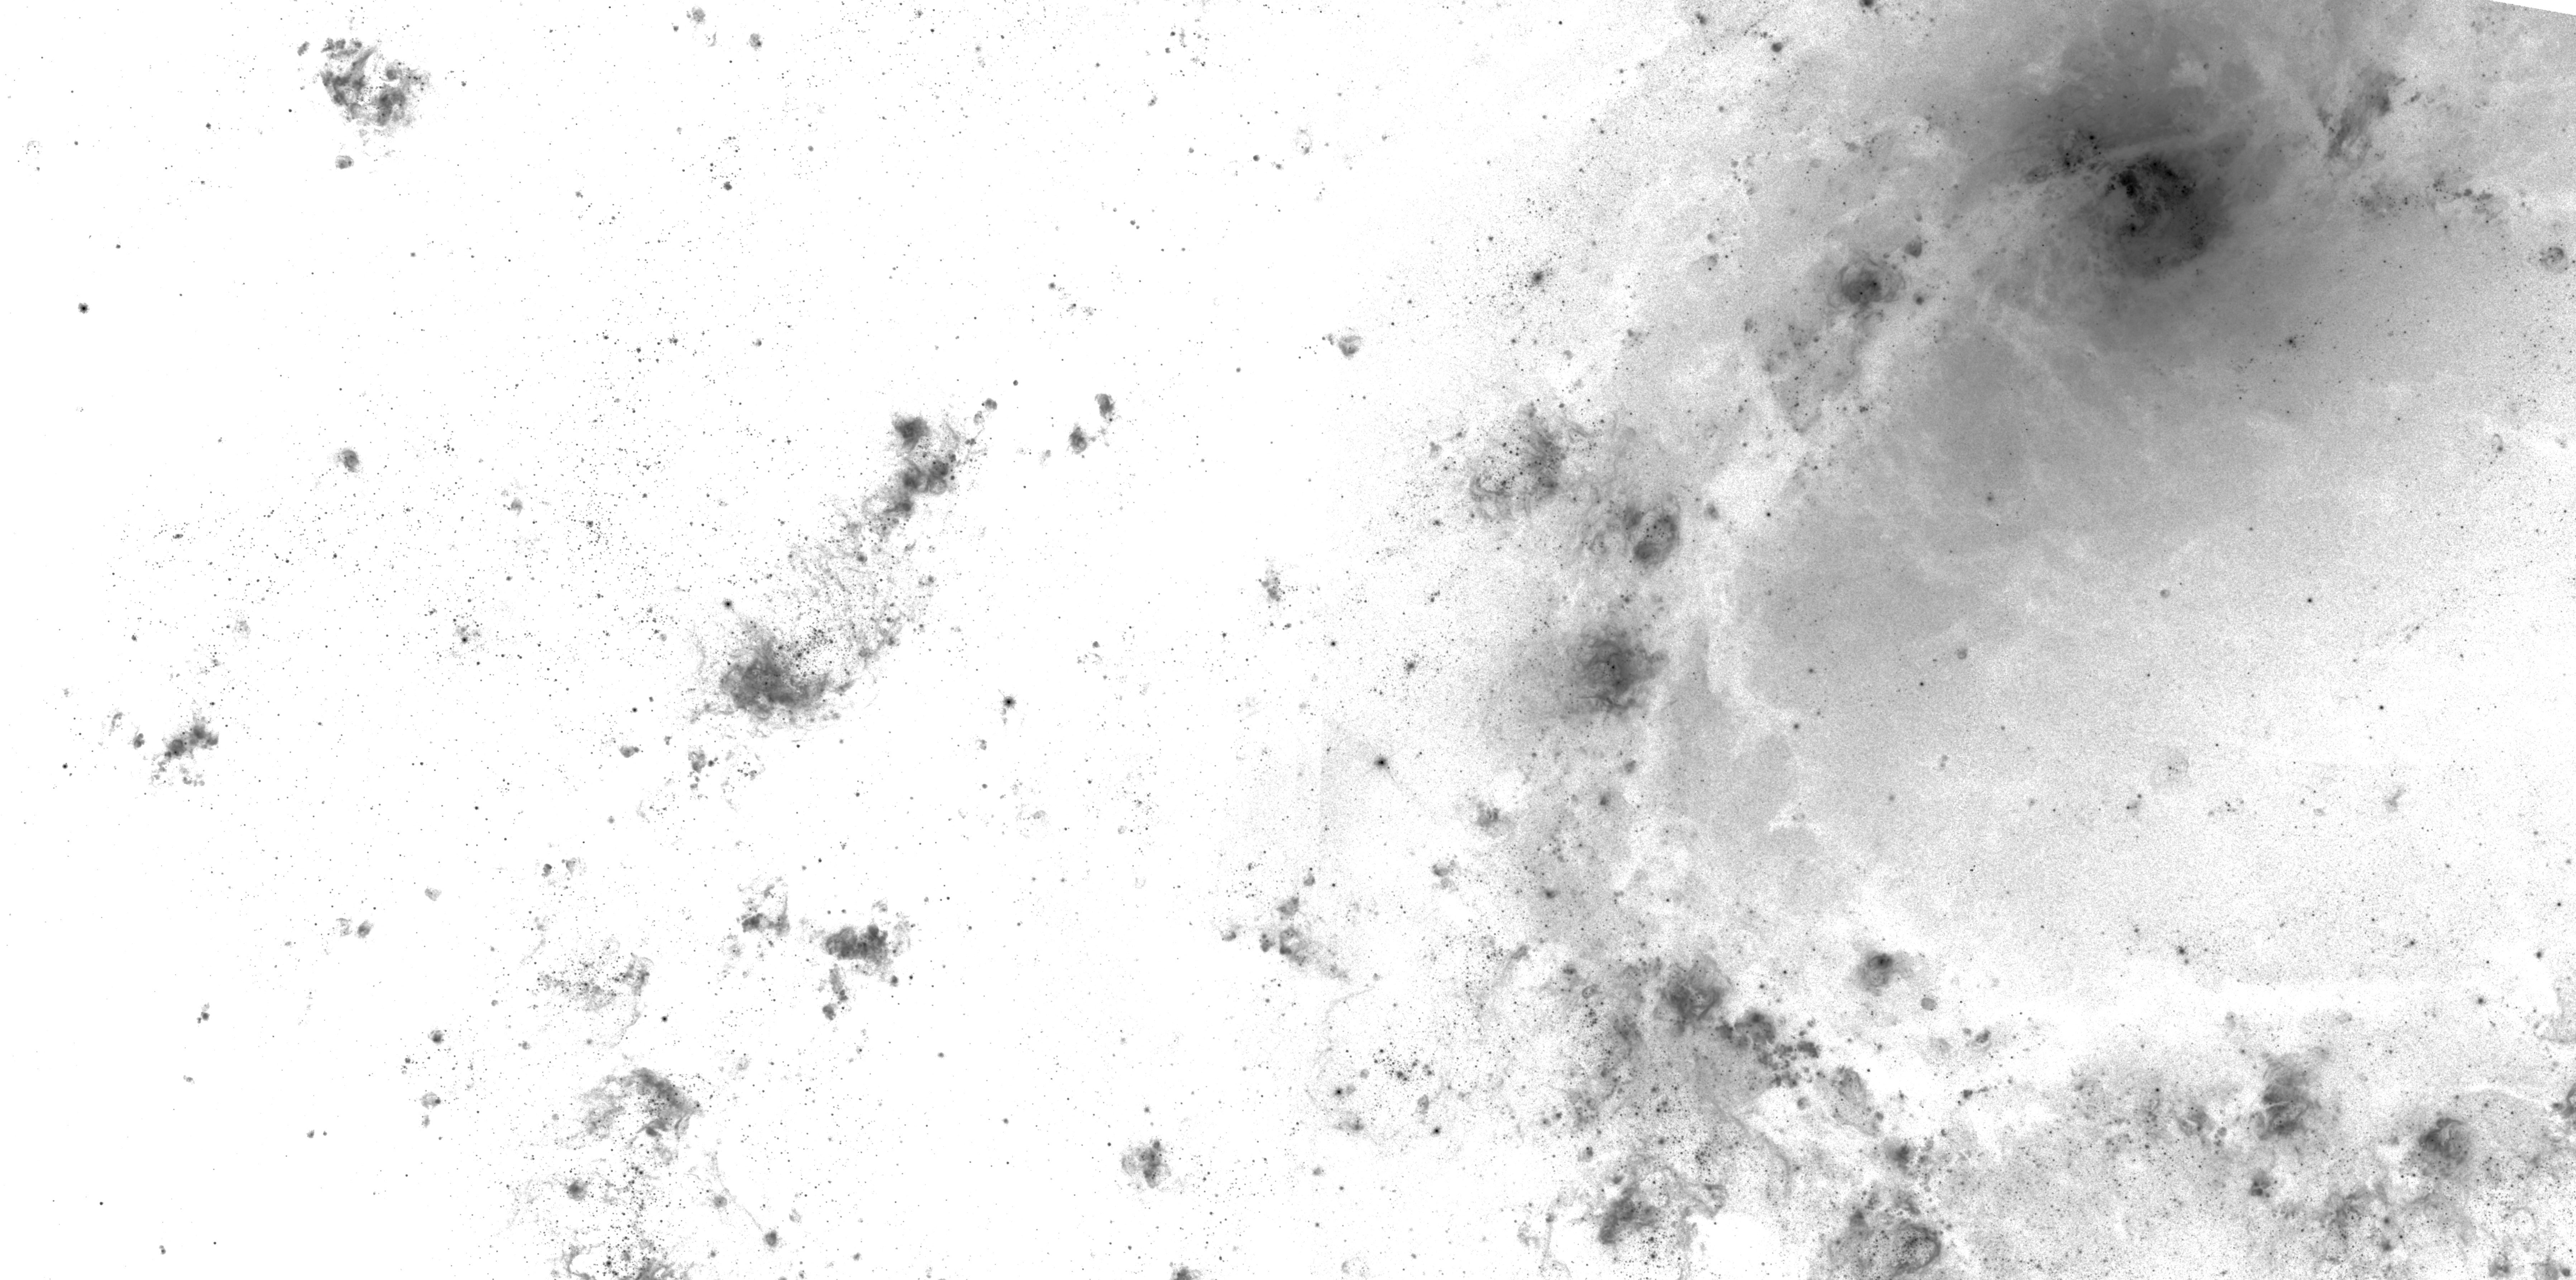
\includegraphics[width=0.77\textwidth]{ha-gray-conv-crp.jpg}
    \caption{Picuture of the M83 galaxy, image taken from the WFC3 ERS M83 Data Products, http://archive.stsci.edu/prepds/wfc3ers/m83datalist.html}
    \label{fig:awesome_image}
\end{figure}

How can we learn something about this image, quantize, get useful information? In the next subsections I will explain the first ideas.

\subsection{Superpixel segmentation}
The main concept of this is to cut an image into bigger neighborhood sections, so from an image that has $425x10^5$ pixels we can get maybe less than 500 superpixels, and then analyse separately those little sections and identify what kind of intersellar objects are they, look at image \ref{fig:super} it is a self-explanatory example of how a superpixel algorithm works.
\begin{figure}[h]
    \centering
    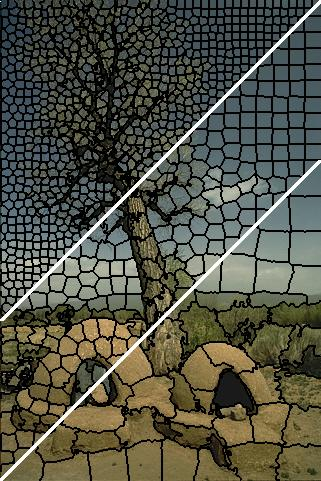
\includegraphics[width=0.37\textwidth]{combo.jpg}
    \caption{Example of a superpixel algorithm}
    \label{fig:super}
\end{figure}
There are many ways to do this and they vary according to color dimensions, methods and number of required superpixels and whether the algorithm is able to find borders and make pixel clasifications.

\begin{remark}
	You can find some example test I tested with Matlab and with Python in this webapage: \url{https://github.com/LaurethTeX/Clustering/blob/master/Methods.md}, also there is a huge amount of information on th internet about this but here are two pages you might find useful:
    \begin{itemize}
    	\item Superpixel: Empirical Studies and Applications \\ \url{http://ttic.uchicago.edu/~xren/research/superpixel/}
        \item Segmentation Algorithms in scikits-image \\ \url{http://peekaboo-vision.blogspot.ca/2012/09/segmentation-algorithms-in-scikits-image.html}
    \end{itemize}
    Also there is one article (from IEEE) I found about and might interest you, it's pure computer science,
    \begin{itemize}
    	\item Normalized Cuts and Image Segmentation \\ \url{http://www.cs.berkeley.edu/~malik/papers/SM-ncut.pdf}
    \end{itemize}
\end{remark}

\subsection{PCA}

Welcome to Astronomy where you will find more acronyms than words to mention something on articles, lots of fun!, well in this case PCA stands for Principal Component Analysis, the objective of this method is to reduce dimnensionality, tranform the data to another space where is can be manipulated and reduced, there are multiple examples of work that has been done in astronomy applying this technique.

Therefor, the idea of applying this method is that if we have multiple-wavelenght images of the same target and transform them to PCA space then we will have less dimensionality and it will be easier to process all the data and fins valuable information.\footnote{Before I forget to mention, later I discovered that PCA is not comonly used for datamining preprocessing because it is hard to interpret the information in the output result. Imagine clusters of data on PCA space, how do you make sense to that?}

\begin{figure}[h]
    \centering
    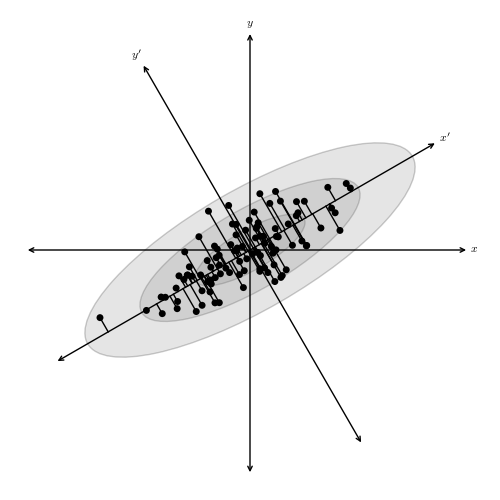
\includegraphics[width=0.37\textwidth]{fig_PCA.png}
    \caption{A distribution of points drawn from a bivariate Gaussian and centered on the origin of $x$ and $y$. PCA defines a rotation such that the new axes ($x’$ and $y’$) are aligned along the directions of maximal variance (the principal components) with zero covariance. This is equivalent to minimizing the square of the perpendicular distances between the points and the principal components}
    \label{fig:pca}
\end{figure}

\begin{remark}
	An example article, where they explain how to apply PCA on multi-wavelenght images and also mentions the pros and cons of using it.
    \begin{itemize}
    	\item Preserving Structure in Multi-wavelength Images of Extended Objects\\ \url{http://arxiv.org/abs/1101.1679v1}
    \end{itemize}
    There's a whole section that talks about this subject with a machine learning approach as a preprocessing step in this nice book,
    \begin{itemize}
    	\item Ivezi{\'c}, \v Z. and Connolly, A.J.
         and Vanderplas, J.T. and Gray, A., \textit{Statistics, Data Mining and Machine Learning in Astronomy}, Princeton University Press, Princeton, NJ, 2014.
    \end{itemize}
\end{remark}

\section{Hypothesis}\index{Hypothesis}
Our data looks like the images on Fig.\ref{fig:cubes}, and it cointains data from let's say a determined galaxy at different wavelengths, if we assume that the galaxy contains various regions that relate to interstellar objects that can tell, how stars are formed, where, how stars die, where was a star, and other mysteries, I guess we can assume that those certain regions can be identified because they share similar characteristics, the ideas is to find how a galaxy is made from, its contents, apply the concept of the superpixel idea in 3D superpixels. 
\begin{figure}[h]
	\centering
    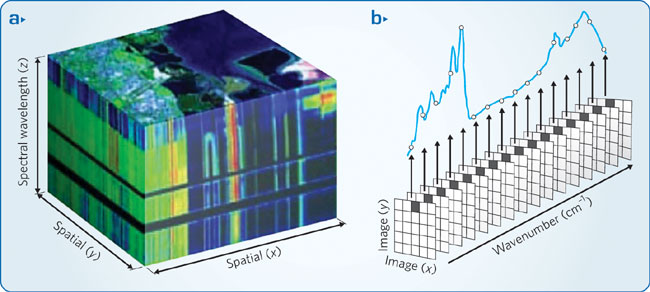
\includegraphics[width=0.57\textwidth]{nphoton.jpg}\hspace{1cm}
    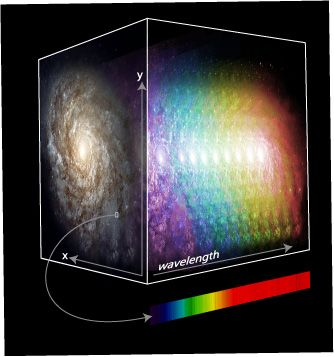
\includegraphics[width=0.27\textwidth]{data.jpg}
    \caption{Illustrations of how a datacube looks like.}
    \label{fig:cubes}
\end{figure}

Take the time to think about this, how the data looks like in 3D, how a star looks like in the datacube, imagine it, this is where ideas of how to tackle this problem come from.
\begin{figure}
	\centering
    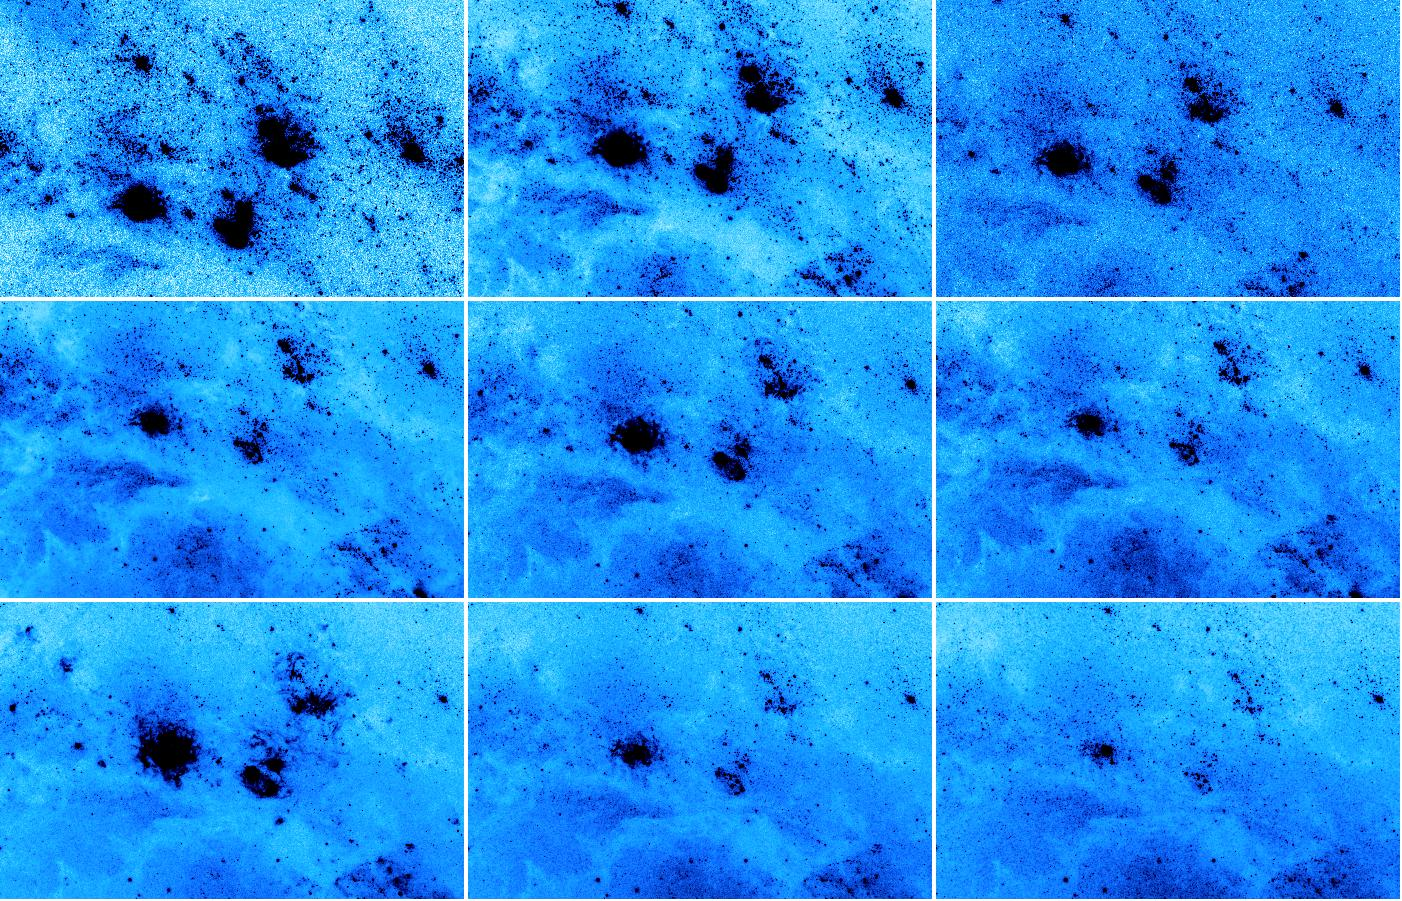
\includegraphics[width=0.87\textwidth]{nine.jpg}
    \caption{Example of how an object can look in 9 wavelenghts}
    \label{fig:nine}
\end{figure}

\subsection{Topics you should review}\index{Related topics}
This will requere a lot of work, but hey it will be worthy and fun!
\begin{itemize}
	\item Astroinformatics and computer science
    	\begin{itemize}
        	\item Data minig
            \item Machine Learning
            \item Big Data Analysis
            \item Neural Networks
            \item Visualization Resources
        \end{itemize}
    \item Statistics and Image Processing
    	\begin{itemize}
        	\item Probability Density Function
            \item Point Spread Function
            \item Full width at half maximum
            \item Convolution
        \end{itemize}
    \item Interstellar medium and star formation
    	\begin{itemize}
        	\item HII regions
            \item Planetary Nebulae
            \item Supernova Remnants
            \item Molecular Gas
            \item All kinds of Nebulae (e.g. dark, refletion)
            \item AGN's (Active Galactic Nucleus)
        \end{itemize}
    \item Astrophysics
    	\begin{itemize}
        	\item Units (light-years, parsecs)
            \item World coordinate system
        	\item Light
            \item Telescopes
            \item Stars and Stellar Evolution
            \item Distance, Brightness, Luminosity
            \item Galaxies
        \end{itemize}
\end{itemize}
The GitHub page will certainly help you to understand why you need to learn about that, and where to find articles, wepages and books.
\subsection{Downloading}
First, let's equip ourselves with the basic software you will need in order to start then you may probably find other cool programs and later you will install them. There is also the possibility that your assigned computer will have them installed already but here is a brief description of what you can do with them, most of them are easy to use.

\begin{description}
	\item[DS9:] It is a program that visualizes astronomy images in FITS format (don't worry if you recognize this format, it will be explained later), where you can easily manipulate them, read their headers, compare, look at regions, see their characteristics, make graphs, even movies. Well, depending on what you need to use later you will be finding all the functions, the best way is to click everywhere and find out what happens, also you can ask to your astronomy colleagues they will tell you all the perks, or if you like learning by yourself or you need someting specific check the documentation webpage. It is faily easy to install, just follow the instructions.
    	\begin{description}
        	\item[Download: ]\url{http://ds9.si.edu/site/Download.html}
            \item[Documentation: ]\url{http://ds9.si.edu/site/Documentation.html}
        \end{description}
        The picture below shows (Fig.\ref{fig:screen}something cool you can do in DS9.
        \begin{figure}[h]
        	\centering
    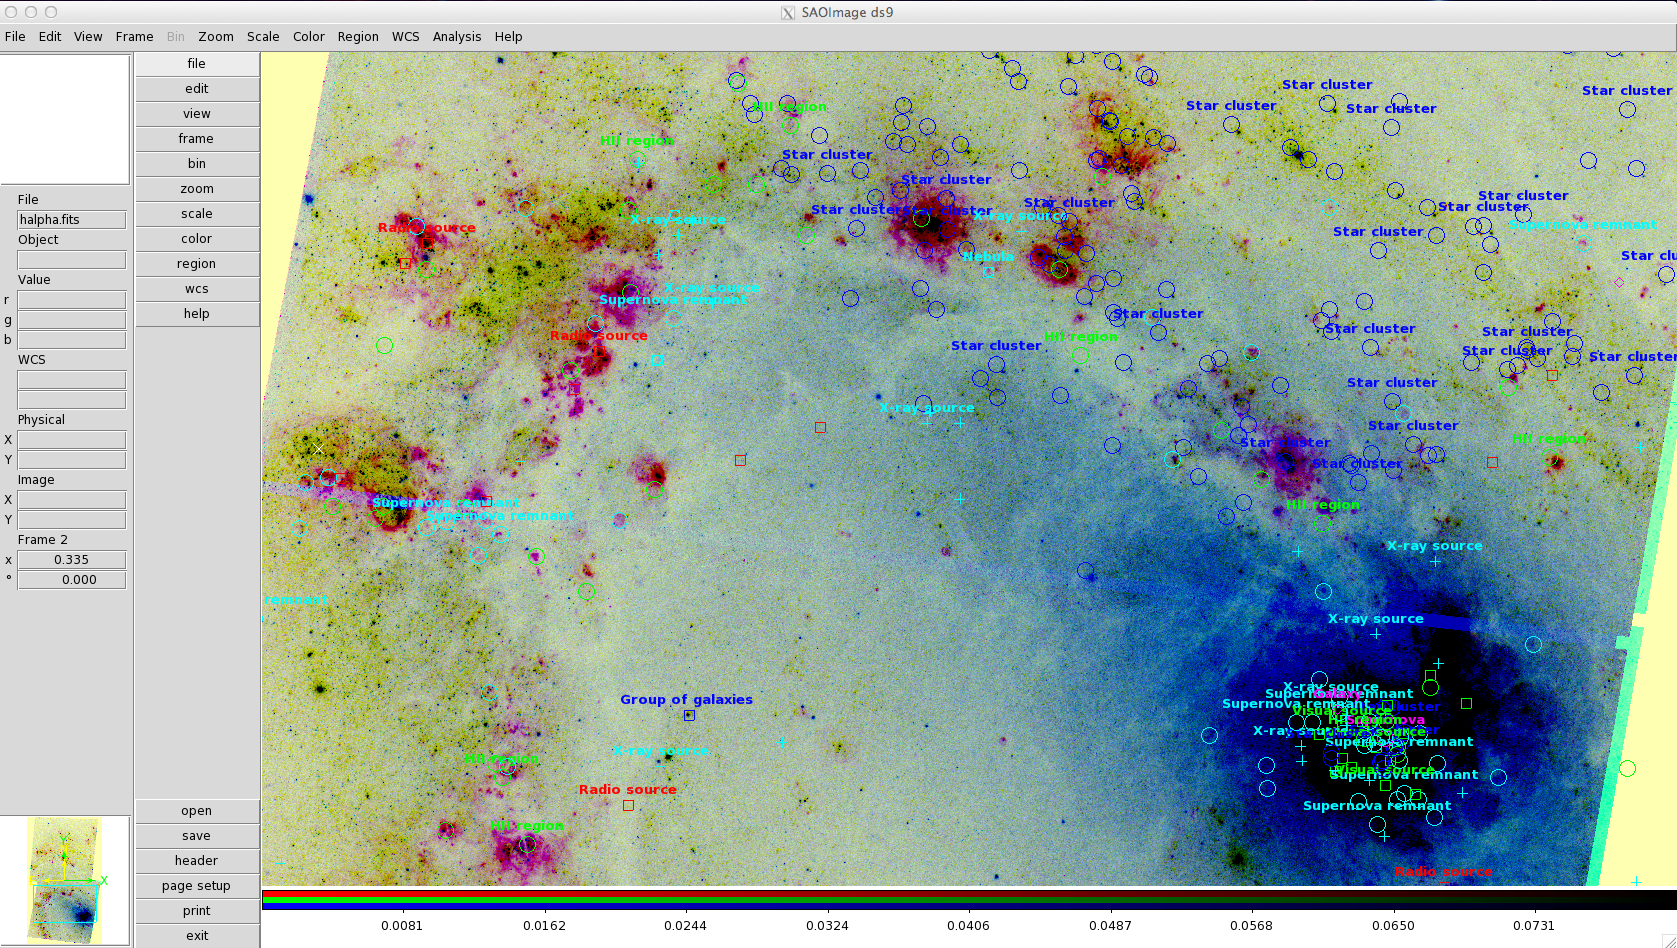
\includegraphics[width=0.87\textwidth]{Screenshot.png}
    \caption{This is an RGB picure made from 3 independent FITS files, with a zscale and a region file overlaid from NED database, if you would like to learn more about this, or reproduce it, it is all explained in this webpage: \url{https://github.com/LaurethTeX/Clustering/blob/master/NEDtoREGION-FILE/KnownRegions.md}}
    \label{fig:screen}
        \end{figure}
        
    \item[Python and a user interface: ]The most \emph{limitless} and user fiendly way to develop programs in Astronomy is using Python, there are many packages, modules, functions now available to help you in almost anything. Me, as an undergrad engineer I'm used to program on an user interface and not directly in a terminal. So, here I will explain you my own way of doing things.
    
    I make my programs on the Canopy editor, it shows when and where you have programing error and warnings, and the interface is easy to learn, now to run, I open a terminal, go to the directory where my program is, type \verb|ipython| wait and then type \verb|run| \verb|myProgram.py|, and wait for the result.
    
    Now there are a lot of fancier ways to work with \emph{Python}, you can program and test directly using \emph{IPython Notebook} on a web broswer or you can just go for the terminal, use \emph{nano} or \emph{vi} or the text editor you like and then run it by typing \verb|python| \verb|myProgram.py|. At this point is up to you, but hey here are some links to start and the packages/modules you should install.
    
    \begin{description}
    	\item[Interfaces or Development environments]\hfill
        	\begin{itemize}
            	\item PyCharm, it a development environment, just like CodeBlocks or NetBeans \url{http://www.jetbrains.com/pycharm/}
                \item Spyder, actually this is the interface that comes with the Python discritution Anaconda, you will get the Python districution and the intrerface. \url{https://store.continuum.io/cshop/anaconda/}
                \item Canopy, this is the one I mentioned before, it super easy to use and you can install packages with one click. \url{https://www.enthought.com/products/canopy/}
            \end{itemize}
        \item[Modules]\hfill
        \\
        In Python, modules are like the libraries in C, therefore, to use math, astronomy and computer science tools you need to install them. To learn whether you already have a module installed or not, type on \emph{iPython} \verb|import andreaModule|, if the output result is something like \verb|ImportError: No module named andreaModule|, you definitely don't have it installed. 
        
        The strategy here to install packages it fairly easy, find their website, go to the download section and follow the instructions, almost all the packages are available on the Python Packaing Index and may be installed by running:
        \begin{verbatim}
        	pip install pyfits
        \end{verbatim}
        To learn how to use them check the documentation page, user manuals or their API's, if you have experience on object oriented programing it will be like running a new bike and if you don't, don't worry too much, Python was designed to be easy to program, just learn the rules of the game.
        	\begin{itemize}
            	\item Astropy, this package is the \emph{must have} of every astronomer, contains tools to handle coordinate systems, units, convolution.. well is better if you take a look at the webpage. \url{http://www.astropy.org/}
                \item Numpy, this package contains the math magic functions, linear algebra tools and the array management variables, make sure you learn all about \emph{Numpy arrays} you will work with them all the time. \url{http://www.numpy.org/}
                \item SciPy, well this package is the base of all scikit modules which contain the functions you will use in image processing and machine learning. \url{http://www.scipy.org/}
                	\begin{itemize}
                    	\item Scikit Image, contains image processing tools, it is the \emph{OpenCV} for \emph{Python} \url{http://scikit-image.org/}
                        \item Scikit Learn, contains data mining algorithms, pretty much contains everything that you will ever need. \url{http://scikit-learn.org/}
                    \end{itemize}
                \item Matplotlib, this package is probably one of the most powerful tools visualize data, you can draw almost anything you want and exacly how you want it. An example of that are the images of the AstroML book, you can access to the image library code and learn how they are made, this is the website \url{http://www.astroml.org/book_figures/index.html}.\footnote{Statistics, Data Mining, and Machine Learning in Astronomy book, it was mentioned before}. You can download the package here \url{http://matplotlib.org/}.
                \item PyFITS, in this package you will find tools to manipulate FITS files, create new ones, create image cubes, tables, and do all kinds of things with their headers. Certainly this package is more than useful. \url{http://www.stsci.edu/institute/software_hardware/pyfits}
            \end{itemize}
    \end{description}
    In the path of researching I'm certain you will find more and new packages and by them you will be prepared to install anything.
    \item[Montage: ]This is a toolkit for assembling astronomical images into mosaics, but it has more functions that you may need in the future to prepare your data before processing it. There are two ways of installing and I would say that is better to have them both. One is to install the toolkit and anytime you need it, you run the commands on the terminal, the other one is to install a \emph{Python} module and use it just like any other module.
    To install montage for terminal, download the lastest version in this website \url{http://montage.ipac.caltech.edu/docs/download.html}, \textbf{read the README file} or go to this website \url{http://montage.ipac.caltech.edu/docs/build.html} and follow the steps, now if you don't have any problem installing it, you can try testing it with an example program found on this website \url{http://montage.ipac.caltech.edu/docs/pleiades_tutorial.html}, in case you are having trouble and your computer is a MAC, instead of doing step five (\emph{If you want to be able to run the Montage executables from any directory}), try this:
    
    \begin{enumerate}
    	\item Open a file called \verb|.profile| located in your user folder. (e.g. \verb|/Users/Laureth|)
        	\begin{verbatim}
            	$ vi .profile
            \end{verbatim}
         \item Include in the file the following
           \begin{verbatim}
           	export PATH=/Applications/Montage_v3.3/bin:$PATH
           \end{verbatim}
           In this link (\url{https://github.com/LaurethTeX/Clustering/blob/master/Tools.md#the-profile-file}) you will find an example of how this file should look. After you modify it, make sure that you save it and type in \verb|/Users/Laureth|,
           \begin{verbatim}
           	$ source .profile
           \end{verbatim}
           Then try testing the \emph{Montage} commands, and I'm sure that it will magically work, just remember that anytime you use any command, type \verb|source .profile|.\\
            
    \end{enumerate}
    
    
    
      Now the other way to install, implies only to install a \emph{Python} module but this module contains less functions that the terminal application, in any case check the website \url{http://www.astropy.org/montage-wrapper/}, there you will find all the documentation you may need and the instructions to install it (\emph{Spoilers} \verb|pip install montage-wrapper| ).\\
\end{description}

Any questions you may have and how to install, here is my GitHub page for software tools \url{https://github.com/LaurethTeX/Clustering/blob/master/Tools.md}

%----------------------------------------------------------------------------------------
%	CHAPTER 3
%----------------------------------------------------------------------------------------

\chapterimage{boat.png}
\chapter{Understand your data}

Before continuing, first and most importantly you must select the \emph{raw} data you are going to process and later after you aquire experience with an specific dataset the idea is to expand the algorithms to any kind of dataset. The important things are to learn how to input the data correctly, establish the right \emph{learning paramenters} in the selected algorithm and find the best way to visualize your results and interpret them correctly.

Now let's start with basic concepts that vary from an engineering to an astronomer point of view.
\section{What is an image?}
	As you may know, an image is a matrix of numbers that cointains the specific brightness level that corresponds to a given pixel. And from there the concepts evolves and adds channels of colour and depth. But for now, let's just think about monochromatic images (only one channel). In Astronomy, images are usually considered sets of scientific data, observations, that contain information about an speficic target in the sky seen throught an specific filter and the levels of brightness correspond to the behaviour of the optical sensor (CCD camera) in relation with the number of electrons that hit a particular pixel through an specific waveband. Something else to consider is that the sky is not flat with this I mean that the celestial vault is like a sphere surrounding us therefore cartesian coorditanes are not the paramenters used to identify points in space, there is another system called WCS (World Coordinate System) hence a conversion between pixels and WCS coordinates exists. As you are realizing now just one image can contain tons of information related to it, now imagine that multiplied for terabytes and terabytes of stars, galaxies, planets, nebulae or any object in space. Fortunately in astronomy this is solved using an image format that cointains the image and its own information.
	\subsection{FITS files}
    	This format is the standard data format used in astronomy, can contain one image, multiple images, tables and header keywords providing descriptive information about the data. The way it works is that this format can contain a text file with keywords that comprise the information about the observation and a multidimensional array that could be a table, or an image, or an array of images (data cube). This files can be managed in diffetent ways, with an image preview use DS9, for handing the data in a program use the \emph{Python} package \emph{PyFITS}.
        
	\subsection{WFC3 ERS M83 Data Products}
    The selected dataset to test the data mining libraries I found is a series of observations of M83 at 9 different wavelengths, the original images can be found in this webpage, \url{http://archive.stsci.edu/prepds/wfc3ers/m83datalist.html}, the specific information about them can be found in Table \ref{tab:uno}. This particular images were observed through HST with the WFC3/UVIS camera.
    
\begin{table}[h]
  \centering
  \begin{tabular}{ c c c c c c }
    \hline\hline
    Filter / Config. & Waveband / Central $\lambda$/ Line & Obs. Date & Comment \\
    \hline
    F225W & UV filter / 235.9 nm & 26 Aug 2009 &  UV wide\\
    
    F336W & UV filter / 335.5 nm & 26 Aug 2009 & Str$\ddot{o}$mgren $u$\\
    
    F373N & Narrow-Band Filter / 373.0 nm & 19 Aug 2009 & Includes \textsc{[OII]}\\
    
    F438W & Wide-Band Filter / 432.5 nm & 26 Aug 2009 & $B$, Johnson-Cousins set\\
    
    F487N & Narrow-Band Filter / 487.1 nm & 25 Aug 2009 & Includes H$\beta$\\
    
    F502N & Narrow-Band Filter / 501.0 nm & 26 Aug 2009 & Includes \textsc{[O III]}\\
    
    F657N & Narrow-Band Filter / 656.7 nm & 25 Aug 2009 & Includes H$\alpha$+\textsc{[NII]}\\
    
    F673N & Narrow-Band Filter / 676.6 nm & 20 Aug 2009 & Includes \textsc{[SII]}\\
    
    F814W & Wide-Band Filter / 802.4 nm & 26 Aug 2009 & $I$, Johnson-Cousins set\\
    \hline
  \end{tabular}
  \caption{Summary of Observations}
  \label{tab:uno}
\end{table}
%Poner aqui la tabla con los datos de acada filtro
%No olvidar poner en GitHub el programa de como hacer el cube y tammbien el de reproject cube con montrage wrapper

\section{Preprocessing your data}
This section is where you prepare your data to be processed, you have to make sure that all your images have the same grid size, same spatial resolution, less possible quantity of outliers abd noise and same coordinate system. Now, what are those things? Same grid size means that your images must have the same pixel size, in the dataset we are processing we don't have to worry about this, the pixel size is 0.0396 arcsec/pixel. Now, spatial resoultion, each image has it's own spatial resolution depending on the filter that was used to get the observation, the number that you will be looking for is the FWHM that describes the PSF of every image. When you have all the FWHM for all the images you should choose the largest which corresponds to the poorest spatial resolution and create a convolution kernel with \emph{Tiny Tim} or use a gaussian kernel calculated with \emph{Astropy} and convolve all the images with that kernel. This exactly what I did, if you look at image \ref{img:conv}, you will see the before and after convolution. In table \ref{tab:dos} you can see how I chose the number for the FWHM.

\begin{figure}[h]
	\centering
    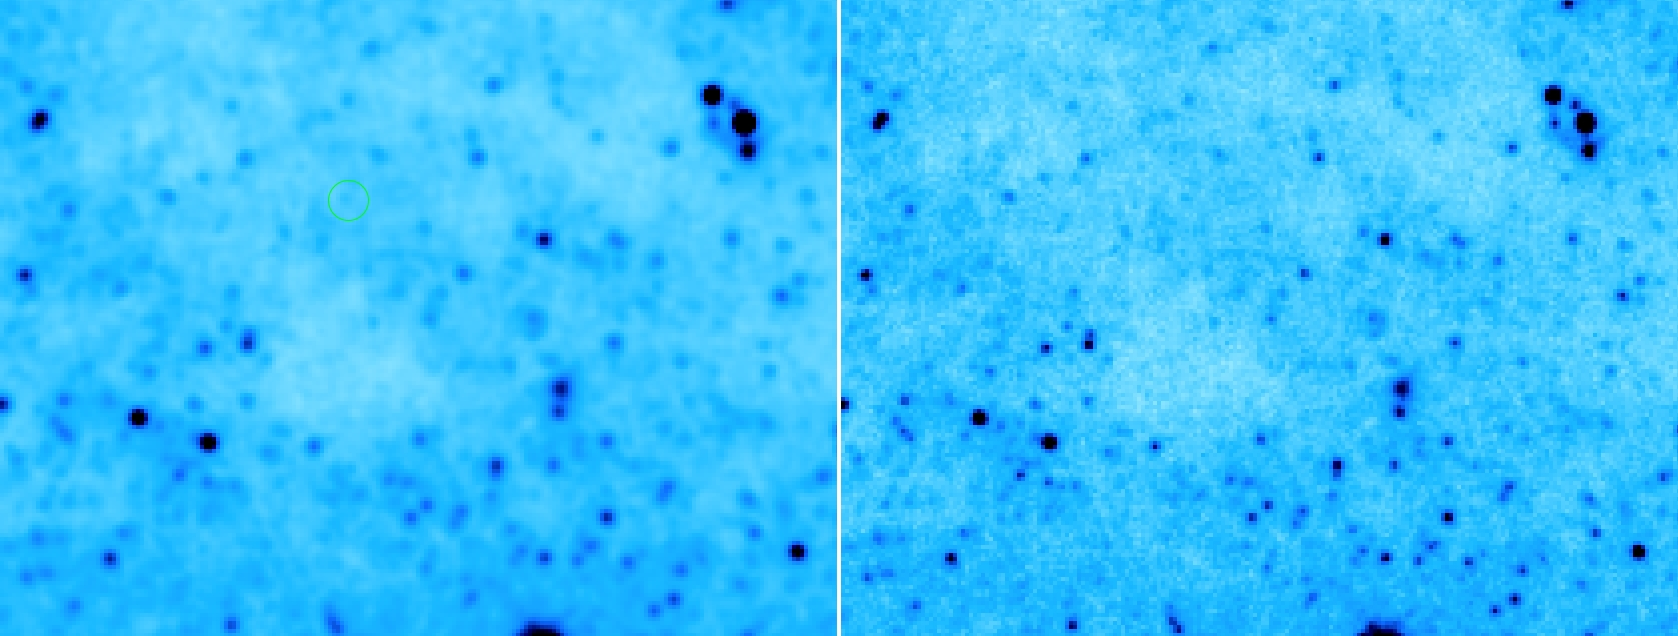
\includegraphics[width=0.87\textwidth]{conv.jpg}
    \caption{In this image you can observe how an observation looks, before and after convolution, this particular image corresponds to the B band filter and was convolved to a 0.083 arcsec FWHM}
    \label{img:conv}
\end{figure}

\begin{table}[h]
  \centering
    \begin{tabular}{ c c c }
    \hline\hline
    
    Filter / Config. & Central $\lambda$ & FWHM (arcsec)\\
    \hline
    
    F225W & 235.9 nm & $\sim$0.083\\
    
    F336W & 335.5 nm & $\sim$0.075\\
    
    F373N & 373.0 nm & $\sim$0.070\\
    
    F438W & 432.5 nm & $\sim$0.070\\
    
    F487N & 487.1 nm & $\sim$0.067\\
    
    F502N & 501.0 nm & $\sim$0.067\\
    
    F657N & 656.7 nm & $\sim$0.070\\
    
    F673N & 676.6 nm & $\sim$0.070\\
    
    F814W & 802.4 nm & $\sim$0.074\\
    
    \hline
  \end{tabular}
  \caption{WFC3/UVIS PSF FWHM informations for the selected dataset, as you can see the largest number here is 0.083 wich means the poorest spatial resolution, this is the number used to calculate the convolution kernel, in order to precess them all images must have the same spatial resolution.}
  \label{tab:dos}
\end{table}

After convoling all the picures, I started to do some tests, but I realized that maybe around 30\% of the images was missing information and/or noise and the results I was getting were mislead by the outliers. In clustering algorithms we must help the algorithm, make sure that what we are inputing is something that can be clustered, although some of them are \emph{shielded} against outliers, making our data more accesible and easy for the neural networks to interpret will help you to get better results, as you can see in image \ref{img:dos} (open one and explore it in DS9) there is missing information and noise. In order to correct this I decided to go with the easiest way I could think of, just cut the image. And I did selected a processable area excluding all the missing information and noisy areas.

\begin{figure}[h]
	\centering
    \includegraphics[width=0.47\textwidth]{uno.jpg}
    \caption{Look at the image, it is composed of two mosaics, therefore, there are some regions with missing data, now look at the borders of each mosaic there is noise near the edges, this is data that we don't want messing with our clustering algorithm and can be classifed as outliers, it is very important to reduce them as much as possbile so the output clusters can be correclty classified and correspond to the information that we are looking for}
    \label{img:dos}
\end{figure}

The next step was to build the datacube, at this point you can decide if you want to process your images indendently or all of them. The ideal here is to input all of them in a datacube, so the output cluters relate information from all the wavelenghts and the regions covered by them can be interpreted more easily. Now if you choose to create an imagecube (just append the image arrays in one FITS file) it is posible that youy images have a different conversion between their world coordinate system to pixel, so have to make sure all of your images are projected with only one conversion, this mean that you have to reproject them to a common WCS.

Well, what I wrote before it is a brief summary of what I did, but I'm sure that you can find a better way to do your own data pre-processing but here are some things that you should consider:
	\begin{itemize}
    	\item Create a methond as general as possible, with input parameter that can be adapted to any kind of data, this will save you a lot of work in the future
        \item Understand first your algorithm, how the data is going to be processed and design the best way to input your data
        \item Accomodate your data according to the type of attributes that the algorithm can handle
        \item Consider the size of your dataset, if it's huge your program may never end
        \item Find out of your algorithm can work with high dimensional data (multi-wavelenght), because if not, you won't be able to input datacubes
        \item Find out if your selected clustering algorithms is able to find clusters of irregular shapes, this will help you to device the best way to accomodate your patterns
        \item Handle outliers, if you identify them, know where they are, try to eliminate them as much as possible, we don't want them messing with our clusters
        \item In case that you come up with an artful mathematical method like PCA to reduce dimensionality, make sure that what you input can later make sense when is clustered, becuase you will be working in another space
        \item Remeber that the most important goal is to find hidden knowledge therefore, you must know you to visualize and interpret your results
        \item For the let's call it \emph{astronomy image processing}, make sure that your data is scientifically aproved ask people around you.
    \end{itemize}

%Convolution
%Cropping
%Repgojection
%Cubbing
%Explain the main rules of why to preprocess the data

This section is explained at lenght in the GitHub page, there you will find my codes and some helpful links, \url{https://github.com/LaurethTeX/Clustering/blob/master/Preprocessing.md}

\section{Software available}
%Como hacer preprocessing en los datos
For doing data preprocessing there are a bunch of softwares available, even there is one being developed by Sophia Lianou called \emph{imagecube} which, when it is finished, will be one of the best, has everything you need in one package. I'll say that this part is yours to discover, everyday there are more and more being released or new versions of the existent ones but in the meanwhile it will depend entirely on you, which software you want to use. For \emph{Python} all the functions you will need can be found in the \emph{Astropy} module, \textbf{check the API!!!.}


This specific part is all explained in GitHub in this link. \url{https://github.com/LaurethTeX/Clustering/blob/master/Preprocessing.md#first-step-data-pre-processing}

\begin{remark}
	Some links to start,
    \begin{itemize}
    	\item Astropy, Convolution and filtering, \url{http://docs.astropy.org/en/stable/convolution/index.html}
        \item AstroDrizzle: New Software for Aligning and Combining
HST Images, With Improved Handling of Astrometric Data, \url{http://drizzlepac.stsci.edu/}
		\item Tiny Tim HST PSF Modeling, \url{http://www.stsci.edu/hst/observatory/focus/TinyTim}
        \item IRAF, Image Reduction and Analysis Facility, \url{http://iraf.noao.edu/}
    \end{itemize}
\end{remark}


%----------------------------------------------------------------------------------------
%	CHAPTER 4
%----------------------------------------------------------------------------------------

\chapterimage{head1.png} % Chapter heading image

\chapter{Experimenting}

I discovered surfing on the internet a cloud computing software that is free, has data mining algorithms embeded, is specifically developed for Astronomy and is programmed by Caltech, University Federico II and the Astronomical Observatory of Capodimonte. The homepage website, \url{http://dame.dsf.unina.it/index.html}. Well, the platform for testing is ready!, now what? I requested and account and the next day they sent me an acceptance with my username and my password approved.
I introduced myself to the documentation, the available clustering funcionts, the manuals for every method, the blogs and discovered that the was one method available that could work with datacubes and do its clustering on every pattern (number in the multidimensional matrix) which was exaclty what I needed. The name of this method is ESOM (Evolving Self Organizing Maps) and I read its manual, did some foolish test with all my image and ... never got a result ... the experiment ran forever (more than two weeks), when I realised that this wasn't the best way to tackle this problem I started considering only clustering on the independent images and not in the datacube due to the fact that the dimensionality was inmense. So, in the end my selected methods have some results but not all, here is where all the work has to be done, analyzed and tested again.

\section{Methods Selected}

\subsection{ESOM, Evolving Self Organizing Maps}
The \emph{official} manual for this method can de found here, \url{http://dame.dsf.unina.it/documents/ESOM_UserManual_DAME-MAN-NA-0021-Rel1.2.pdf}, there you will find a full explanation of the method, the meaning of every variable and the supported file types.

Here is my own explanation of how this particular method works, first of all, can be used as an unsupervised machine learning technique or you can help the algorithm to identify regions an make it a supervised machine learnig technique, this type of clustering finds groups of patterns with similarities and preserves its topology, starts with a null network without any nodes and those are creted incrementally when a new input pattern is presented, the prototype nodes in the network compete with each other and the connections of the winner node are updated. 

The method is divided in three stages, \emph{Train}, \emph{Test} and \emph{Run}.
The first step to experiment with this method is Train. Here, the important variables to undertand an look at are, the learning rate, epsilon and the pruning frequency. It is highly recomendable that you check the DAMEWARE manual for this function, there they will explain in detail the meaning of each on the mentioned variables.
% fULL AND SAMPLE DATACUBE
\subsubsection{Expected Results}
	This particular method as I mentioned before supports datacubes and considers as an independent pattern all the  numbers in the multi-dimensional array this means that our clusters are groups of patterns with similar characteristics, that correspond to volumes of similar fluxes of electrons inside the datacube.
    
    The output files from the experiment that will show us our results are, 
    \begin{itemize}
    	\item \emph{E\_SOM\_Train\/Test\/Run\_Results.txt}: File that, for each pattern, 
reports ID, features, BMU, cluster and activation of winner node
		\item \emph{E\_SOM\_Train\/Test\/Run\_Histogram.png}: Histogram of clusters found 
        \item \emph{E\_SOM\_Train\/Test\/Run\_U\_matrix.png}: U-Matrix image 
        \item \emph{E\_SOM\_Train\/Test\/Run\_Clusters.txt}: File that, for each clusters, reports label, number of pattern assigned, percentage of association respect total number of pattern and its centroids. 
        \item \emph{E\_SOM\_Train\_Datacube\_image.zip}: Archive that includes the 
clustered images of each slice of a datacube.\footnote{I have my doubts whether this file is produced or not, in none of my test was produced, you might need to contact the developers and ask about this.}
    \end{itemize}
The file that you will be looking forward to see is the last one, the zip where you will be able to see the slices of the volume, and how the final configuration of the clusters was arranged.

\subsubsection{Failed and still running tests: What no to do and what is still running}
The first tests I did included all the complete datacube, including the areas where data was missing, the images were only reprojected and convolved. That was before realising that outliers migth affect the ability of the algorithm to identify the clusters and distract them with noise and missing data. So, the first thing you must NOT do, is to get rid of the outliers when you are training your network, if you ever get to have a well trained network then it might be interesting to learn how the network interacts with noise an outliers, but for now we will help her a bit. 

In table \ref{tab:ds9failed} are the input parameters I used to the failed tests applied in the \emph{raw} datacube, and in table \ref{tab:ds9running} are the input parameters used on experimets that are stil running since August 7th, 2014. (I wonder if they will ever end)

\begin{table}[h!]
  \centering
    \begin{tabular}{ c c c c c c }
    \hline\hline
    
    Name & Input nodes & Normalized data & Learning rate & Epsilon & Pruning Frequency\\
    \hline
    
    Train2 & 1 & 1 & 0.3 & 0.001 & 5\\
    Train3 & 1 & 1 & 0.7 & 10 & 100\\
    Train4 & 1 & 1 & 0.95 & 1 & 10\\
    Train5 & 1 & 1 & 0.99 & 0.1 & 10\\
    Train6 & 1 & 1 & 0.01 & 0.01 & 1\\
    Train7 & 1 & 1 & 0.5 & 0.7 & 5\\
    Train8 & 1 & 1 & 0.5 & 0.5 & 7\\
    Train11 & 1 & 1 & 0.25 & 0.00001 & 10\\
    
    \hline
  \end{tabular}
  \caption{This table describes all the failed experiments done in the workspace WFC3 with the \emph{raw} datacube as an input, using the ESOM method in the DAME platform selecting the number 3 as the dataset type and without using a previous configuration file.}
  \label{tab:ds9failed}
\end{table}

\begin{table}[h!]
  \centering
    \begin{tabular}{ c c c c c c }
    \hline\hline
    
    Name & Input nodes & Normalized data & Learning rate & Epsilon & Pruning Frequency\\
    \hline
    
    Train9 & 1 & 1 & 0.3 & 0.0001 & 5\\
    Train10 & 1 & 1 & 0.99 & 0.0001 & 10\\
    Train12 & 1 & 1 & 0.5 & 0.0001 & 5\\
    
    \hline
  \end{tabular}
  \caption{This table describes all the experiments done in the workspace WFC3 that are still running since August 7th, 2014 with the \emph{raw} datacube as an input, using the ESOM method in the DAME platform selecting the number 3 as the dataset type and without using a previous configuration file.}
  \label{tab:ds9running}
\end{table}

Some of the failed experiments had histogram like the one you can see on figure \ref{img:faildtrain2} where the cluters were created but reached a point where the neural network could not define how to differenciate a cluster from another clusted and failed.

\begin{figure}[h!]
	\centering
    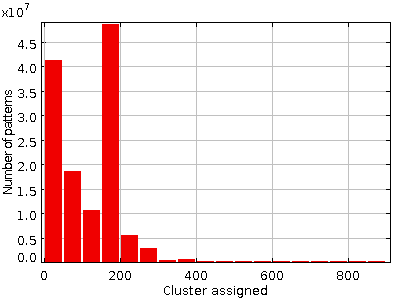
\includegraphics[width=0.47\textwidth]{Histogram_train2.png}
    \caption{In this particular experiment, the neural network failed due to a very low prunning frequency, high number of patterns and all the outliers inclusions.}
    \label{img:faildtrain2}
\end{figure}

Hey, if you were wondering why I always choose to normilize, and one as the input node, well the normalization is due to the fact that I know that the data has, according to its filter, all kinds of ranges of fluxes on every layer which means that the distances between patterns might not be correct, this is a topic you should look into. And for the input node I choose 1 because if I start with any other number the experiment automatically fails, and of course we do not want that.

As I progressed and saw the results and the \emph{log files} in all the failed experiments I decide to try the algorithm on independent layers and see if I could get something. Therefore I selected the H$\alpha$ convolved observation (halpha\_conv.fits) and did some tests on it, table \ref{tab:hafailed} shows the parameters I used for the failed experiments and table \ref{tab:harun} shows the paramters fo the still running experiments.

\begin{table}[h!]
  \centering
    \begin{tabular}{ c c c c c c }
    \hline\hline
    
    Name & Input nodes & Normalized data & Learning rate & Epsilon & Pruning Frequency\\
    \hline
    
    TrainHa1 & 1 & 1 & 0.5 & 0.01 & 5\\
    TrainHa2 & 1 & 1 & 0.5 & 0.001 & 5\\
    
    \hline
  \end{tabular}
  \caption{This table describes the failed experiments done in the workspace WFC3 for the \emph{halpha\_conv.fits} file, using the ESOM method for one layer in the DAME platform selecting the number 3 as the dataset type and without using a previous configuration file.}
  \label{tab:hafailed}
\end{table}

\begin{table}[h!]
  \centering
    \begin{tabular}{ c c c c c c }
    \hline\hline
    
    Name & Input nodes & Normalized data & Learning rate & Epsilon & Pruning Frequency\\
    \hline
    
    TrainHa3 & 1 & 1 & 0.5 & 0.0001 & 5\\
    
    \hline
  \end{tabular}
  \caption{This table describes the still running experiments since August 10th, 2014 in the workspace WFC3 for the \emph{halpha\_conv.fits} file, using the ESOM method for one layer in the DAME platform selecting the number 3 as the dataset type and without using a previous configuration file.}
  \label{tab:harun}
\end{table}

My next mental step was to repeat the tests eliminating as many outliers I could reduce, my hypothesis here is that, if I elimante all the areas where there is missing data and noise, the neural networks will be concentrated only in the patterns I'm interested in clustering and maybe idenfying interesting regions that correspond to some known interstellar object. So, what I did was to try the ESOM algorithm with, again, independent images, this time I decided to apply the same experiment to three different layers, H$\alpha$, UV wide and $i$-band. In table \ref{tab:threefail} you can see the parameters of the failed experiments and on figure \ref{img:fail3} there are some of the output histograms. Also, in table \ref{tab:threerun} you can see the input parameters of the still running experiments.

\begin{table}[h!]
  \centering
    \begin{tabular}{ c c c c c c }
    \hline\hline
    
    Name & Input nodes & Normalized data & Learning rate & Epsilon & Pruning Frequency\\
    \hline
    
    Train1 & 1 & 1 & 0.5 & 0.001 & 50\\
    Train2 & 1 & 1 & 0.5 & 0.01 & 50\\
    Train3 & 1 & 1 & 0.5 & 0.1 & 100\\
    Train4 & 1 & 1 & 0.5 & 0.001 & 100\\
    
    \hline
  \end{tabular}
  \caption{This parametes where used in three different workspaces (\emph{halphaCrop, uvwidecrop, ibandcrop}), with their own input file that corresponded to the convolved and cropped observation of each filter (halpha\_conv\_crp.fits, uvwide\_conv\_crp.fits, iband\_conv\_crp.fits), all of the experiments had no previous configuration file and the dataset type was 3 and all failed.}
  \label{tab:threefail}
\end{table}

\begin{figure}[h!]
	\centering
    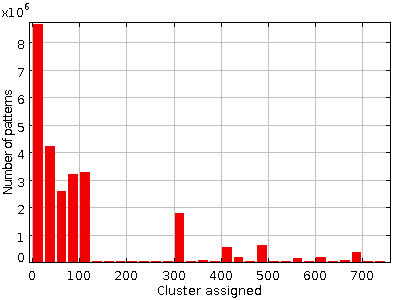
\includegraphics[width=0.31\textwidth]{Histogram-halpha1.png}
    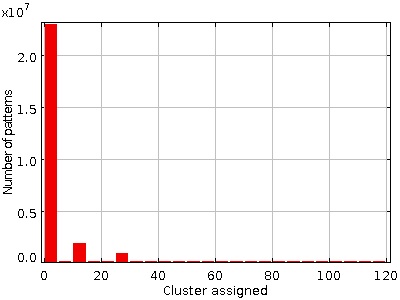
\includegraphics[width=0.31\textwidth]{Histogram-uvwide-2.png}
    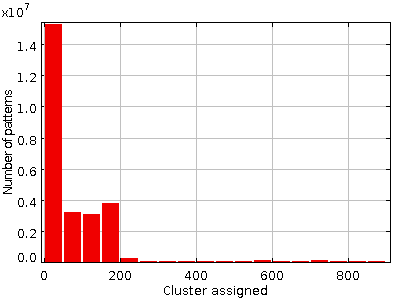
\includegraphics[width=0.31\textwidth]{Histogram-iband3.png}
    \caption{The histogram on the left corresponds to the halpha workspace in Train1, the one on the center to the iband workspace in Train3 and the one on the right to the uvwide workspace in Train2, all of them were failed experiments.}
    \label{img:fail3}
\end{figure}

\begin{table}[h!]
  \centering
    \begin{tabular}{ c c c c c c }
    \hline\hline
    
    Name & Input nodes & Normalized data & Learning rate & Epsilon & Pruning Frequency\\
    \hline
    
    Train5 & 1 & 1 & 0.5 & 0.0001 & 100\\
    Train6 & 1 & 1 & 0.99 & 0.0001 & 75\\

    \hline
  \end{tabular}
  \caption{This parametes where used in three different workspaces (\emph{halphaCrop, uvwidecrop, ibandcrop}), with their own input file that corresponded to the convolved and cropped observation of each filter (halpha\_conv\_crp.fits, uvwide\_conv\_crp.fits, iband\_conv\_crp.fits), all of the experiments had no previous configuration file and the dataset type was 3. The experiments mentioned are still running since August 11th, 2014.}
  \label{tab:threerun}
\end{table}

As you can see, I discovered that if I choose an epsilon of 0.0001 the experiments will be still running, and all of the other variables can be variated like the learning rate and the pruning frequency.

\subsubsection{The big and small reprojected datacube}
After a few days of waiting anxiously for the experiments to end and not getting any new results I decided to test the convolved, cropped and reprojected datacube including all the layers with a fixated prunning frequency of 0.0001, hopping that this time I could get some interesting results. The input parameters for the two experiments I tested can be seen in table \ref{tab:cubeesom}.

\begin{table}[h!]
  \centering
    \begin{tabular}{ c c c c c c }
    \hline\hline
    
    Name & Input nodes & Normalized data & Learning rate & Epsilon & Pruning Frequency\\
    \hline
    
    ESOMtrain1 & 1 & 1 & 0.5/0.75 & 0.0001 & 100\\
    ESOMtrain2 & 9 & 1 & 0.75 & 0.001 & 100\\

    \hline
  \end{tabular}
  \caption{This parametes where used in two different workspaces (\emph{DataCube, RPDataCube}), the first experiment is still running since August 12th, 2014 and the second failed. The input for the DataCube workspace corresponds to a 9 layer datacube with no reprojection and the RPDataCube input is the same datacube but reprojected.}
  \label{tab:cubeesom}
\end{table}

As you can see, in the experiment \emph{ESOMtrain2} I tried to start the neural network with 9 nodes (thinking logically as having 9 layers in the datacube) and immediatly the experiment failed, so \textbf{do not try to input a number different than one.}

I waited 17 days for the experiments to finish (I did some other stuff in the meanwhile, most of the time learning new things) but I did not get any results so I came up with a different strategy, selecting small datacubes with already identified regions by the NED database. I selected randomly a particular HII region located in RA 204.26971, DEC -29.84933 (See figure \ref{img:h2region}) and centered it in a 605x605 pixels sample.

\begin{figure}[h!]
	\centering
    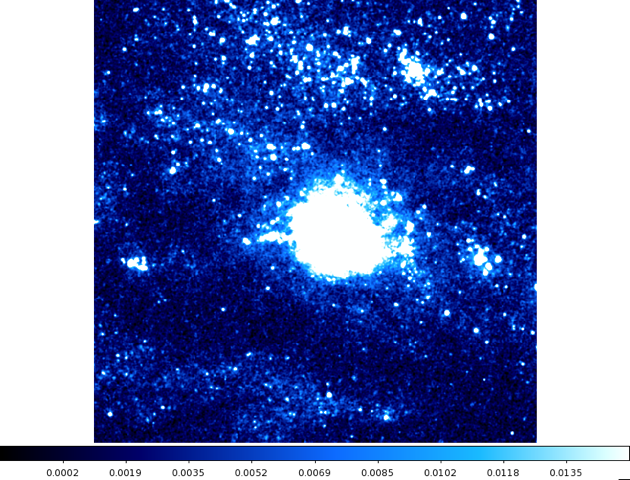
\includegraphics[width=0.52\textwidth]{small_ex.png}
    \caption{Illustration of the randomly chosen HII region for the small sample from the M83 reprojected datacube.}
    \label{img:h2region}
\end{figure}

This time, most of the experiments gave me immediate results failing or finishing. On table \ref{tab:small}, you can see the input parameters and the status of the experiments I tested with the small datacube.

\begin{table}[h!]
  \centering
    \begin{tabular}{ c c c c c c }
    \hline\hline
    
    Name & Normalized & Learning rate & Epsilon & Pruning Frequency & Status\\
    \hline
    
    ESOMtrain1 & 0 & 0.5 & 0.001 & 50 & Running\\
    Train2 & 1 & 0.5 & 0.0001 & 50 & Ended\\
    Train3 & 1 & 0.5 & 0.1 & 50 & Ended\\
    Train4 & 0 & 0.5 & 0.0001 & 50 & Running\\
    Train5 & 0 & 0.95 & 0.0001 & 100 & Running\\
    Train6 & 1 & 0.99 & 0.001 & 50 & Ended\\

    \hline
  \end{tabular}
  \caption{All the mentioned experimend belong to the SmallDataCube workspace, have 3 as data type and one input node, no previous configuration file and the input file is \emph{rp\_small\_datacube.fits}.}
  \label{tab:small}
\end{table}
In this case three of the experiments ended and none od them failed (yet), here I detected that the output file that contains the distributions of the clusters on every layer is missing, but we got some interesting resuts, in the next figures (\ref{img:smallended},\ref{img:matrixended}) you can apreciate better what I'm taking about.

\begin{figure}[h!]
	\centering
    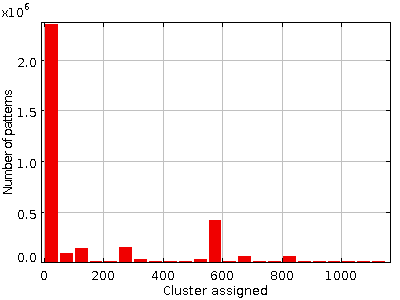
\includegraphics[width=0.31\textwidth]{Small-train2.png}
    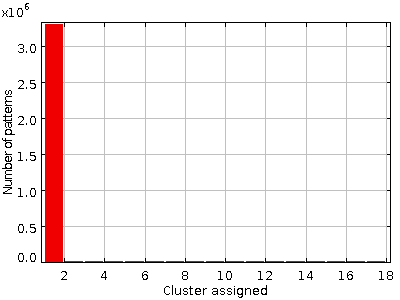
\includegraphics[width=0.31\textwidth]{Small-train3.png}
    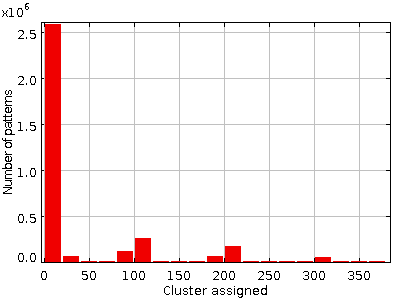
\includegraphics[width=0.31\textwidth]{Small-train6.png}
    \caption{All of the images correspond to histograms of the ended experiments mentioned above in order (Train2, Train3, Train6), as you can see there is a predominance on one of the clusters that can mean that is detecting the HII region or the experiment never started, to understand further the results a visualization of the clusters is needed.}
    \label{img:smallended}
\end{figure}

\begin{figure}[h!]
	\centering
    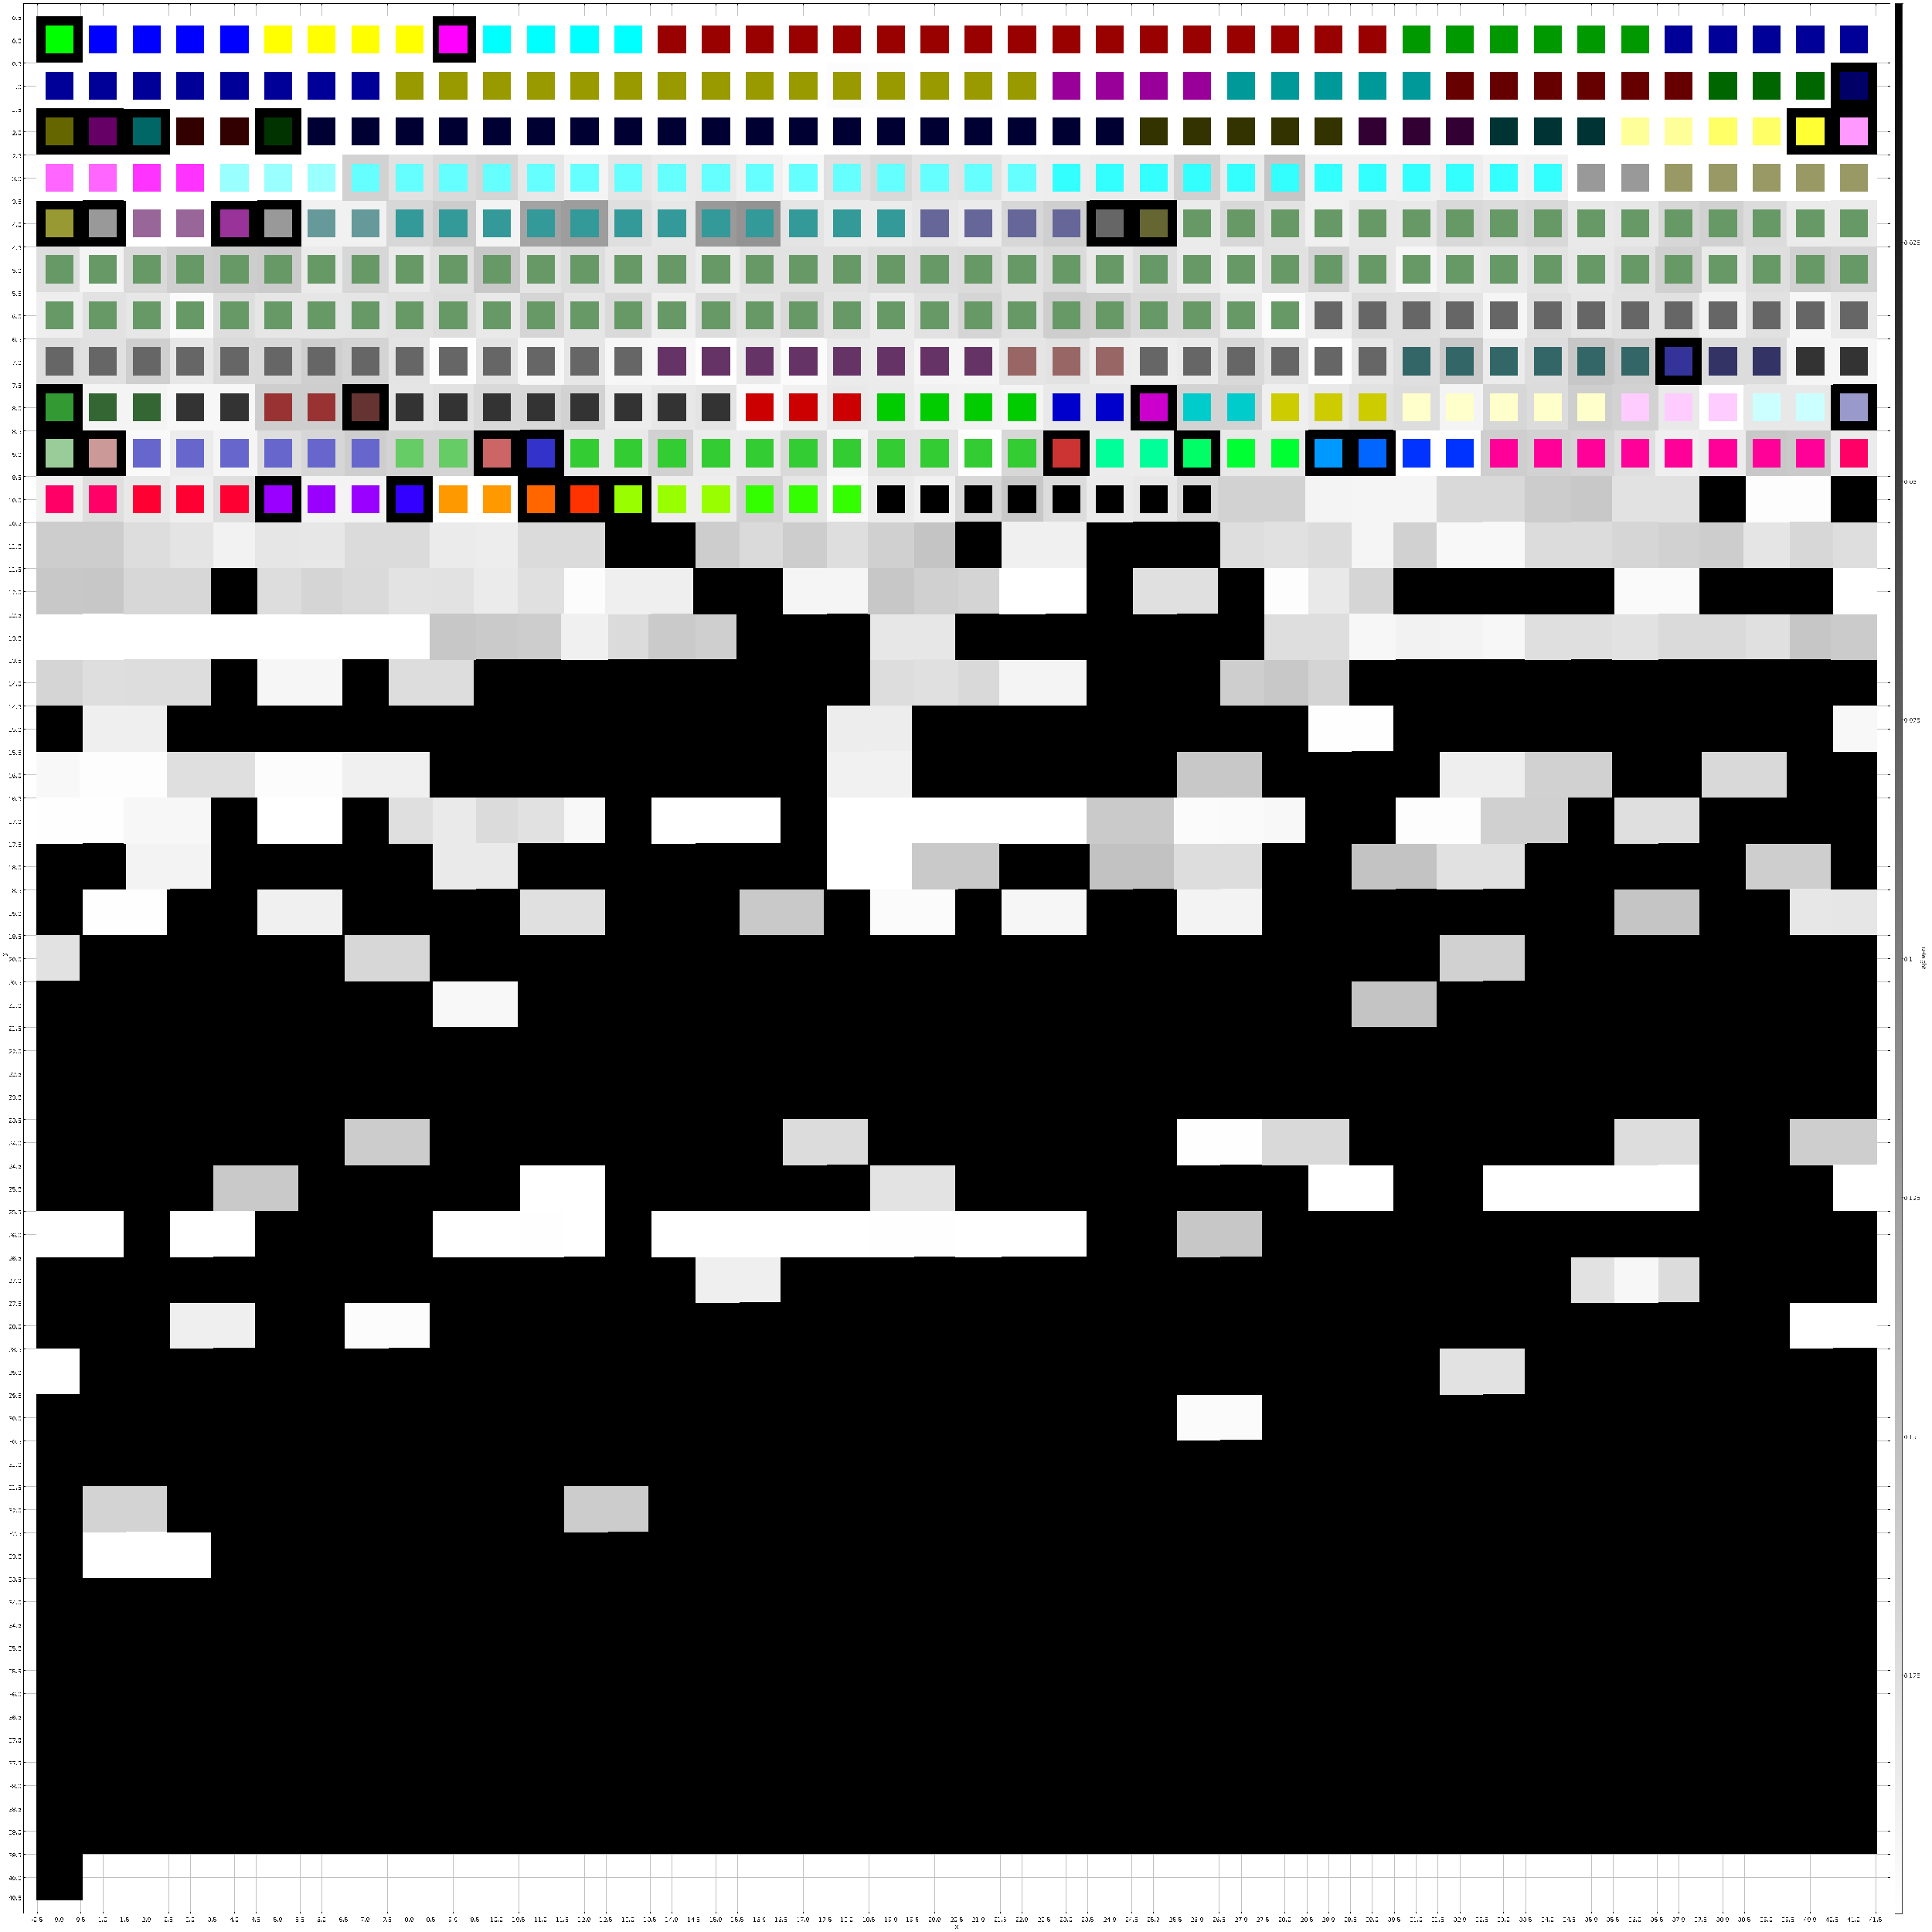
\includegraphics[width=0.31\textwidth]{matrix2-01.png}
    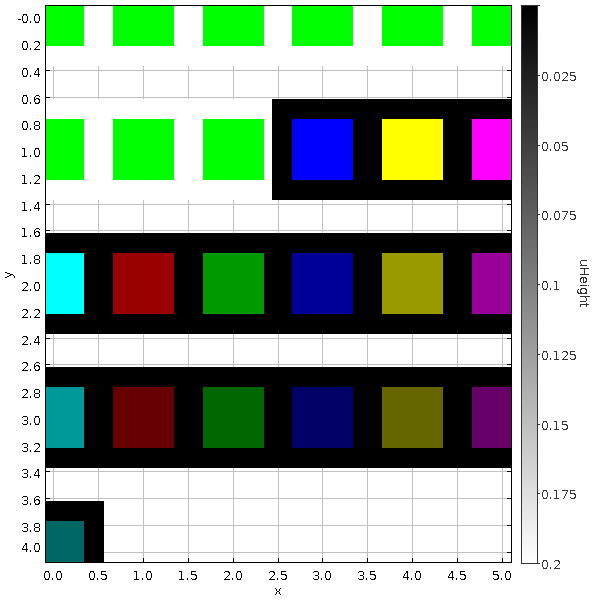
\includegraphics[width=0.31\textwidth]{Small-train3-matrix.png}
    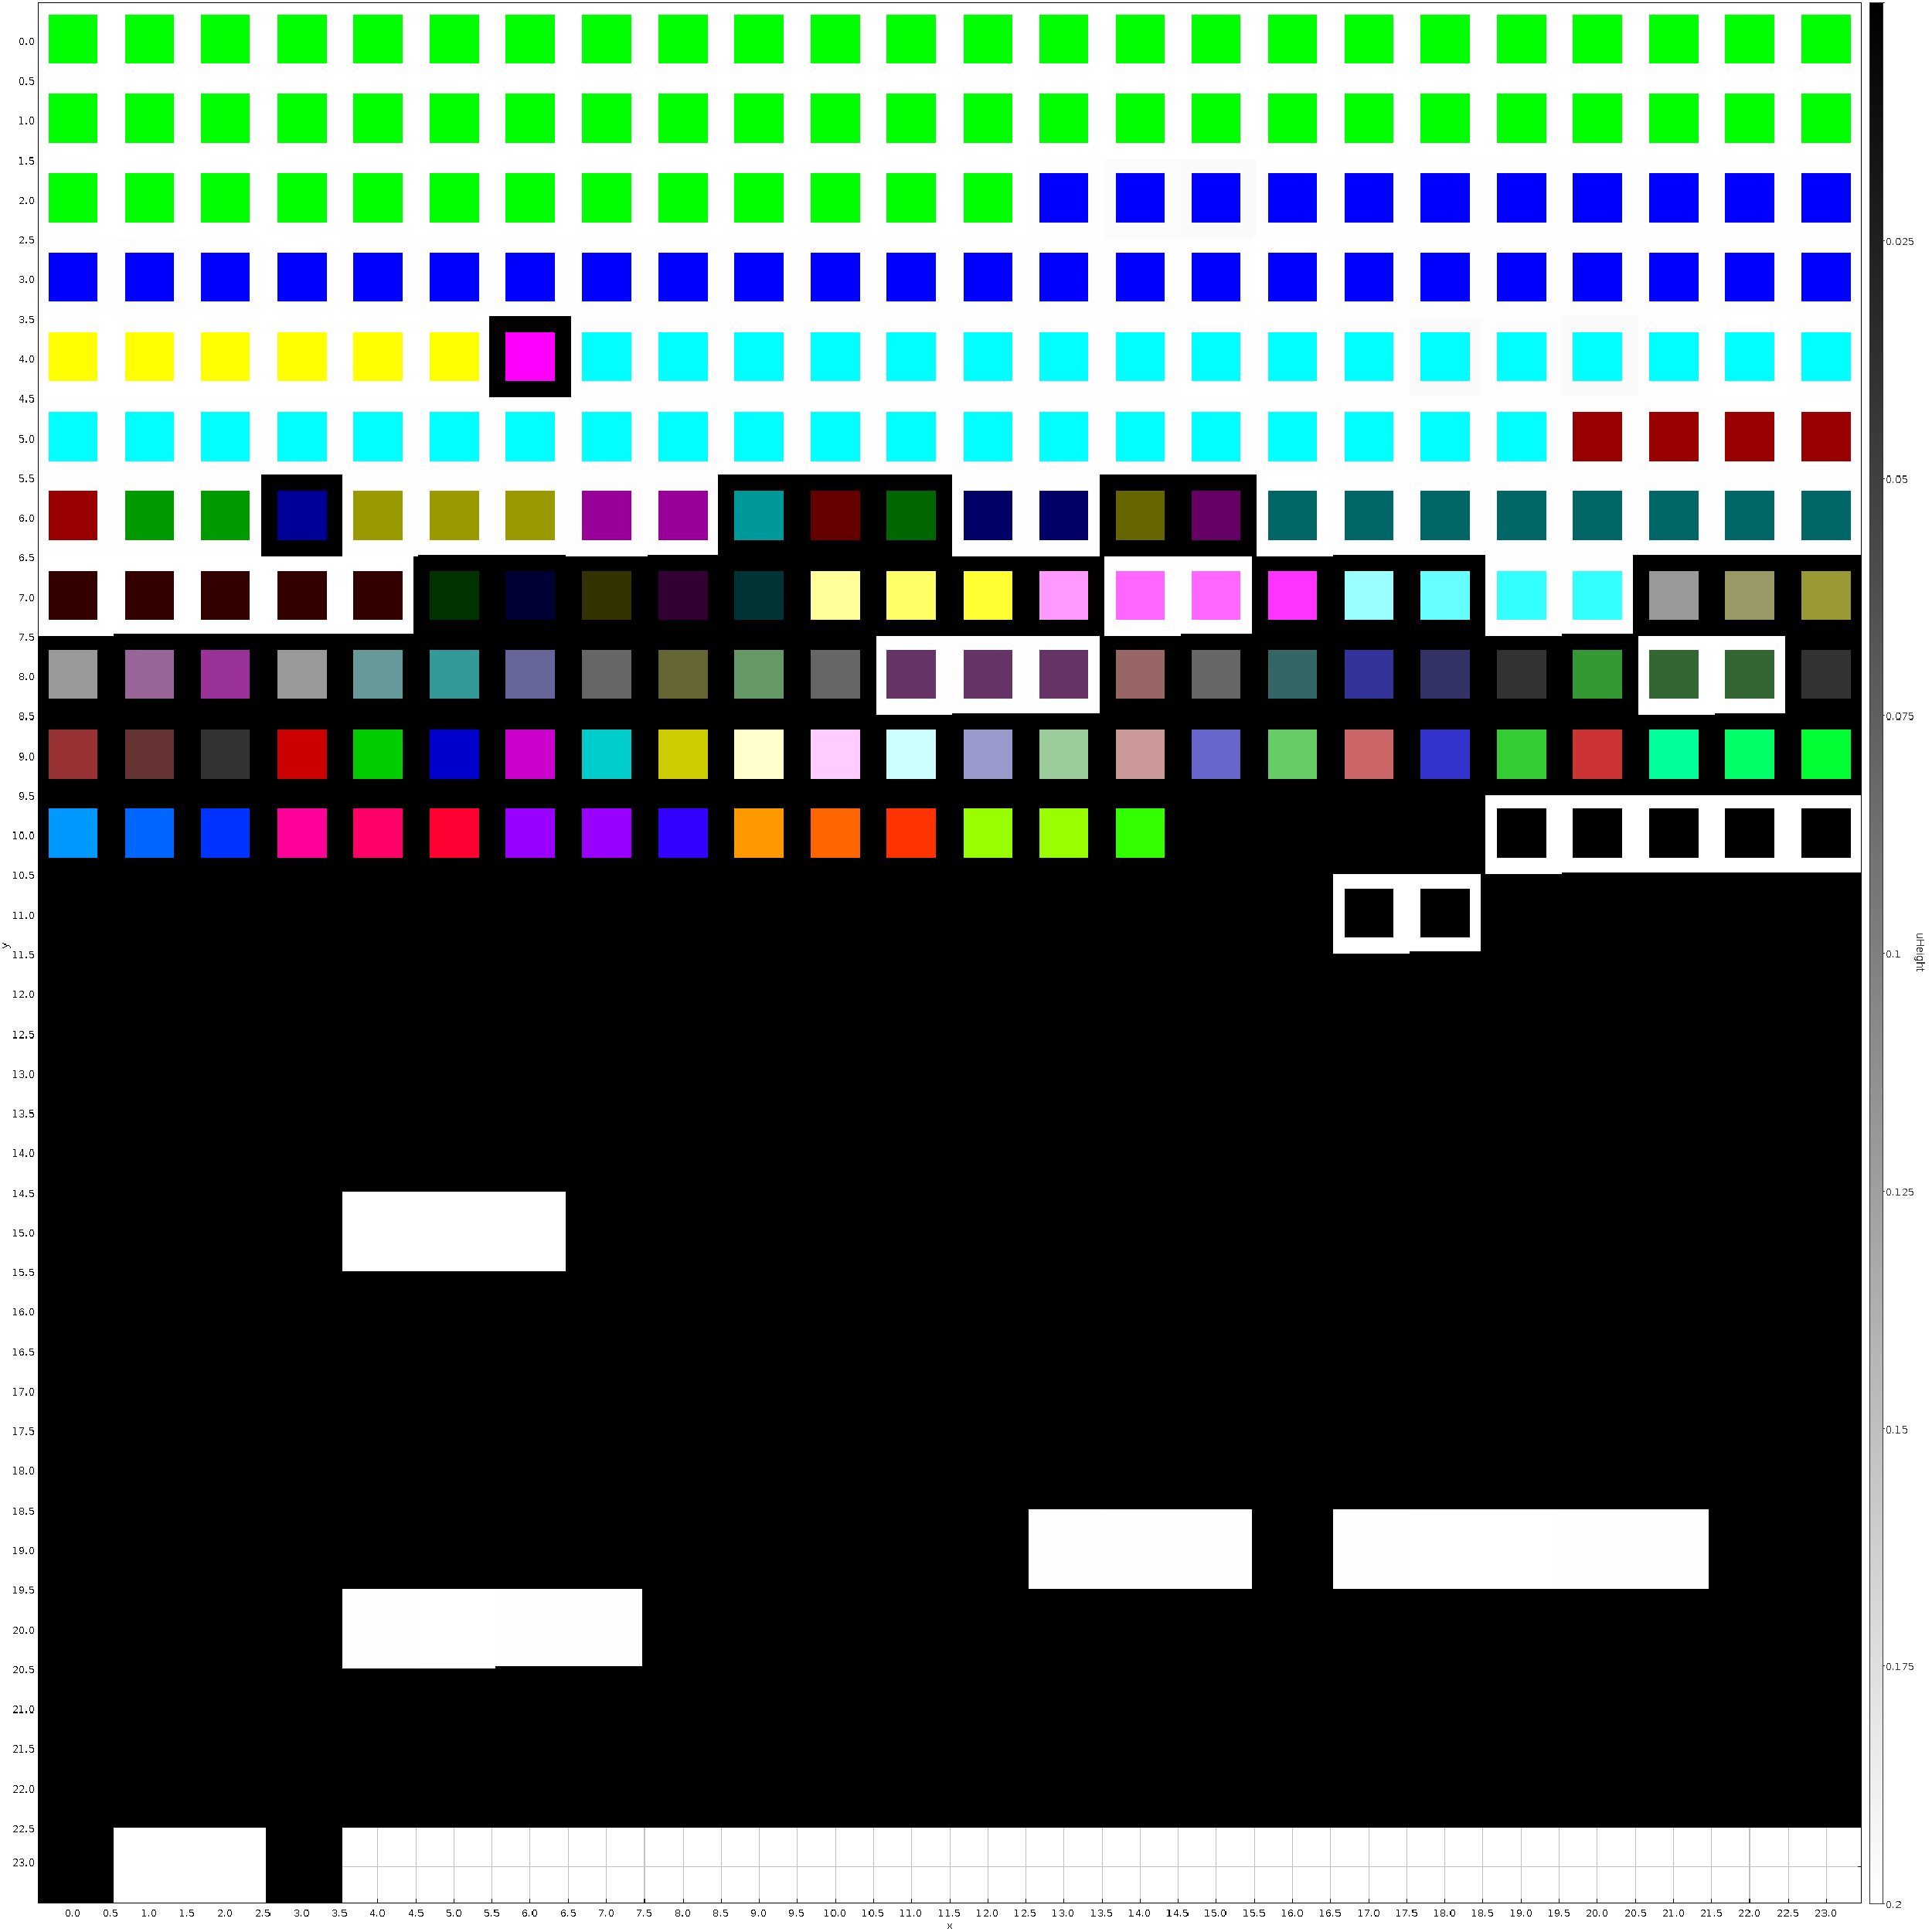
\includegraphics[width=0.31\textwidth]{matri6-01.png}
    \caption{All of the images correspond to U-matrices of the ended experiments mentioned above in order (Train2, Train3, Train6)}
    \label{img:matrixended}
\end{figure}
 There is work to be done for this cases, understand what is going on and interpret correctly the results, but last we got some.
\subsection{CSOM}
%one image
Well, as I mentioned before I did some tests using the ESOM method but since I wasn{t getting any results I thougth of testing this methond, as always I strongly recommend to read carefully its manual, \url{http://dame.dsf.unina.it/documents/SOFM_UserManual_DAME-MAN-NA-0014-Rel1.1.pdf} and fully undesrtand what is going on behind the curtains. In the meanwhile, this is my own explanation. This method uses FITS files, does not support datacubes, speciffically uses a neighborhood function in order to preserve the topological properties of the input space, it is a type of artificial network and is mainly unsupervised learning  and produces a low dimensional discretized representation of the input space of the training samples. I in this case you can choose the number of clusters/neurons in the first layer (neural network), the diameter, number of layers (in the neural network), learning rate and variance  on each layer. Here you have more input parameters to control.
\subsubsection{Expected Results}
Well in this case, since only FITS images are allowed, what we expect to find are areas indeitfying the different objects in the interstellar medium.

The important results in this case, are got in the \emph{Run} and \emph{Test} steps, in the \emph{Train} step only the network configuration is outputted. What we are interested on seein are the plotted clusters.
\subsubsection{Tests}
In this case I did some tests on the CSOM workspace, but none of the, where succesful, too many input variables to control and test. So, in this case I will leave this parameters free for you to try. I do believe that tis method could be very useful and if you find a way to input the datacube in a different configuration you will get some interesting results, due to the fact that in this method the preservation of the topology is one of the main principles.
%Mencionar los dos metodos de DAMEWARE
%Explicar los dos metodos, como untroduciste los datos, el objectivo de cada uno

%Lo que se espera obtener de cada uno de los experimentos, uno es en una sola imagen y el otro es en el datacube
%Los archivos que se obtienen y lo que significas, lo que se puede hacer



%Poner los parametros que se han elegido en los experimentos fallidos, y los que siguen en modo running
%Exlpicar por fases los experimentos que se intentaron


\section{Further work}
Well, finally we reached the point where I my time in Canada finished and I this research is still on its first stages. I have so many ideas of how to explore the clustering techniques in the DAME platform, MatLab, Python and everything else that can be tested. 

\subsection{Some interesting ideas}
%Normalizar los datos
%Acomodarlos y hacer que los paquetes sean mas pequeños
%Random points
For now, I would say that your best chance here, is to device an efficient way to input the information contained in a datacube as a list of points with values and reduce its dimensionality by randomly choosing them on every layer. If you are ever stuck, or no new ideas come to your mind, do not hesitate to contact me I might have a new interesting idea you can test.

\subsection{Links you should check out}
Most of them are listed in the useful resourses section of The Caltech-JPL Summer School on Big Data Analytics, the webpage \url{https://class.coursera.org/bigdataschool-001/wiki/Useful_resources}, you may need to create an account in Coursera and enroll in the course. And the rest of them are located in the References section on my GitHub page, \url{https://github.com/LaurethTeX/Clustering/blob/master/References.md}.
%Los links que estan en la pagina de el curso de caltech
%Sky surveys
%MATLAB SOM toolbox
%SAO datamining
\vfill
\textit{Wish you all the best, Andrea Hidalgo}

\end{document}